This documentation has been automatically generated from the simulator \texttt{UNISIM ppcemu-system} version 1.0beta5 on Oct 17 2013.
\subsection{Introduction}
UNISIM ppcemu-system is a full system simulator of a board including a MPC7447A PowerPC processor, a MPC107 chipset, and supporting Linux boot. The simulated board is very similar to a PowerMac G4 PCI machine. Computations on IEEE 754 floating point numbers are emulated using Simfloat++. Altivec instructions are currently decoded but not implemented. The running PowerPC application is a PowerMac Linux Kernel and all the applications installed on the hard disk image and/or the initial RAM disk image. Software running on the simulated hardware can be debugged by connecting a GDB client to the simulator through the GDB serial remote protocol. The GDB client can be either the standard text based client (i.e. command gdb), a graphical front-end to GDB (e.g. ddd), or even Eclipse CDT..\\
Section \ref{UNISIM ppcemu-system_licensing} gives licensing informations about the simulator.
Section \ref{UNISIM ppcemu-system_simulated_configuration} shows the set of modules and services that compose the simulator.
Section \ref{UNISIM ppcemu-system_using} shows how to invoke the simulator at the command line prompt.
Section \ref{UNISIM ppcemu-system_configuration} gives the simulator parameters.
Section \ref{UNISIM ppcemu-system_statistics} gives the simulator statistic counters.
Section \ref{UNISIM ppcemu-system_formulas} gives the simulator statistic formulas.
\subsection{Licensing}
\label{UNISIM ppcemu-system_licensing}
UNISIM ppcemu-system 1.0beta5\\
Copyright (C) 2007-2010, Commissariat a l'Energie Atomique (CEA)\\
License: BSD (see file COPYING)\\
Authors: Gilles Mouchard $<$gilles.mouchard@cea.fr$>$, Daniel Gracia P\'erez $<$daniel.gracia-perez@cea.fr$>$\\
\subsection{Simulated configuration}
\label{UNISIM ppcemu-system_simulated_configuration}
\begin{figure}[!ht]
	\begin{center}
		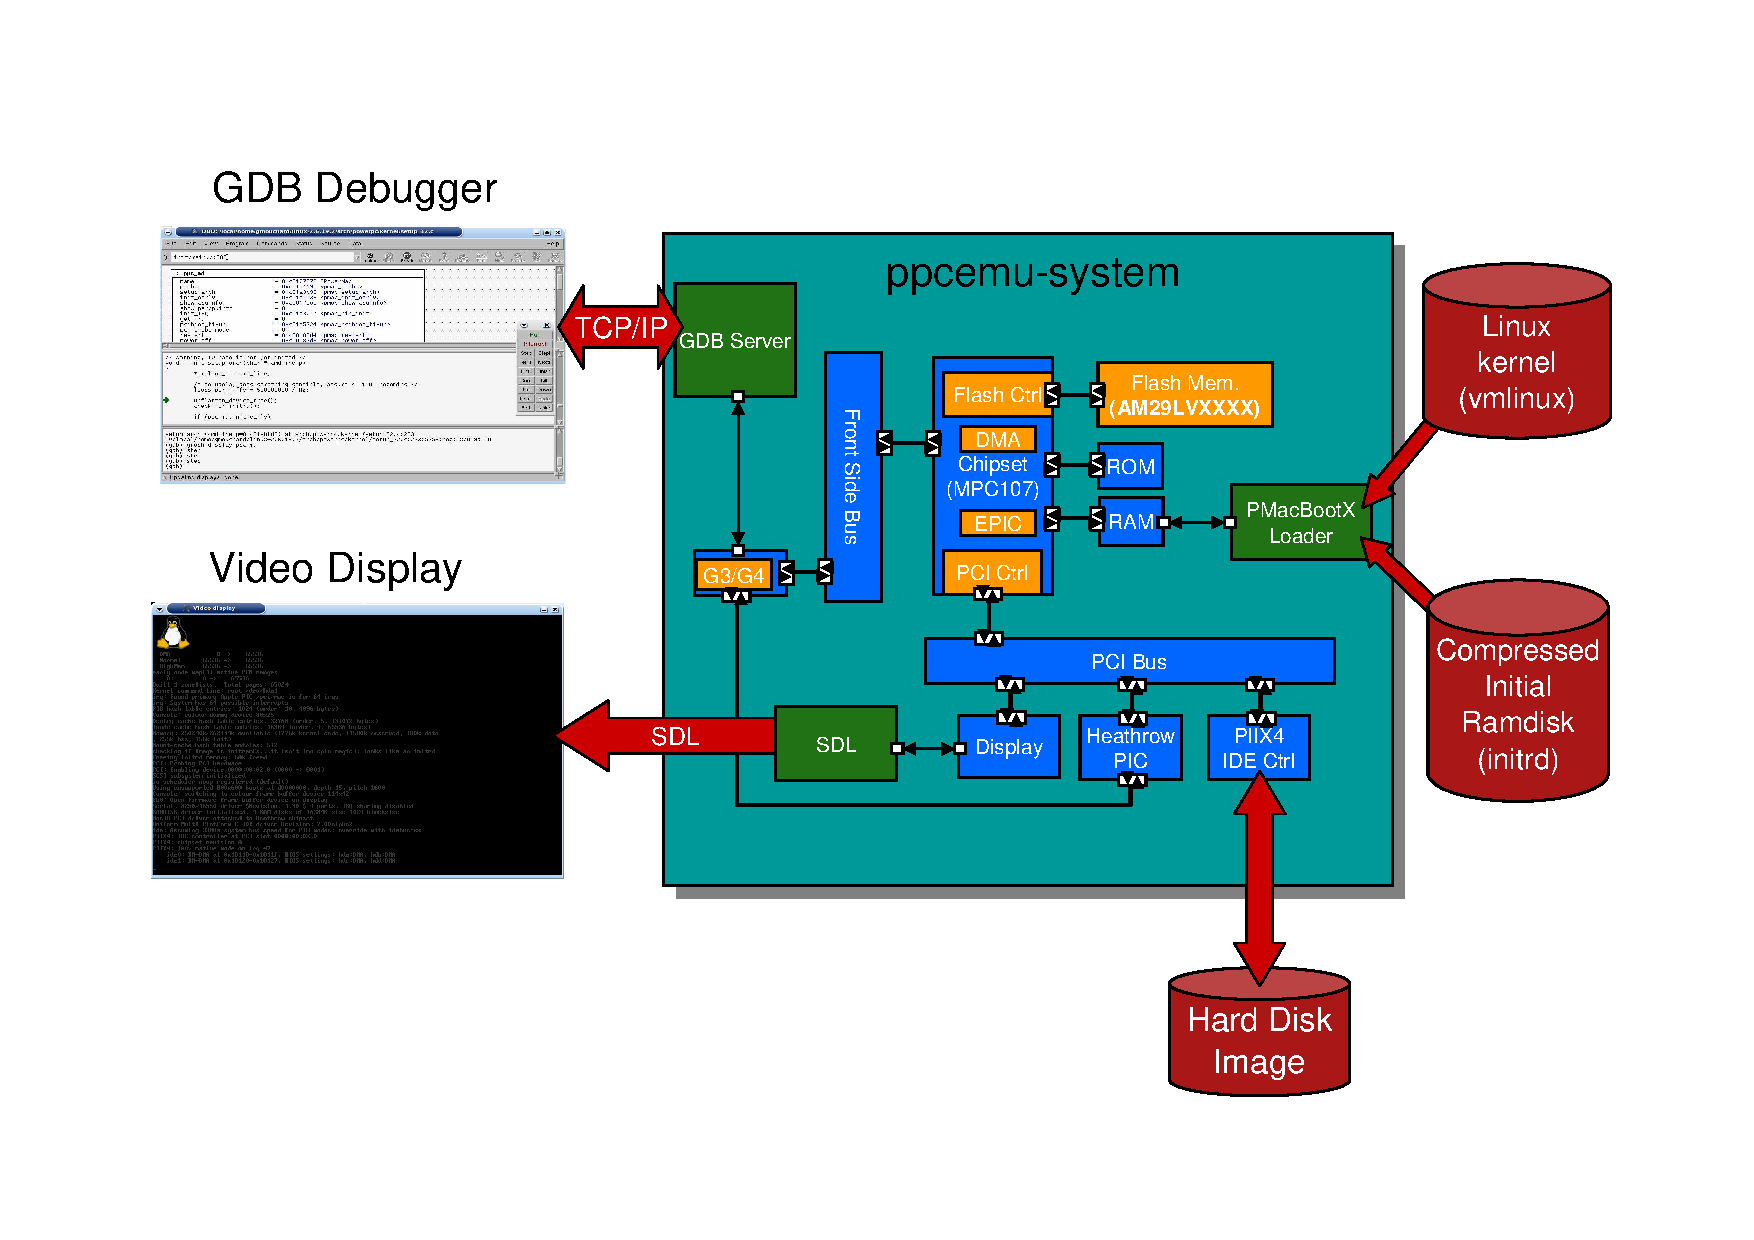
\includegraphics[width=\textwidth]{ppcemu_system/fig_schematic.pdf}
	\end{center}
	\caption{UNISIM ppcemu-system simulator schematic.}
\end{figure}
\noindent The UNISIM ppcemu-system simulator is composed of the following modules and services:
\begin{itemize}\addtolength{\itemsep}{-0.40\baselineskip}
\item \textbf{bus}: Front side bus
\item \textbf{cpu}: PowerPC MPC7447A CPU
\item \textbf{debugger}
\item \textbf{erom}: Memory
\item \textbf{flash}: This module implements an AM29LV800BT flash memory with the following characteristics:\\
Manufacturer ID: 0x010000\\
Device ID word \#0: 0xda2202\\
Size: 4194304 bytes\\
I/O width: 64 bits\\
Number of chips: 4 chips\\
I/O width per chip: 16 bits\\
Size per chip: 1048576 bytes\\
Number of Sectors: 19 sectors\\
8-bit mode support: yes\\
16-bit mode support: yes\\
Access time: 70 ns\\
Byte programming time: 9000 us\\
Word programming time: 110000 us\\
Sector erasing time: 700000000 us\\
Chip erasing time: 14000000000 us\\

\item \textbf{gdb-server}: this service implements the GDB server remote serial protocol over TCP/IP. Standards GDB clients (e.g. gdb, eclipse, ddd) can connect to the simulator to debug the target application that runs within the simulator.
\item \textbf{heathrow}: Heathrow Programmable Interrupt Controller (PIC)
\item \textbf{host-time}: this service is an abstraction layer for the host machine time
\item \textbf{i8042}: i8042 PS/2 keyboard/mouse controller
\item \textbf{inline-debugger}: this service implements a built-in debugger in the terminal console
\item \textbf{memory}: Memory
\item \textbf{mpc107}: MPC107 chipset
\item \textbf{mpc107.DMA}: MPC107 integrated Direct Memory Access (DMA) controller
\item \textbf{mpc107.address\_mapper}: MPC107 Address mapper
\item \textbf{mpc107.atu}: MPC107 integrated Address Translation Unit (ATU)
\item \textbf{mpc107.epic}: MPC107 integrated Embedded Programmable Interrupt Controller (EPIC)
\item \textbf{mpc107.pci\_controller}: MPC107 integrated PCI bus controller
\item \textbf{pci-bus}: PCI bus
\item \textbf{pci-display}: PCI Video frame buffer display
\item \textbf{pci-ide}: PIIX4 IDE controller
\item \textbf{pci-isa-bridge}: PCI-to-ISA bridge
\item \textbf{pmac-linux-kernel-loader}: PowerMac Linux kernel loader
\item \textbf{pmac-linux-kernel-loader.elf32-loader}: this service implements an ELF32 Loader
\item \textbf{pmac-linux-kernel-loader.pmac-bootx}: This service is a PowerMac BootX loader emulator. It allows bootloading a PowerMac Linux kernel with its initial ramdisk and device tree
\item \textbf{profiler}
\item \textbf{sdl}: SDL (Simple DirectMedia Layer) wrapper
\item \textbf{tee-memory-access-reporting}
\item \textbf{tee-memory-access-reporting.tee-memory-access-reporting.control\_selector[0]}
\item \textbf{tee-memory-access-reporting.tee-memory-access-reporting.control\_selector[10]}
\item \textbf{tee-memory-access-reporting.tee-memory-access-reporting.control\_selector[11]}
\item \textbf{tee-memory-access-reporting.tee-memory-access-reporting.control\_selector[12]}
\item \textbf{tee-memory-access-reporting.tee-memory-access-reporting.control\_selector[13]}
\item \textbf{tee-memory-access-reporting.tee-memory-access-reporting.control\_selector[14]}
\item \textbf{tee-memory-access-reporting.tee-memory-access-reporting.control\_selector[15]}
\item \textbf{tee-memory-access-reporting.tee-memory-access-reporting.control\_selector[1]}
\item \textbf{tee-memory-access-reporting.tee-memory-access-reporting.control\_selector[2]}
\item \textbf{tee-memory-access-reporting.tee-memory-access-reporting.control\_selector[3]}
\item \textbf{tee-memory-access-reporting.tee-memory-access-reporting.control\_selector[4]}
\item \textbf{tee-memory-access-reporting.tee-memory-access-reporting.control\_selector[5]}
\item \textbf{tee-memory-access-reporting.tee-memory-access-reporting.control\_selector[6]}
\item \textbf{tee-memory-access-reporting.tee-memory-access-reporting.control\_selector[7]}
\item \textbf{tee-memory-access-reporting.tee-memory-access-reporting.control\_selector[8]}
\item \textbf{tee-memory-access-reporting.tee-memory-access-reporting.control\_selector[9]}
\item \textbf{time}: this service is an abstraction layer for the SystemC kernel time
\end{itemize}
\subsection{Using the UNISIM ppcemu-system simulator}
\label{UNISIM ppcemu-system_using}
The UNISIM ppcemu-system simulator has the following command line options:\\
~\\
\noindent Usage: \texttt{unisim-ppcemu-system-1.0beta5 [<options>] [...]}

\noindent Options:
\begin{itemize}
\item \texttt{--set $<$param=value$>$ or -s $<$param=value$>$}: set value of parameter 'param' to 'value'
\item \texttt{--config $<$XML file$>$ or -c $<$XML file$>$}: configures the simulator with the given XML configuration file
\item \texttt{--get-config $<$XML file$>$ or -g $<$XML file$>$}: get the simulator configuration XML file (you can use it to create your own configuration. This option can be combined with -c to get a new configuration file with existing variables from another file
\item \texttt{--list or -l}: lists all available parameters, their type, and their current value
\item \texttt{--warn or -w}: enable printing of kernel warnings
\item \texttt{--doc $<$Latex file$>$ or -d $<$Latex file$>$}: enable printing a latex documentation
\item \texttt{--version or -v}: displays the program version information
\item \texttt{--share-path $<$path$>$ or -p $<$path$>$}: the path that should be used for the share directory (absolute path)
\item \texttt{--help or -h}: displays this help
\end{itemize}
\subsection{Configuration}
\label{UNISIM ppcemu-system_configuration}
Simulator configuration (see below) can be modified using command line Options \texttt{--set $<$param=value$>$} or \texttt{--config $<$config file$>$}.\\
~\\
\tablehead{\hline}
\tabletail{\hline}
\begin{supertabular}{|p{7.5cm}|p{7.5cm}|}
\multicolumn{2}{|l|}{\textbf{\Large Global}}\\
\hline
\multicolumn{1}{|p{7.5cm}}{\textbf{Name:} \texttt{enable-gdb-server}} & \multicolumn{1}{p{7.5cm}|}{\textbf{Type:} \texttt{parameter}}\\
\multicolumn{1}{|p{7.5cm}}{\textbf{Default:} \texttt{true}} & \multicolumn{1}{p{7.5cm}|}{\textbf{Data type:} \texttt{boolean}}\\
\multicolumn{2}{|p{15cm}|}{\textbf{Valid:} \texttt{true},~\texttt{false}}\\
\multicolumn{2}{|l|}{}\\
\multicolumn{2}{|p{15cm}|}{\textbf{Description:} \newline Enable/Disable GDB server instantiation.}\\
\hline
\multicolumn{1}{|p{7.5cm}}{\textbf{Name:} \texttt{enable-inline-debugger}} & \multicolumn{1}{p{7.5cm}|}{\textbf{Type:} \texttt{parameter}}\\
\multicolumn{1}{|p{7.5cm}}{\textbf{Default:} \texttt{true}} & \multicolumn{1}{p{7.5cm}|}{\textbf{Data type:} \texttt{boolean}}\\
\multicolumn{2}{|p{15cm}|}{\textbf{Valid:} \texttt{true},~\texttt{false}}\\
\multicolumn{2}{|l|}{}\\
\multicolumn{2}{|p{15cm}|}{\textbf{Description:} \newline Enable/Disable inline debugger instantiation.}\\
\hline
\multicolumn{1}{|p{7.5cm}}{\textbf{Name:} \texttt{enable-press-enter-at-exit}} & \multicolumn{1}{p{7.5cm}|}{\textbf{Type:} \texttt{parameter}}\\
\multicolumn{1}{|p{7.5cm}}{\textbf{Default:} \texttt{false}} & \multicolumn{1}{p{7.5cm}|}{\textbf{Data type:} \texttt{boolean}}\\
\multicolumn{2}{|p{15cm}|}{\textbf{Valid:} \texttt{true},~\texttt{false}}\\
\multicolumn{2}{|l|}{}\\
\multicolumn{2}{|p{15cm}|}{\textbf{Description:} \newline Enable/Disable pressing key enter at exit.}\\
\hline
\multicolumn{1}{|p{7.5cm}}{\textbf{Name:} \texttt{estimate-power}} & \multicolumn{1}{p{7.5cm}|}{\textbf{Type:} \texttt{parameter}}\\
\multicolumn{1}{|p{7.5cm}}{\textbf{Default:} \texttt{false}} & \multicolumn{1}{p{7.5cm}|}{\textbf{Data type:} \texttt{boolean}}\\
\multicolumn{2}{|p{15cm}|}{\textbf{Valid:} \texttt{true},~\texttt{false}}\\
\multicolumn{2}{|l|}{}\\
\multicolumn{2}{|p{15cm}|}{\textbf{Description:} \newline Enable/Disable power estimators instantiation.}\\
\hline
\multicolumn{1}{|p{7.5cm}}{\textbf{Name:} \texttt{kernel\_logger.file}} & \multicolumn{1}{p{7.5cm}|}{\textbf{Type:} \texttt{parameter}}\\
\multicolumn{1}{|p{7.5cm}}{\textbf{Default:} \texttt{false}} & \multicolumn{1}{p{7.5cm}|}{\textbf{Data type:} \texttt{boolean}}\\
\multicolumn{2}{|p{15cm}|}{\textbf{Valid:} \texttt{true},~\texttt{false}}\\
\multicolumn{2}{|l|}{}\\
\multicolumn{2}{|p{15cm}|}{\textbf{Description:} \newline Keep logger output in a file.}\\
\hline
\multicolumn{1}{|p{7.5cm}}{\textbf{Name:} \texttt{kernel\_logger.filename}} & \multicolumn{1}{p{7.5cm}|}{\textbf{Type:} \texttt{parameter}}\\
\multicolumn{1}{|p{7.5cm}}{\textbf{Default:} \texttt{logger\_output.txt}} & \multicolumn{1}{p{7.5cm}|}{\textbf{Data type:} \texttt{string}}\\
\multicolumn{2}{|l|}{}\\
\multicolumn{2}{|l|}{}\\
\multicolumn{2}{|p{15cm}|}{\textbf{Description:} \newline Filename to keep logger output \_(the option file must be activated).}\\
\hline
\multicolumn{1}{|p{7.5cm}}{\textbf{Name:} \texttt{kernel\_logger.std\_err}} & \multicolumn{1}{p{7.5cm}|}{\textbf{Type:} \texttt{parameter}}\\
\multicolumn{1}{|p{7.5cm}}{\textbf{Default:} \texttt{true}} & \multicolumn{1}{p{7.5cm}|}{\textbf{Data type:} \texttt{boolean}}\\
\multicolumn{2}{|p{15cm}|}{\textbf{Valid:} \texttt{true},~\texttt{false}}\\
\multicolumn{2}{|l|}{}\\
\multicolumn{2}{|p{15cm}|}{\textbf{Description:} \newline Show logger output through the standard error output.}\\
\hline
\multicolumn{1}{|p{7.5cm}}{\textbf{Name:} \texttt{kernel\_logger.std\_err\_color}} & \multicolumn{1}{p{7.5cm}|}{\textbf{Type:} \texttt{parameter}}\\
\multicolumn{1}{|p{7.5cm}}{\textbf{Default:} \texttt{false}} & \multicolumn{1}{p{7.5cm}|}{\textbf{Data type:} \texttt{boolean}}\\
\multicolumn{2}{|p{15cm}|}{\textbf{Valid:} \texttt{true},~\texttt{false}}\\
\multicolumn{2}{|l|}{}\\
\multicolumn{2}{|p{15cm}|}{\textbf{Description:} \newline Colorize logger output through the standard error output \_(only works if std\_err is active).}\\
\hline
\multicolumn{1}{|p{7.5cm}}{\textbf{Name:} \texttt{kernel\_logger.std\_out}} & \multicolumn{1}{p{7.5cm}|}{\textbf{Type:} \texttt{parameter}}\\
\multicolumn{1}{|p{7.5cm}}{\textbf{Default:} \texttt{false}} & \multicolumn{1}{p{7.5cm}|}{\textbf{Data type:} \texttt{boolean}}\\
\multicolumn{2}{|p{15cm}|}{\textbf{Valid:} \texttt{true},~\texttt{false}}\\
\multicolumn{2}{|l|}{}\\
\multicolumn{2}{|p{15cm}|}{\textbf{Description:} \newline Show logger output through the standard output.}\\
\hline
\multicolumn{1}{|p{7.5cm}}{\textbf{Name:} \texttt{kernel\_logger.std\_out\_color}} & \multicolumn{1}{p{7.5cm}|}{\textbf{Type:} \texttt{parameter}}\\
\multicolumn{1}{|p{7.5cm}}{\textbf{Default:} \texttt{false}} & \multicolumn{1}{p{7.5cm}|}{\textbf{Data type:} \texttt{boolean}}\\
\multicolumn{2}{|p{15cm}|}{\textbf{Valid:} \texttt{true},~\texttt{false}}\\
\multicolumn{2}{|l|}{}\\
\multicolumn{2}{|p{15cm}|}{\textbf{Description:} \newline Colorize logger output through the standard output \_(only works if std\_out is active).}\\
\hline
\multicolumn{1}{|p{7.5cm}}{\textbf{Name:} \texttt{kernel\_logger.xml\_file}} & \multicolumn{1}{p{7.5cm}|}{\textbf{Type:} \texttt{parameter}}\\
\multicolumn{1}{|p{7.5cm}}{\textbf{Default:} \texttt{false}} & \multicolumn{1}{p{7.5cm}|}{\textbf{Data type:} \texttt{boolean}}\\
\multicolumn{2}{|p{15cm}|}{\textbf{Valid:} \texttt{true},~\texttt{false}}\\
\multicolumn{2}{|l|}{}\\
\multicolumn{2}{|p{15cm}|}{\textbf{Description:} \newline Keep logger output in a file xml formatted.}\\
\hline
\multicolumn{1}{|p{7.5cm}}{\textbf{Name:} \texttt{kernel\_logger.xml\_file\_gzipped}} & \multicolumn{1}{p{7.5cm}|}{\textbf{Type:} \texttt{parameter}}\\
\multicolumn{1}{|p{7.5cm}}{\textbf{Default:} \texttt{false}} & \multicolumn{1}{p{7.5cm}|}{\textbf{Data type:} \texttt{boolean}}\\
\multicolumn{2}{|p{15cm}|}{\textbf{Valid:} \texttt{true},~\texttt{false}}\\
\multicolumn{2}{|l|}{}\\
\multicolumn{2}{|p{15cm}|}{\textbf{Description:} \newline If the xml\_file option is active, the output file will be compressed (a .gz extension will be automatically added to the xml\_filename option.}\\
\hline
\multicolumn{1}{|p{7.5cm}}{\textbf{Name:} \texttt{kernel\_logger.xml\_filename}} & \multicolumn{1}{p{7.5cm}|}{\textbf{Type:} \texttt{parameter}}\\
\multicolumn{1}{|p{7.5cm}}{\textbf{Default:} \texttt{logger\_output.xml}} & \multicolumn{1}{p{7.5cm}|}{\textbf{Data type:} \texttt{string}}\\
\multicolumn{2}{|l|}{}\\
\multicolumn{2}{|l|}{}\\
\multicolumn{2}{|p{15cm}|}{\textbf{Description:} \newline Filename to keep logger xml output \_(the option xml\_file must be activated).}\\
\hline
\multicolumn{1}{|p{7.5cm}}{\textbf{Name:} \texttt{message-spy}} & \multicolumn{1}{p{7.5cm}|}{\textbf{Type:} \texttt{parameter}}\\
\multicolumn{1}{|p{7.5cm}}{\textbf{Default:} \texttt{false}} & \multicolumn{1}{p{7.5cm}|}{\textbf{Data type:} \texttt{boolean}}\\
\multicolumn{2}{|p{15cm}|}{\textbf{Valid:} \texttt{true},~\texttt{false}}\\
\multicolumn{2}{|l|}{}\\
\multicolumn{2}{|p{15cm}|}{\textbf{Description:} \newline Enable/Disable message spies instantiation.}\\
\hline
\hline
\multicolumn{2}{|l|}{\textbf{\Large bus}}\\
\hline
\multicolumn{1}{|p{7.5cm}}{\textbf{Name:} \texttt{bus.verbose}} & \multicolumn{1}{p{7.5cm}|}{\textbf{Type:} \texttt{parameter}}\\
\multicolumn{1}{|p{7.5cm}}{\textbf{Default:} \texttt{false}} & \multicolumn{1}{p{7.5cm}|}{\textbf{Data type:} \texttt{boolean}}\\
\multicolumn{2}{|p{15cm}|}{\textbf{Valid:} \texttt{true},~\texttt{false}}\\
\multicolumn{2}{|l|}{}\\
\multicolumn{2}{|p{15cm}|}{\textbf{Description:} \newline enable/disable verbosity.}\\
\hline
\multicolumn{1}{|p{7.5cm}}{\textbf{Name:} \texttt{bus.cycle-time}} & \multicolumn{1}{p{7.5cm}|}{\textbf{Type:} \texttt{parameter}}\\
\multicolumn{1}{|p{7.5cm}}{\textbf{Default:} \texttt{13333 ps}} & \multicolumn{1}{p{7.5cm}|}{\textbf{Data type:} \texttt{sc\_time}}\\
\multicolumn{2}{|l|}{}\\
\multicolumn{2}{|l|}{}\\
\multicolumn{2}{|p{15cm}|}{\textbf{Description:} \newline cycle time.}\\
\hline
\hline
\multicolumn{2}{|l|}{\textbf{\Large cpu}}\\
\hline
\multicolumn{1}{|p{7.5cm}}{\textbf{Name:} \texttt{cpu.cpu-cycle-time}} & \multicolumn{1}{p{7.5cm}|}{\textbf{Type:} \texttt{parameter}}\\
\multicolumn{1}{|p{7.5cm}}{\textbf{Default:} \texttt{3333}} & \multicolumn{1}{p{7.5cm}|}{\textbf{Data type:} \texttt{unsigned 64-bit integer}}\\
\multicolumn{2}{|l|}{}\\
\multicolumn{2}{|l|}{}\\
\multicolumn{2}{|p{15cm}|}{\textbf{Description:} \newline CPU cycle time in picoseconds.}\\
\hline
\multicolumn{1}{|p{7.5cm}}{\textbf{Name:} \texttt{cpu.voltage}} & \multicolumn{1}{p{7.5cm}|}{\textbf{Type:} \texttt{parameter}}\\
\multicolumn{1}{|p{7.5cm}}{\textbf{Default:} \texttt{1300}} & \multicolumn{1}{p{7.5cm}|}{\textbf{Data type:} \texttt{unsigned 64-bit integer}}\\
\multicolumn{2}{|l|}{}\\
\multicolumn{2}{|l|}{}\\
\multicolumn{2}{|p{15cm}|}{\textbf{Description:} \newline CPU voltage in mV.}\\
\hline
\multicolumn{1}{|p{7.5cm}}{\textbf{Name:} \texttt{cpu.max-inst}} & \multicolumn{1}{p{7.5cm}|}{\textbf{Type:} \texttt{parameter}}\\
\multicolumn{1}{|p{7.5cm}}{\textbf{Default:} \texttt{18446744073709551615}} & \multicolumn{1}{p{7.5cm}|}{\textbf{Data type:} \texttt{unsigned 64-bit integer}}\\
\multicolumn{2}{|l|}{}\\
\multicolumn{2}{|l|}{}\\
\multicolumn{2}{|p{15cm}|}{\textbf{Description:} \newline maximum number of instructions to simulate.}\\
\hline
\multicolumn{1}{|p{7.5cm}}{\textbf{Name:} \texttt{cpu.verbose-all}} & \multicolumn{1}{p{7.5cm}|}{\textbf{Type:} \texttt{parameter}}\\
\multicolumn{1}{|p{7.5cm}}{\textbf{Default:} \texttt{false}} & \multicolumn{1}{p{7.5cm}|}{\textbf{Data type:} \texttt{boolean}}\\
\multicolumn{2}{|p{15cm}|}{\textbf{Valid:} \texttt{true},~\texttt{false}}\\
\multicolumn{2}{|l|}{}\\
\multicolumn{2}{|p{15cm}|}{\textbf{Description:} \newline globally enable/disable verbosity.}\\
\hline
\multicolumn{1}{|p{7.5cm}}{\textbf{Name:} \texttt{cpu.verbose-setup}} & \multicolumn{1}{p{7.5cm}|}{\textbf{Type:} \texttt{parameter}}\\
\multicolumn{1}{|p{7.5cm}}{\textbf{Default:} \texttt{false}} & \multicolumn{1}{p{7.5cm}|}{\textbf{Data type:} \texttt{boolean}}\\
\multicolumn{2}{|p{15cm}|}{\textbf{Valid:} \texttt{true},~\texttt{false}}\\
\multicolumn{2}{|l|}{}\\
\multicolumn{2}{|p{15cm}|}{\textbf{Description:} \newline enable/disable verbosity while setup.}\\
\hline
\multicolumn{1}{|p{7.5cm}}{\textbf{Name:} \texttt{cpu.verbose-step}} & \multicolumn{1}{p{7.5cm}|}{\textbf{Type:} \texttt{parameter}}\\
\multicolumn{1}{|p{7.5cm}}{\textbf{Default:} \texttt{false}} & \multicolumn{1}{p{7.5cm}|}{\textbf{Data type:} \texttt{boolean}}\\
\multicolumn{2}{|p{15cm}|}{\textbf{Valid:} \texttt{true},~\texttt{false}}\\
\multicolumn{2}{|l|}{}\\
\multicolumn{2}{|p{15cm}|}{\textbf{Description:} \newline enable/disable verbosity when simulating an instruction.}\\
\hline
\multicolumn{1}{|p{7.5cm}}{\textbf{Name:} \texttt{cpu.verbose-dtlb}} & \multicolumn{1}{p{7.5cm}|}{\textbf{Type:} \texttt{parameter}}\\
\multicolumn{1}{|p{7.5cm}}{\textbf{Default:} \texttt{false}} & \multicolumn{1}{p{7.5cm}|}{\textbf{Data type:} \texttt{boolean}}\\
\multicolumn{2}{|p{15cm}|}{\textbf{Valid:} \texttt{true},~\texttt{false}}\\
\multicolumn{2}{|l|}{}\\
\multicolumn{2}{|p{15cm}|}{\textbf{Description:} \newline enable/disable verbosity when accessing data translation lookahead buffer.}\\
\hline
\multicolumn{1}{|p{7.5cm}}{\textbf{Name:} \texttt{cpu.verbose-itlb}} & \multicolumn{1}{p{7.5cm}|}{\textbf{Type:} \texttt{parameter}}\\
\multicolumn{1}{|p{7.5cm}}{\textbf{Default:} \texttt{false}} & \multicolumn{1}{p{7.5cm}|}{\textbf{Data type:} \texttt{boolean}}\\
\multicolumn{2}{|p{15cm}|}{\textbf{Valid:} \texttt{true},~\texttt{false}}\\
\multicolumn{2}{|l|}{}\\
\multicolumn{2}{|p{15cm}|}{\textbf{Description:} \newline enable/disable verbosity when accessing instruction translation lookahead buffer.}\\
\hline
\multicolumn{1}{|p{7.5cm}}{\textbf{Name:} \texttt{cpu.verbose-dl1}} & \multicolumn{1}{p{7.5cm}|}{\textbf{Type:} \texttt{parameter}}\\
\multicolumn{1}{|p{7.5cm}}{\textbf{Default:} \texttt{false}} & \multicolumn{1}{p{7.5cm}|}{\textbf{Data type:} \texttt{boolean}}\\
\multicolumn{2}{|p{15cm}|}{\textbf{Valid:} \texttt{true},~\texttt{false}}\\
\multicolumn{2}{|l|}{}\\
\multicolumn{2}{|p{15cm}|}{\textbf{Description:} \newline enable/disable verbosity when accessing L1 data cache.}\\
\hline
\multicolumn{1}{|p{7.5cm}}{\textbf{Name:} \texttt{cpu.verbose-il1}} & \multicolumn{1}{p{7.5cm}|}{\textbf{Type:} \texttt{parameter}}\\
\multicolumn{1}{|p{7.5cm}}{\textbf{Default:} \texttt{false}} & \multicolumn{1}{p{7.5cm}|}{\textbf{Data type:} \texttt{boolean}}\\
\multicolumn{2}{|p{15cm}|}{\textbf{Valid:} \texttt{true},~\texttt{false}}\\
\multicolumn{2}{|l|}{}\\
\multicolumn{2}{|p{15cm}|}{\textbf{Description:} \newline enable/disable verbosity when accessing L1 instruction cache.}\\
\hline
\multicolumn{1}{|p{7.5cm}}{\textbf{Name:} \texttt{cpu.verbose-l2}} & \multicolumn{1}{p{7.5cm}|}{\textbf{Type:} \texttt{parameter}}\\
\multicolumn{1}{|p{7.5cm}}{\textbf{Default:} \texttt{false}} & \multicolumn{1}{p{7.5cm}|}{\textbf{Data type:} \texttt{boolean}}\\
\multicolumn{2}{|p{15cm}|}{\textbf{Valid:} \texttt{true},~\texttt{false}}\\
\multicolumn{2}{|l|}{}\\
\multicolumn{2}{|p{15cm}|}{\textbf{Description:} \newline enable/disable verbosity when accessing L2 unified cache.}\\
\hline
\multicolumn{1}{|p{7.5cm}}{\textbf{Name:} \texttt{cpu.verbose-load}} & \multicolumn{1}{p{7.5cm}|}{\textbf{Type:} \texttt{parameter}}\\
\multicolumn{1}{|p{7.5cm}}{\textbf{Default:} \texttt{false}} & \multicolumn{1}{p{7.5cm}|}{\textbf{Data type:} \texttt{boolean}}\\
\multicolumn{2}{|p{15cm}|}{\textbf{Valid:} \texttt{true},~\texttt{false}}\\
\multicolumn{2}{|l|}{}\\
\multicolumn{2}{|p{15cm}|}{\textbf{Description:} \newline enable/disable verbosity when simulating a load.}\\
\hline
\multicolumn{1}{|p{7.5cm}}{\textbf{Name:} \texttt{cpu.verbose-store}} & \multicolumn{1}{p{7.5cm}|}{\textbf{Type:} \texttt{parameter}}\\
\multicolumn{1}{|p{7.5cm}}{\textbf{Default:} \texttt{false}} & \multicolumn{1}{p{7.5cm}|}{\textbf{Data type:} \texttt{boolean}}\\
\multicolumn{2}{|p{15cm}|}{\textbf{Valid:} \texttt{true},~\texttt{false}}\\
\multicolumn{2}{|l|}{}\\
\multicolumn{2}{|p{15cm}|}{\textbf{Description:} \newline enable/disable verbosity when simulating a store.}\\
\hline
\multicolumn{1}{|p{7.5cm}}{\textbf{Name:} \texttt{cpu.verbose-read-memory}} & \multicolumn{1}{p{7.5cm}|}{\textbf{Type:} \texttt{parameter}}\\
\multicolumn{1}{|p{7.5cm}}{\textbf{Default:} \texttt{false}} & \multicolumn{1}{p{7.5cm}|}{\textbf{Data type:} \texttt{boolean}}\\
\multicolumn{2}{|p{15cm}|}{\textbf{Valid:} \texttt{true},~\texttt{false}}\\
\multicolumn{2}{|l|}{}\\
\multicolumn{2}{|p{15cm}|}{\textbf{Description:} \newline enable/disable verbosity when reading memory for a debug purpose.}\\
\hline
\multicolumn{1}{|p{7.5cm}}{\textbf{Name:} \texttt{cpu.verbose-write-memory}} & \multicolumn{1}{p{7.5cm}|}{\textbf{Type:} \texttt{parameter}}\\
\multicolumn{1}{|p{7.5cm}}{\textbf{Default:} \texttt{false}} & \multicolumn{1}{p{7.5cm}|}{\textbf{Data type:} \texttt{boolean}}\\
\multicolumn{2}{|p{15cm}|}{\textbf{Valid:} \texttt{true},~\texttt{false}}\\
\multicolumn{2}{|l|}{}\\
\multicolumn{2}{|p{15cm}|}{\textbf{Description:} \newline enable/disable verbosity when writing memory for a debug purpose.}\\
\hline
\multicolumn{1}{|p{7.5cm}}{\textbf{Name:} \texttt{cpu.verbose-exception}} & \multicolumn{1}{p{7.5cm}|}{\textbf{Type:} \texttt{parameter}}\\
\multicolumn{1}{|p{7.5cm}}{\textbf{Default:} \texttt{false}} & \multicolumn{1}{p{7.5cm}|}{\textbf{Data type:} \texttt{boolean}}\\
\multicolumn{2}{|p{15cm}|}{\textbf{Valid:} \texttt{true},~\texttt{false}}\\
\multicolumn{2}{|l|}{}\\
\multicolumn{2}{|p{15cm}|}{\textbf{Description:} \newline enable/disable verbosity when handling exceptions.}\\
\hline
\multicolumn{1}{|p{7.5cm}}{\textbf{Name:} \texttt{cpu.verbose-set-msr}} & \multicolumn{1}{p{7.5cm}|}{\textbf{Type:} \texttt{parameter}}\\
\multicolumn{1}{|p{7.5cm}}{\textbf{Default:} \texttt{false}} & \multicolumn{1}{p{7.5cm}|}{\textbf{Data type:} \texttt{boolean}}\\
\multicolumn{2}{|p{15cm}|}{\textbf{Valid:} \texttt{true},~\texttt{false}}\\
\multicolumn{2}{|l|}{}\\
\multicolumn{2}{|p{15cm}|}{\textbf{Description:} \newline enable/disable verbosity when setting MSR.}\\
\hline
\multicolumn{1}{|p{7.5cm}}{\textbf{Name:} \texttt{cpu.verbose-set-hid0}} & \multicolumn{1}{p{7.5cm}|}{\textbf{Type:} \texttt{parameter}}\\
\multicolumn{1}{|p{7.5cm}}{\textbf{Default:} \texttt{false}} & \multicolumn{1}{p{7.5cm}|}{\textbf{Data type:} \texttt{boolean}}\\
\multicolumn{2}{|p{15cm}|}{\textbf{Valid:} \texttt{true},~\texttt{false}}\\
\multicolumn{2}{|l|}{}\\
\multicolumn{2}{|p{15cm}|}{\textbf{Description:} \newline enable/disable verbosity when setting HID0.}\\
\hline
\multicolumn{1}{|p{7.5cm}}{\textbf{Name:} \texttt{cpu.verbose-set-hid1}} & \multicolumn{1}{p{7.5cm}|}{\textbf{Type:} \texttt{parameter}}\\
\multicolumn{1}{|p{7.5cm}}{\textbf{Default:} \texttt{false}} & \multicolumn{1}{p{7.5cm}|}{\textbf{Data type:} \texttt{boolean}}\\
\multicolumn{2}{|p{15cm}|}{\textbf{Valid:} \texttt{true},~\texttt{false}}\\
\multicolumn{2}{|l|}{}\\
\multicolumn{2}{|p{15cm}|}{\textbf{Description:} \newline enable/disable verbosity when setting HID1.}\\
\hline
\multicolumn{1}{|p{7.5cm}}{\textbf{Name:} \texttt{cpu.verbose-set-hid2}} & \multicolumn{1}{p{7.5cm}|}{\textbf{Type:} \texttt{parameter}}\\
\multicolumn{1}{|p{7.5cm}}{\textbf{Default:} \texttt{false}} & \multicolumn{1}{p{7.5cm}|}{\textbf{Data type:} \texttt{boolean}}\\
\multicolumn{2}{|p{15cm}|}{\textbf{Valid:} \texttt{true},~\texttt{false}}\\
\multicolumn{2}{|l|}{}\\
\multicolumn{2}{|p{15cm}|}{\textbf{Description:} \newline enable/disable verbosity when setting HID2.}\\
\hline
\multicolumn{1}{|p{7.5cm}}{\textbf{Name:} \texttt{cpu.verbose-set-l2cr}} & \multicolumn{1}{p{7.5cm}|}{\textbf{Type:} \texttt{parameter}}\\
\multicolumn{1}{|p{7.5cm}}{\textbf{Default:} \texttt{false}} & \multicolumn{1}{p{7.5cm}|}{\textbf{Data type:} \texttt{boolean}}\\
\multicolumn{2}{|p{15cm}|}{\textbf{Valid:} \texttt{true},~\texttt{false}}\\
\multicolumn{2}{|l|}{}\\
\multicolumn{2}{|p{15cm}|}{\textbf{Description:} \newline enable/disable verbosity when setting L2CR.}\\
\hline
\multicolumn{1}{|p{7.5cm}}{\textbf{Name:} \texttt{cpu.enable-linux-printk-snooping}} & \multicolumn{1}{p{7.5cm}|}{\textbf{Type:} \texttt{parameter}}\\
\multicolumn{1}{|p{7.5cm}}{\textbf{Default:} \texttt{false}} & \multicolumn{1}{p{7.5cm}|}{\textbf{Data type:} \texttt{boolean}}\\
\multicolumn{2}{|p{15cm}|}{\textbf{Valid:} \texttt{true},~\texttt{false}}\\
\multicolumn{2}{|l|}{}\\
\multicolumn{2}{|p{15cm}|}{\textbf{Description:} \newline enable/disable linux printk buffer snooping.}\\
\hline
\multicolumn{1}{|p{7.5cm}}{\textbf{Name:} \texttt{cpu.enable-linux-syscall-snooping}} & \multicolumn{1}{p{7.5cm}|}{\textbf{Type:} \texttt{parameter}}\\
\multicolumn{1}{|p{7.5cm}}{\textbf{Default:} \texttt{false}} & \multicolumn{1}{p{7.5cm}|}{\textbf{Data type:} \texttt{boolean}}\\
\multicolumn{2}{|p{15cm}|}{\textbf{Valid:} \texttt{true},~\texttt{false}}\\
\multicolumn{2}{|l|}{}\\
\multicolumn{2}{|p{15cm}|}{\textbf{Description:} \newline enable/disable linux syscall snooping.}\\
\hline
\multicolumn{1}{|p{7.5cm}}{\textbf{Name:} \texttt{cpu.trap-on-instruction-counter}} & \multicolumn{1}{p{7.5cm}|}{\textbf{Type:} \texttt{parameter}}\\
\multicolumn{1}{|p{7.5cm}}{\textbf{Default:} \texttt{18446744073709551615}} & \multicolumn{1}{p{7.5cm}|}{\textbf{Data type:} \texttt{unsigned 64-bit integer}}\\
\multicolumn{2}{|l|}{}\\
\multicolumn{2}{|l|}{}\\
\multicolumn{2}{|p{15cm}|}{\textbf{Description:} \newline number of simulated instruction before traping.}\\
\hline
\multicolumn{1}{|p{7.5cm}}{\textbf{Name:} \texttt{cpu.halt-on}} & \multicolumn{1}{p{7.5cm}|}{\textbf{Type:} \texttt{parameter}}\\
\multicolumn{1}{|p{7.5cm}}{\textbf{Default:} \texttt{}} & \multicolumn{1}{p{7.5cm}|}{\textbf{Data type:} \texttt{string}}\\
\multicolumn{2}{|l|}{}\\
\multicolumn{2}{|l|}{}\\
\multicolumn{2}{|p{15cm}|}{\textbf{Description:} \newline Symbol or address where to stop simulation.}\\
\hline
\multicolumn{1}{|p{7.5cm}}{\textbf{Name:} \texttt{cpu.bus-cycle-time}} & \multicolumn{1}{p{7.5cm}|}{\textbf{Type:} \texttt{parameter}}\\
\multicolumn{1}{|p{7.5cm}}{\textbf{Default:} \texttt{13333 ps}} & \multicolumn{1}{p{7.5cm}|}{\textbf{Data type:} \texttt{sc\_time}}\\
\multicolumn{2}{|l|}{}\\
\multicolumn{2}{|l|}{}\\
\multicolumn{2}{|p{15cm}|}{\textbf{Description:} \newline bus cycle time.}\\
\hline
\multicolumn{1}{|p{7.5cm}}{\textbf{Name:} \texttt{cpu.nice-time}} & \multicolumn{1}{p{7.5cm}|}{\textbf{Type:} \texttt{parameter}}\\
\multicolumn{1}{|p{7.5cm}}{\textbf{Default:} \texttt{1 ms}} & \multicolumn{1}{p{7.5cm}|}{\textbf{Data type:} \texttt{sc\_time}}\\
\multicolumn{2}{|l|}{}\\
\multicolumn{2}{|l|}{}\\
\multicolumn{2}{|p{15cm}|}{\textbf{Description:} \newline maximum time between synchonizations.}\\
\hline
\multicolumn{1}{|p{7.5cm}}{\textbf{Name:} \texttt{cpu.ipc}} & \multicolumn{1}{p{7.5cm}|}{\textbf{Type:} \texttt{parameter}}\\
\multicolumn{1}{|p{7.5cm}}{\textbf{Default:} \texttt{1}} & \multicolumn{1}{p{7.5cm}|}{\textbf{Data type:} \texttt{double precision floating-point}}\\
\multicolumn{2}{|l|}{}\\
\multicolumn{2}{|l|}{}\\
\multicolumn{2}{|p{15cm}|}{\textbf{Description:} \newline targeted average instructions per second.}\\
\hline
\multicolumn{1}{|p{7.5cm}}{\textbf{Name:} \texttt{cpu.enable-host-idle}} & \multicolumn{1}{p{7.5cm}|}{\textbf{Type:} \texttt{parameter}}\\
\multicolumn{1}{|p{7.5cm}}{\textbf{Default:} \texttt{false}} & \multicolumn{1}{p{7.5cm}|}{\textbf{Data type:} \texttt{boolean}}\\
\multicolumn{2}{|p{15cm}|}{\textbf{Valid:} \texttt{true},~\texttt{false}}\\
\multicolumn{2}{|l|}{}\\
\multicolumn{2}{|p{15cm}|}{\textbf{Description:} \newline Enable/Disable host idle periods when target is idle.}\\
\hline
\hline
\multicolumn{2}{|l|}{\textbf{\Large debugger}}\\
\hline
\multicolumn{1}{|p{7.5cm}}{\textbf{Name:} \texttt{debugger.verbose}} & \multicolumn{1}{p{7.5cm}|}{\textbf{Type:} \texttt{parameter}}\\
\multicolumn{1}{|p{7.5cm}}{\textbf{Default:} \texttt{false}} & \multicolumn{1}{p{7.5cm}|}{\textbf{Data type:} \texttt{boolean}}\\
\multicolumn{2}{|p{15cm}|}{\textbf{Valid:} \texttt{true},~\texttt{false}}\\
\multicolumn{2}{|l|}{}\\
\multicolumn{2}{|p{15cm}|}{\textbf{Description:} \newline Enable/Disable verbosity.}\\
\hline
\multicolumn{1}{|p{7.5cm}}{\textbf{Name:} \texttt{debugger.dwarf-to-html-output-} \newline$\hookrightarrow$\texttt{directory}} & \multicolumn{1}{p{7.5cm}|}{\textbf{Type:} \texttt{parameter}}\\
\multicolumn{1}{|p{7.5cm}}{\textbf{Default:} \texttt{}} & \multicolumn{1}{p{7.5cm}|}{\textbf{Data type:} \texttt{string}}\\
\multicolumn{2}{|l|}{}\\
\multicolumn{2}{|l|}{}\\
\multicolumn{2}{|p{15cm}|}{\textbf{Description:} \newline DWARF v2/v3 to HTML output directory.}\\
\hline
\multicolumn{1}{|p{7.5cm}}{\textbf{Name:} \texttt{debugger.dwarf-register-number-} \newline$\hookrightarrow$\texttt{mapping-filename}} & \multicolumn{1}{p{7.5cm}|}{\textbf{Type:} \texttt{parameter}}\\
\multicolumn{1}{|p{7.5cm}}{\textbf{Default:} \texttt{powerpc\_eabi\_gcc\_dwarf\_register\_} \newline$\hookrightarrow$\texttt{number\_mapping.xml}} & \multicolumn{1}{p{7.5cm}|}{\textbf{Data type:} \texttt{string}}\\
\multicolumn{2}{|l|}{}\\
\multicolumn{2}{|l|}{}\\
\multicolumn{2}{|p{15cm}|}{\textbf{Description:} \newline DWARF register number mapping filename.}\\
\hline
\multicolumn{1}{|p{7.5cm}}{\textbf{Name:} \texttt{debugger.parse-dwarf}} & \multicolumn{1}{p{7.5cm}|}{\textbf{Type:} \texttt{parameter}}\\
\multicolumn{1}{|p{7.5cm}}{\textbf{Default:} \texttt{true}} & \multicolumn{1}{p{7.5cm}|}{\textbf{Data type:} \texttt{boolean}}\\
\multicolumn{2}{|p{15cm}|}{\textbf{Valid:} \texttt{true},~\texttt{false}}\\
\multicolumn{2}{|l|}{}\\
\multicolumn{2}{|p{15cm}|}{\textbf{Description:} \newline Enable/Disable parsing of DWARF debugging informations.}\\
\hline
\multicolumn{1}{|p{7.5cm}}{\textbf{Name:} \texttt{debugger.debug-dwarf}} & \multicolumn{1}{p{7.5cm}|}{\textbf{Type:} \texttt{parameter}}\\
\multicolumn{1}{|p{7.5cm}}{\textbf{Default:} \texttt{false}} & \multicolumn{1}{p{7.5cm}|}{\textbf{Data type:} \texttt{boolean}}\\
\multicolumn{2}{|p{15cm}|}{\textbf{Valid:} \texttt{true},~\texttt{false}}\\
\multicolumn{2}{|l|}{}\\
\multicolumn{2}{|p{15cm}|}{\textbf{Description:} \newline Enable/Disable debugging of DWARF.}\\
\hline
\hline
\multicolumn{2}{|l|}{\textbf{\Large erom}}\\
\hline
\multicolumn{1}{|p{7.5cm}}{\textbf{Name:} \texttt{erom.org}} & \multicolumn{1}{p{7.5cm}|}{\textbf{Type:} \texttt{parameter}}\\
\multicolumn{1}{|p{7.5cm}}{\textbf{Default:} \texttt{0x78000000}} & \multicolumn{1}{p{7.5cm}|}{\textbf{Data type:} \texttt{unsigned 32-bit integer}}\\
\multicolumn{2}{|l|}{}\\
\multicolumn{2}{|l|}{}\\
\multicolumn{2}{|p{15cm}|}{\textbf{Description:} \newline memory origin/base address.}\\
\hline
\multicolumn{1}{|p{7.5cm}}{\textbf{Name:} \texttt{erom.bytesize}} & \multicolumn{1}{p{7.5cm}|}{\textbf{Type:} \texttt{parameter}}\\
\multicolumn{1}{|p{7.5cm}}{\textbf{Default:} \texttt{16777216}} & \multicolumn{1}{p{7.5cm}|}{\textbf{Data type:} \texttt{unsigned 32-bit integer}}\\
\multicolumn{2}{|l|}{}\\
\multicolumn{2}{|l|}{}\\
\multicolumn{2}{|p{15cm}|}{\textbf{Description:} \newline memory size in bytes.}\\
\hline
\multicolumn{1}{|p{7.5cm}}{\textbf{Name:} \texttt{erom.initial-byte-value}} & \multicolumn{1}{p{7.5cm}|}{\textbf{Type:} \texttt{parameter}}\\
\multicolumn{1}{|p{7.5cm}}{\textbf{Default:} \texttt{0x00}} & \multicolumn{1}{p{7.5cm}|}{\textbf{Data type:} \texttt{unsigned 8-bit integer}}\\
\multicolumn{2}{|l|}{}\\
\hline
\multicolumn{1}{|p{7.5cm}}{\textbf{Name:} \texttt{erom.verbose}} & \multicolumn{1}{p{7.5cm}|}{\textbf{Type:} \texttt{parameter}}\\
\multicolumn{1}{|p{7.5cm}}{\textbf{Default:} \texttt{false}} & \multicolumn{1}{p{7.5cm}|}{\textbf{Data type:} \texttt{boolean}}\\
\multicolumn{2}{|p{15cm}|}{\textbf{Valid:} \texttt{true},~\texttt{false}}\\
\multicolumn{2}{|l|}{}\\
\multicolumn{2}{|p{15cm}|}{\textbf{Description:} \newline enable/disable verbosity.}\\
\hline
\multicolumn{1}{|p{7.5cm}}{\textbf{Name:} \texttt{erom.cycle-time}} & \multicolumn{1}{p{7.5cm}|}{\textbf{Type:} \texttt{parameter}}\\
\multicolumn{1}{|p{7.5cm}}{\textbf{Default:} \texttt{13333 ps}} & \multicolumn{1}{p{7.5cm}|}{\textbf{Data type:} \texttt{sc\_time}}\\
\multicolumn{2}{|l|}{}\\
\multicolumn{2}{|l|}{}\\
\multicolumn{2}{|p{15cm}|}{\textbf{Description:} \newline RAM memory cycle time.}\\
\hline
\hline
\multicolumn{2}{|l|}{\textbf{\Large flash}}\\
\hline
\multicolumn{1}{|p{7.5cm}}{\textbf{Name:} \texttt{flash.verbose}} & \multicolumn{1}{p{7.5cm}|}{\textbf{Type:} \texttt{parameter}}\\
\multicolumn{1}{|p{7.5cm}}{\textbf{Default:} \texttt{false}} & \multicolumn{1}{p{7.5cm}|}{\textbf{Data type:} \texttt{boolean}}\\
\multicolumn{2}{|p{15cm}|}{\textbf{Valid:} \texttt{true},~\texttt{false}}\\
\multicolumn{2}{|l|}{}\\
\multicolumn{2}{|p{15cm}|}{\textbf{Description:} \newline enable/disable verbosity.}\\
\hline
\multicolumn{1}{|p{7.5cm}}{\textbf{Name:} \texttt{flash.org}} & \multicolumn{1}{p{7.5cm}|}{\textbf{Type:} \texttt{parameter}}\\
\multicolumn{1}{|p{7.5cm}}{\textbf{Default:} \texttt{0xff800000}} & \multicolumn{1}{p{7.5cm}|}{\textbf{Data type:} \texttt{unsigned 32-bit integer}}\\
\multicolumn{2}{|l|}{}\\
\multicolumn{2}{|l|}{}\\
\multicolumn{2}{|p{15cm}|}{\textbf{Description:} \newline flash memory base address.}\\
\hline
\multicolumn{1}{|p{7.5cm}}{\textbf{Name:} \texttt{flash.bytesize}} & \multicolumn{1}{p{7.5cm}|}{\textbf{Type:} \texttt{parameter}}\\
\multicolumn{1}{|p{7.5cm}}{\textbf{Default:} \texttt{8388608}} & \multicolumn{1}{p{7.5cm}|}{\textbf{Data type:} \texttt{unsigned 32-bit integer}}\\
\multicolumn{2}{|l|}{}\\
\multicolumn{2}{|l|}{}\\
\multicolumn{2}{|p{15cm}|}{\textbf{Description:} \newline flash memory size in bytes.}\\
\hline
\multicolumn{1}{|p{7.5cm}}{\textbf{Name:} \texttt{flash.endian}} & \multicolumn{1}{p{7.5cm}|}{\textbf{Type:} \texttt{parameter}}\\
\multicolumn{1}{|p{7.5cm}}{\textbf{Default:} \texttt{big-endian}} & \multicolumn{1}{p{7.5cm}|}{\textbf{Data type:} \texttt{endianess}}\\
\multicolumn{2}{|p{15cm}|}{\textbf{Valid:} \texttt{little-endian},~\texttt{big-endian}}\\
\multicolumn{2}{|l|}{}\\
\multicolumn{2}{|p{15cm}|}{\textbf{Description:} \newline endianness of flash memory.}\\
\hline
\multicolumn{1}{|p{7.5cm}}{\textbf{Name:} \texttt{flash.sector-protect[0]}} & \multicolumn{1}{p{7.5cm}|}{\textbf{Type:} \texttt{parameter}}\\
\multicolumn{1}{|p{7.5cm}}{\textbf{Default:} \texttt{false}} & \multicolumn{1}{p{7.5cm}|}{\textbf{Data type:} \texttt{boolean}}\\
\multicolumn{2}{|p{15cm}|}{\textbf{Valid:} \texttt{true},~\texttt{false}}\\
\multicolumn{2}{|l|}{}\\
\multicolumn{2}{|p{15cm}|}{\textbf{Description:} \newline enable/disable sector write protection.}\\
\hline
\multicolumn{1}{|p{7.5cm}}{\textbf{Name:} \texttt{flash.sector-protect[1]}} & \multicolumn{1}{p{7.5cm}|}{\textbf{Type:} \texttt{parameter}}\\
\multicolumn{1}{|p{7.5cm}}{\textbf{Default:} \texttt{false}} & \multicolumn{1}{p{7.5cm}|}{\textbf{Data type:} \texttt{boolean}}\\
\multicolumn{2}{|p{15cm}|}{\textbf{Valid:} \texttt{true},~\texttt{false}}\\
\multicolumn{2}{|l|}{}\\
\multicolumn{2}{|p{15cm}|}{\textbf{Description:} \newline enable/disable sector write protection.}\\
\hline
\multicolumn{1}{|p{7.5cm}}{\textbf{Name:} \texttt{flash.sector-protect[2]}} & \multicolumn{1}{p{7.5cm}|}{\textbf{Type:} \texttt{parameter}}\\
\multicolumn{1}{|p{7.5cm}}{\textbf{Default:} \texttt{false}} & \multicolumn{1}{p{7.5cm}|}{\textbf{Data type:} \texttt{boolean}}\\
\multicolumn{2}{|p{15cm}|}{\textbf{Valid:} \texttt{true},~\texttt{false}}\\
\multicolumn{2}{|l|}{}\\
\multicolumn{2}{|p{15cm}|}{\textbf{Description:} \newline enable/disable sector write protection.}\\
\hline
\multicolumn{1}{|p{7.5cm}}{\textbf{Name:} \texttt{flash.sector-protect[3]}} & \multicolumn{1}{p{7.5cm}|}{\textbf{Type:} \texttt{parameter}}\\
\multicolumn{1}{|p{7.5cm}}{\textbf{Default:} \texttt{false}} & \multicolumn{1}{p{7.5cm}|}{\textbf{Data type:} \texttt{boolean}}\\
\multicolumn{2}{|p{15cm}|}{\textbf{Valid:} \texttt{true},~\texttt{false}}\\
\multicolumn{2}{|l|}{}\\
\multicolumn{2}{|p{15cm}|}{\textbf{Description:} \newline enable/disable sector write protection.}\\
\hline
\multicolumn{1}{|p{7.5cm}}{\textbf{Name:} \texttt{flash.sector-protect[4]}} & \multicolumn{1}{p{7.5cm}|}{\textbf{Type:} \texttt{parameter}}\\
\multicolumn{1}{|p{7.5cm}}{\textbf{Default:} \texttt{false}} & \multicolumn{1}{p{7.5cm}|}{\textbf{Data type:} \texttt{boolean}}\\
\multicolumn{2}{|p{15cm}|}{\textbf{Valid:} \texttt{true},~\texttt{false}}\\
\multicolumn{2}{|l|}{}\\
\multicolumn{2}{|p{15cm}|}{\textbf{Description:} \newline enable/disable sector write protection.}\\
\hline
\multicolumn{1}{|p{7.5cm}}{\textbf{Name:} \texttt{flash.sector-protect[5]}} & \multicolumn{1}{p{7.5cm}|}{\textbf{Type:} \texttt{parameter}}\\
\multicolumn{1}{|p{7.5cm}}{\textbf{Default:} \texttt{false}} & \multicolumn{1}{p{7.5cm}|}{\textbf{Data type:} \texttt{boolean}}\\
\multicolumn{2}{|p{15cm}|}{\textbf{Valid:} \texttt{true},~\texttt{false}}\\
\multicolumn{2}{|l|}{}\\
\multicolumn{2}{|p{15cm}|}{\textbf{Description:} \newline enable/disable sector write protection.}\\
\hline
\multicolumn{1}{|p{7.5cm}}{\textbf{Name:} \texttt{flash.sector-protect[6]}} & \multicolumn{1}{p{7.5cm}|}{\textbf{Type:} \texttt{parameter}}\\
\multicolumn{1}{|p{7.5cm}}{\textbf{Default:} \texttt{false}} & \multicolumn{1}{p{7.5cm}|}{\textbf{Data type:} \texttt{boolean}}\\
\multicolumn{2}{|p{15cm}|}{\textbf{Valid:} \texttt{true},~\texttt{false}}\\
\multicolumn{2}{|l|}{}\\
\multicolumn{2}{|p{15cm}|}{\textbf{Description:} \newline enable/disable sector write protection.}\\
\hline
\multicolumn{1}{|p{7.5cm}}{\textbf{Name:} \texttt{flash.sector-protect[7]}} & \multicolumn{1}{p{7.5cm}|}{\textbf{Type:} \texttt{parameter}}\\
\multicolumn{1}{|p{7.5cm}}{\textbf{Default:} \texttt{false}} & \multicolumn{1}{p{7.5cm}|}{\textbf{Data type:} \texttt{boolean}}\\
\multicolumn{2}{|p{15cm}|}{\textbf{Valid:} \texttt{true},~\texttt{false}}\\
\multicolumn{2}{|l|}{}\\
\multicolumn{2}{|p{15cm}|}{\textbf{Description:} \newline enable/disable sector write protection.}\\
\hline
\multicolumn{1}{|p{7.5cm}}{\textbf{Name:} \texttt{flash.sector-protect[8]}} & \multicolumn{1}{p{7.5cm}|}{\textbf{Type:} \texttt{parameter}}\\
\multicolumn{1}{|p{7.5cm}}{\textbf{Default:} \texttt{false}} & \multicolumn{1}{p{7.5cm}|}{\textbf{Data type:} \texttt{boolean}}\\
\multicolumn{2}{|p{15cm}|}{\textbf{Valid:} \texttt{true},~\texttt{false}}\\
\multicolumn{2}{|l|}{}\\
\multicolumn{2}{|p{15cm}|}{\textbf{Description:} \newline enable/disable sector write protection.}\\
\hline
\multicolumn{1}{|p{7.5cm}}{\textbf{Name:} \texttt{flash.sector-protect[9]}} & \multicolumn{1}{p{7.5cm}|}{\textbf{Type:} \texttt{parameter}}\\
\multicolumn{1}{|p{7.5cm}}{\textbf{Default:} \texttt{false}} & \multicolumn{1}{p{7.5cm}|}{\textbf{Data type:} \texttt{boolean}}\\
\multicolumn{2}{|p{15cm}|}{\textbf{Valid:} \texttt{true},~\texttt{false}}\\
\multicolumn{2}{|l|}{}\\
\multicolumn{2}{|p{15cm}|}{\textbf{Description:} \newline enable/disable sector write protection.}\\
\hline
\multicolumn{1}{|p{7.5cm}}{\textbf{Name:} \texttt{flash.sector-protect[10]}} & \multicolumn{1}{p{7.5cm}|}{\textbf{Type:} \texttt{parameter}}\\
\multicolumn{1}{|p{7.5cm}}{\textbf{Default:} \texttt{false}} & \multicolumn{1}{p{7.5cm}|}{\textbf{Data type:} \texttt{boolean}}\\
\multicolumn{2}{|p{15cm}|}{\textbf{Valid:} \texttt{true},~\texttt{false}}\\
\multicolumn{2}{|l|}{}\\
\multicolumn{2}{|p{15cm}|}{\textbf{Description:} \newline enable/disable sector write protection.}\\
\hline
\multicolumn{1}{|p{7.5cm}}{\textbf{Name:} \texttt{flash.sector-protect[11]}} & \multicolumn{1}{p{7.5cm}|}{\textbf{Type:} \texttt{parameter}}\\
\multicolumn{1}{|p{7.5cm}}{\textbf{Default:} \texttt{false}} & \multicolumn{1}{p{7.5cm}|}{\textbf{Data type:} \texttt{boolean}}\\
\multicolumn{2}{|p{15cm}|}{\textbf{Valid:} \texttt{true},~\texttt{false}}\\
\multicolumn{2}{|l|}{}\\
\multicolumn{2}{|p{15cm}|}{\textbf{Description:} \newline enable/disable sector write protection.}\\
\hline
\multicolumn{1}{|p{7.5cm}}{\textbf{Name:} \texttt{flash.sector-protect[12]}} & \multicolumn{1}{p{7.5cm}|}{\textbf{Type:} \texttt{parameter}}\\
\multicolumn{1}{|p{7.5cm}}{\textbf{Default:} \texttt{false}} & \multicolumn{1}{p{7.5cm}|}{\textbf{Data type:} \texttt{boolean}}\\
\multicolumn{2}{|p{15cm}|}{\textbf{Valid:} \texttt{true},~\texttt{false}}\\
\multicolumn{2}{|l|}{}\\
\multicolumn{2}{|p{15cm}|}{\textbf{Description:} \newline enable/disable sector write protection.}\\
\hline
\multicolumn{1}{|p{7.5cm}}{\textbf{Name:} \texttt{flash.sector-protect[13]}} & \multicolumn{1}{p{7.5cm}|}{\textbf{Type:} \texttt{parameter}}\\
\multicolumn{1}{|p{7.5cm}}{\textbf{Default:} \texttt{false}} & \multicolumn{1}{p{7.5cm}|}{\textbf{Data type:} \texttt{boolean}}\\
\multicolumn{2}{|p{15cm}|}{\textbf{Valid:} \texttt{true},~\texttt{false}}\\
\multicolumn{2}{|l|}{}\\
\multicolumn{2}{|p{15cm}|}{\textbf{Description:} \newline enable/disable sector write protection.}\\
\hline
\multicolumn{1}{|p{7.5cm}}{\textbf{Name:} \texttt{flash.sector-protect[14]}} & \multicolumn{1}{p{7.5cm}|}{\textbf{Type:} \texttt{parameter}}\\
\multicolumn{1}{|p{7.5cm}}{\textbf{Default:} \texttt{false}} & \multicolumn{1}{p{7.5cm}|}{\textbf{Data type:} \texttt{boolean}}\\
\multicolumn{2}{|p{15cm}|}{\textbf{Valid:} \texttt{true},~\texttt{false}}\\
\multicolumn{2}{|l|}{}\\
\multicolumn{2}{|p{15cm}|}{\textbf{Description:} \newline enable/disable sector write protection.}\\
\hline
\multicolumn{1}{|p{7.5cm}}{\textbf{Name:} \texttt{flash.sector-protect[15]}} & \multicolumn{1}{p{7.5cm}|}{\textbf{Type:} \texttt{parameter}}\\
\multicolumn{1}{|p{7.5cm}}{\textbf{Default:} \texttt{false}} & \multicolumn{1}{p{7.5cm}|}{\textbf{Data type:} \texttt{boolean}}\\
\multicolumn{2}{|p{15cm}|}{\textbf{Valid:} \texttt{true},~\texttt{false}}\\
\multicolumn{2}{|l|}{}\\
\multicolumn{2}{|p{15cm}|}{\textbf{Description:} \newline enable/disable sector write protection.}\\
\hline
\multicolumn{1}{|p{7.5cm}}{\textbf{Name:} \texttt{flash.sector-protect[16]}} & \multicolumn{1}{p{7.5cm}|}{\textbf{Type:} \texttt{parameter}}\\
\multicolumn{1}{|p{7.5cm}}{\textbf{Default:} \texttt{false}} & \multicolumn{1}{p{7.5cm}|}{\textbf{Data type:} \texttt{boolean}}\\
\multicolumn{2}{|p{15cm}|}{\textbf{Valid:} \texttt{true},~\texttt{false}}\\
\multicolumn{2}{|l|}{}\\
\multicolumn{2}{|p{15cm}|}{\textbf{Description:} \newline enable/disable sector write protection.}\\
\hline
\multicolumn{1}{|p{7.5cm}}{\textbf{Name:} \texttt{flash.sector-protect[17]}} & \multicolumn{1}{p{7.5cm}|}{\textbf{Type:} \texttt{parameter}}\\
\multicolumn{1}{|p{7.5cm}}{\textbf{Default:} \texttt{false}} & \multicolumn{1}{p{7.5cm}|}{\textbf{Data type:} \texttt{boolean}}\\
\multicolumn{2}{|p{15cm}|}{\textbf{Valid:} \texttt{true},~\texttt{false}}\\
\multicolumn{2}{|l|}{}\\
\multicolumn{2}{|p{15cm}|}{\textbf{Description:} \newline enable/disable sector write protection.}\\
\hline
\multicolumn{1}{|p{7.5cm}}{\textbf{Name:} \texttt{flash.sector-protect[18]}} & \multicolumn{1}{p{7.5cm}|}{\textbf{Type:} \texttt{parameter}}\\
\multicolumn{1}{|p{7.5cm}}{\textbf{Default:} \texttt{false}} & \multicolumn{1}{p{7.5cm}|}{\textbf{Data type:} \texttt{boolean}}\\
\multicolumn{2}{|p{15cm}|}{\textbf{Valid:} \texttt{true},~\texttt{false}}\\
\multicolumn{2}{|l|}{}\\
\multicolumn{2}{|p{15cm}|}{\textbf{Description:} \newline enable/disable sector write protection.}\\
\hline
\multicolumn{1}{|p{7.5cm}}{\textbf{Name:} \texttt{flash.fsm-to-graphviz-output-} \newline$\hookrightarrow$\texttt{filename}} & \multicolumn{1}{p{7.5cm}|}{\textbf{Type:} \texttt{parameter}}\\
\multicolumn{1}{|p{7.5cm}}{\textbf{Default:} \texttt{}} & \multicolumn{1}{p{7.5cm}|}{\textbf{Data type:} \texttt{string}}\\
\multicolumn{2}{|l|}{}\\
\multicolumn{2}{|l|}{}\\
\multicolumn{2}{|p{15cm}|}{\textbf{Description:} \newline FSM (finite state machine) to Graphviz output filename.}\\
\hline
\multicolumn{1}{|p{7.5cm}}{\textbf{Name:} \texttt{flash.cycle-time}} & \multicolumn{1}{p{7.5cm}|}{\textbf{Type:} \texttt{parameter}}\\
\multicolumn{1}{|p{7.5cm}}{\textbf{Default:} \texttt{13333 ps}} & \multicolumn{1}{p{7.5cm}|}{\textbf{Data type:} \texttt{sc\_time}}\\
\multicolumn{2}{|l|}{}\\
\multicolumn{2}{|l|}{}\\
\multicolumn{2}{|p{15cm}|}{\textbf{Description:} \newline flash memory cycle time.}\\
\hline
\hline
\multicolumn{2}{|l|}{\textbf{\Large gdb-server}}\\
\hline
\multicolumn{1}{|p{7.5cm}}{\textbf{Name:} \texttt{gdb-server.memory-atom-size}} & \multicolumn{1}{p{7.5cm}|}{\textbf{Type:} \texttt{parameter}}\\
\multicolumn{1}{|p{7.5cm}}{\textbf{Default:} \texttt{0x00000001}} & \multicolumn{1}{p{7.5cm}|}{\textbf{Data type:} \texttt{unsigned 32-bit integer}}\\
\multicolumn{2}{|l|}{}\\
\multicolumn{2}{|l|}{}\\
\multicolumn{2}{|p{15cm}|}{\textbf{Description:} \newline size of the smallest addressable element in memory.}\\
\hline
\multicolumn{1}{|p{7.5cm}}{\textbf{Name:} \texttt{gdb-server.tcp-port}} & \multicolumn{1}{p{7.5cm}|}{\textbf{Type:} \texttt{parameter}}\\
\multicolumn{1}{|p{7.5cm}}{\textbf{Default:} \texttt{1234}} & \multicolumn{1}{p{7.5cm}|}{\textbf{Data type:} \texttt{signed 32-bit integer}}\\
\multicolumn{2}{|l|}{}\\
\multicolumn{2}{|l|}{}\\
\multicolumn{2}{|p{15cm}|}{\textbf{Description:} \newline TCP/IP port to listen waiting for a GDB client connection.}\\
\hline
\multicolumn{1}{|p{7.5cm}}{\textbf{Name:} \texttt{gdb-server.architecture-description-} \newline$\hookrightarrow$\texttt{filename}} & \multicolumn{1}{p{7.5cm}|}{\textbf{Type:} \texttt{parameter}}\\
\multicolumn{1}{|p{7.5cm}}{\textbf{Default:} \texttt{gdb\_powerpc.xml}} & \multicolumn{1}{p{7.5cm}|}{\textbf{Data type:} \texttt{string}}\\
\multicolumn{2}{|l|}{}\\
\multicolumn{2}{|l|}{}\\
\multicolumn{2}{|p{15cm}|}{\textbf{Description:} \newline filename of a XML description of the connected processor.}\\
\hline
\multicolumn{1}{|p{7.5cm}}{\textbf{Name:} \texttt{gdb-server.verbose}} & \multicolumn{1}{p{7.5cm}|}{\textbf{Type:} \texttt{parameter}}\\
\multicolumn{1}{|p{7.5cm}}{\textbf{Default:} \texttt{false}} & \multicolumn{1}{p{7.5cm}|}{\textbf{Data type:} \texttt{boolean}}\\
\multicolumn{2}{|p{15cm}|}{\textbf{Valid:} \texttt{true},~\texttt{false}}\\
\multicolumn{2}{|l|}{}\\
\multicolumn{2}{|p{15cm}|}{\textbf{Description:} \newline Enable/Disable verbosity.}\\
\hline
\hline
\multicolumn{2}{|l|}{\textbf{\Large heathrow}}\\
\hline
\multicolumn{1}{|p{7.5cm}}{\textbf{Name:} \texttt{heathrow.verbose}} & \multicolumn{1}{p{7.5cm}|}{\textbf{Type:} \texttt{parameter}}\\
\multicolumn{1}{|p{7.5cm}}{\textbf{Default:} \texttt{false}} & \multicolumn{1}{p{7.5cm}|}{\textbf{Data type:} \texttt{boolean}}\\
\multicolumn{2}{|p{15cm}|}{\textbf{Valid:} \texttt{true},~\texttt{false}}\\
\multicolumn{2}{|l|}{}\\
\multicolumn{2}{|p{15cm}|}{\textbf{Description:} \newline enable/disable verbosity.}\\
\hline
\multicolumn{1}{|p{7.5cm}}{\textbf{Name:} \texttt{heathrow.initial-base-addr}} & \multicolumn{1}{p{7.5cm}|}{\textbf{Type:} \texttt{parameter}}\\
\multicolumn{1}{|p{7.5cm}}{\textbf{Default:} \texttt{0xf3000000}} & \multicolumn{1}{p{7.5cm}|}{\textbf{Data type:} \texttt{unsigned 32-bit integer}}\\
\multicolumn{2}{|l|}{}\\
\multicolumn{2}{|l|}{}\\
\multicolumn{2}{|p{15cm}|}{\textbf{Description:} \newline initial base address of memory space.}\\
\hline
\multicolumn{1}{|p{7.5cm}}{\textbf{Name:} \texttt{heathrow.pci-device-number}} & \multicolumn{1}{p{7.5cm}|}{\textbf{Type:} \texttt{parameter}}\\
\multicolumn{1}{|p{7.5cm}}{\textbf{Default:} \texttt{0x00000001}} & \multicolumn{1}{p{7.5cm}|}{\textbf{Data type:} \texttt{unsigned 32-bit integer}}\\
\multicolumn{2}{|l|}{}\\
\multicolumn{2}{|l|}{}\\
\multicolumn{2}{|p{15cm}|}{\textbf{Description:} \newline PCI device number.}\\
\hline
\multicolumn{1}{|p{7.5cm}}{\textbf{Name:} \texttt{heathrow.bus-frequency}} & \multicolumn{1}{p{7.5cm}|}{\textbf{Type:} \texttt{parameter}}\\
\multicolumn{1}{|p{7.5cm}}{\textbf{Default:} \texttt{33}} & \multicolumn{1}{p{7.5cm}|}{\textbf{Data type:} \texttt{unsigned 32-bit integer}}\\
\multicolumn{2}{|l|}{}\\
\multicolumn{2}{|l|}{}\\
\multicolumn{2}{|p{15cm}|}{\textbf{Description:} \newline bus frequency in Mhz.}\\
\hline
\multicolumn{1}{|p{7.5cm}}{\textbf{Name:} \texttt{heathrow.pci-bus-frequency}} & \multicolumn{1}{p{7.5cm}|}{\textbf{Type:} \texttt{parameter}}\\
\multicolumn{1}{|p{7.5cm}}{\textbf{Default:} \texttt{33}} & \multicolumn{1}{p{7.5cm}|}{\textbf{Data type:} \texttt{unsigned 32-bit integer}}\\
\multicolumn{2}{|l|}{}\\
\multicolumn{2}{|l|}{}\\
\multicolumn{2}{|p{15cm}|}{\textbf{Description:} \newline PCI bus frequency in Mhz.}\\
\hline
\hline
\multicolumn{2}{|l|}{\textbf{\Large i8042}}\\
\hline
\multicolumn{1}{|p{7.5cm}}{\textbf{Name:} \texttt{i8042.isa-bus-frequency}} & \multicolumn{1}{p{7.5cm}|}{\textbf{Type:} \texttt{parameter}}\\
\multicolumn{1}{|p{7.5cm}}{\textbf{Default:} \texttt{8}} & \multicolumn{1}{p{7.5cm}|}{\textbf{Data type:} \texttt{unsigned 32-bit integer}}\\
\multicolumn{2}{|l|}{}\\
\multicolumn{2}{|l|}{}\\
\multicolumn{2}{|p{15cm}|}{\textbf{Description:} \newline ISA bus frequency in Mhz.}\\
\hline
\multicolumn{1}{|p{7.5cm}}{\textbf{Name:} \texttt{i8042.fsb-frequency}} & \multicolumn{1}{p{7.5cm}|}{\textbf{Type:} \texttt{parameter}}\\
\multicolumn{1}{|p{7.5cm}}{\textbf{Default:} \texttt{75}} & \multicolumn{1}{p{7.5cm}|}{\textbf{Data type:} \texttt{unsigned 32-bit integer}}\\
\multicolumn{2}{|l|}{}\\
\multicolumn{2}{|l|}{}\\
\multicolumn{2}{|p{15cm}|}{\textbf{Description:} \newline front side bus frequency in Mhz.}\\
\hline
\multicolumn{1}{|p{7.5cm}}{\textbf{Name:} \texttt{i8042.typematic-rate}} & \multicolumn{1}{p{7.5cm}|}{\textbf{Type:} \texttt{parameter}}\\
\multicolumn{1}{|p{7.5cm}}{\textbf{Default:} \texttt{30}} & \multicolumn{1}{p{7.5cm}|}{\textbf{Data type:} \texttt{double precision floating-point}}\\
\multicolumn{2}{|l|}{}\\
\multicolumn{2}{|l|}{}\\
\multicolumn{2}{|p{15cm}|}{\textbf{Description:} \newline typematic rate (key strokes per second).}\\
\hline
\multicolumn{1}{|p{7.5cm}}{\textbf{Name:} \texttt{i8042.typematic-delay}} & \multicolumn{1}{p{7.5cm}|}{\textbf{Type:} \texttt{parameter}}\\
\multicolumn{1}{|p{7.5cm}}{\textbf{Default:} \texttt{0.25}} & \multicolumn{1}{p{7.5cm}|}{\textbf{Data type:} \texttt{double precision floating-point}}\\
\multicolumn{2}{|l|}{}\\
\multicolumn{2}{|l|}{}\\
\multicolumn{2}{|p{15cm}|}{\textbf{Description:} \newline typematic delay (key repeat delay in seconds).}\\
\hline
\multicolumn{1}{|p{7.5cm}}{\textbf{Name:} \texttt{i8042.speed-boost}} & \multicolumn{1}{p{7.5cm}|}{\textbf{Type:} \texttt{parameter}}\\
\multicolumn{1}{|p{7.5cm}}{\textbf{Default:} \texttt{30}} & \multicolumn{1}{p{7.5cm}|}{\textbf{Data type:} \texttt{double precision floating-point}}\\
\multicolumn{2}{|l|}{}\\
\multicolumn{2}{|l|}{}\\
\multicolumn{2}{|p{15cm}|}{\textbf{Description:} \newline speed-boost factor.}\\
\hline
\multicolumn{1}{|p{7.5cm}}{\textbf{Name:} \texttt{i8042.verbose}} & \multicolumn{1}{p{7.5cm}|}{\textbf{Type:} \texttt{parameter}}\\
\multicolumn{1}{|p{7.5cm}}{\textbf{Default:} \texttt{false}} & \multicolumn{1}{p{7.5cm}|}{\textbf{Data type:} \texttt{boolean}}\\
\multicolumn{2}{|p{15cm}|}{\textbf{Valid:} \texttt{true},~\texttt{false}}\\
\multicolumn{2}{|l|}{}\\
\multicolumn{2}{|p{15cm}|}{\textbf{Description:} \newline enable/disable verbosity.}\\
\hline
\hline
\multicolumn{2}{|l|}{\textbf{\Large inline-debugger}}\\
\hline
\multicolumn{1}{|p{7.5cm}}{\textbf{Name:} \texttt{inline-debugger.memory-atom-} \newline$\hookrightarrow$\texttt{size}} & \multicolumn{1}{p{7.5cm}|}{\textbf{Type:} \texttt{parameter}}\\
\multicolumn{1}{|p{7.5cm}}{\textbf{Default:} \texttt{0x00000001}} & \multicolumn{1}{p{7.5cm}|}{\textbf{Data type:} \texttt{unsigned 32-bit integer}}\\
\multicolumn{2}{|l|}{}\\
\multicolumn{2}{|l|}{}\\
\multicolumn{2}{|p{15cm}|}{\textbf{Description:} \newline size of the smallest addressable element in memory.}\\
\hline
\multicolumn{1}{|p{7.5cm}}{\textbf{Name:} \texttt{inline-debugger.search-path}} & \multicolumn{1}{p{7.5cm}|}{\textbf{Type:} \texttt{parameter}}\\
\multicolumn{1}{|p{7.5cm}}{\textbf{Default:} \texttt{}} & \multicolumn{1}{p{7.5cm}|}{\textbf{Data type:} \texttt{string}}\\
\multicolumn{2}{|l|}{}\\
\multicolumn{2}{|l|}{}\\
\multicolumn{2}{|p{15cm}|}{\textbf{Description:} \newline Search path for source (separated by ';').}\\
\hline
\multicolumn{1}{|p{7.5cm}}{\textbf{Name:} \texttt{inline-debugger.init-macro}} & \multicolumn{1}{p{7.5cm}|}{\textbf{Type:} \texttt{parameter}}\\
\multicolumn{1}{|p{7.5cm}}{\textbf{Default:} \texttt{}} & \multicolumn{1}{p{7.5cm}|}{\textbf{Data type:} \texttt{string}}\\
\multicolumn{2}{|l|}{}\\
\multicolumn{2}{|l|}{}\\
\multicolumn{2}{|p{15cm}|}{\textbf{Description:} \newline path to initial macro to run when debugger starts.}\\
\hline
\multicolumn{1}{|p{7.5cm}}{\textbf{Name:} \texttt{inline-debugger.output}} & \multicolumn{1}{p{7.5cm}|}{\textbf{Type:} \texttt{parameter}}\\
\multicolumn{1}{|p{7.5cm}}{\textbf{Default:} \texttt{}} & \multicolumn{1}{p{7.5cm}|}{\textbf{Data type:} \texttt{string}}\\
\multicolumn{2}{|l|}{}\\
\multicolumn{2}{|l|}{}\\
\multicolumn{2}{|p{15cm}|}{\textbf{Description:} \newline path to output file where to redirect the debugger outputs.}\\
\hline
\hline
\multicolumn{2}{|l|}{\textbf{\Large memory}}\\
\hline
\multicolumn{1}{|p{7.5cm}}{\textbf{Name:} \texttt{memory.org}} & \multicolumn{1}{p{7.5cm}|}{\textbf{Type:} \texttt{parameter}}\\
\multicolumn{1}{|p{7.5cm}}{\textbf{Default:} \texttt{0x00000000}} & \multicolumn{1}{p{7.5cm}|}{\textbf{Data type:} \texttt{unsigned 32-bit integer}}\\
\multicolumn{2}{|l|}{}\\
\multicolumn{2}{|l|}{}\\
\multicolumn{2}{|p{15cm}|}{\textbf{Description:} \newline memory origin/base address.}\\
\hline
\multicolumn{1}{|p{7.5cm}}{\textbf{Name:} \texttt{memory.bytesize}} & \multicolumn{1}{p{7.5cm}|}{\textbf{Type:} \texttt{parameter}}\\
\multicolumn{1}{|p{7.5cm}}{\textbf{Default:} \texttt{268435456}} & \multicolumn{1}{p{7.5cm}|}{\textbf{Data type:} \texttt{unsigned 32-bit integer}}\\
\multicolumn{2}{|l|}{}\\
\multicolumn{2}{|l|}{}\\
\multicolumn{2}{|p{15cm}|}{\textbf{Description:} \newline memory size in bytes.}\\
\hline
\multicolumn{1}{|p{7.5cm}}{\textbf{Name:} \texttt{memory.initial-byte-value}} & \multicolumn{1}{p{7.5cm}|}{\textbf{Type:} \texttt{parameter}}\\
\multicolumn{1}{|p{7.5cm}}{\textbf{Default:} \texttt{0x00}} & \multicolumn{1}{p{7.5cm}|}{\textbf{Data type:} \texttt{unsigned 8-bit integer}}\\
\multicolumn{2}{|l|}{}\\
\hline
\multicolumn{1}{|p{7.5cm}}{\textbf{Name:} \texttt{memory.verbose}} & \multicolumn{1}{p{7.5cm}|}{\textbf{Type:} \texttt{parameter}}\\
\multicolumn{1}{|p{7.5cm}}{\textbf{Default:} \texttt{false}} & \multicolumn{1}{p{7.5cm}|}{\textbf{Data type:} \texttt{boolean}}\\
\multicolumn{2}{|p{15cm}|}{\textbf{Valid:} \texttt{true},~\texttt{false}}\\
\multicolumn{2}{|l|}{}\\
\multicolumn{2}{|p{15cm}|}{\textbf{Description:} \newline enable/disable verbosity.}\\
\hline
\multicolumn{1}{|p{7.5cm}}{\textbf{Name:} \texttt{memory.cycle-time}} & \multicolumn{1}{p{7.5cm}|}{\textbf{Type:} \texttt{parameter}}\\
\multicolumn{1}{|p{7.5cm}}{\textbf{Default:} \texttt{13333 ps}} & \multicolumn{1}{p{7.5cm}|}{\textbf{Data type:} \texttt{sc\_time}}\\
\multicolumn{2}{|l|}{}\\
\multicolumn{2}{|l|}{}\\
\multicolumn{2}{|p{15cm}|}{\textbf{Description:} \newline RAM memory cycle time.}\\
\hline
\hline
\multicolumn{2}{|l|}{\textbf{\Large mpc107}}\\
\hline
\multicolumn{1}{|p{7.5cm}}{\textbf{Name:} \texttt{mpc107.verbose}} & \multicolumn{1}{p{7.5cm}|}{\textbf{Type:} \texttt{parameter}}\\
\multicolumn{1}{|p{7.5cm}}{\textbf{Default:} \texttt{false}} & \multicolumn{1}{p{7.5cm}|}{\textbf{Data type:} \texttt{boolean}}\\
\multicolumn{2}{|p{15cm}|}{\textbf{Valid:} \texttt{true},~\texttt{false}}\\
\multicolumn{2}{|l|}{}\\
\multicolumn{2}{|p{15cm}|}{\textbf{Description:} \newline enable/disable verbosity.}\\
\hline
\multicolumn{1}{|p{7.5cm}}{\textbf{Name:} \texttt{mpc107.host\_mode}} & \multicolumn{1}{p{7.5cm}|}{\textbf{Type:} \texttt{parameter}}\\
\multicolumn{1}{|p{7.5cm}}{\textbf{Default:} \texttt{true}} & \multicolumn{1}{p{7.5cm}|}{\textbf{Data type:} \texttt{boolean}}\\
\multicolumn{2}{|p{15cm}|}{\textbf{Valid:} \texttt{true},~\texttt{false}}\\
\multicolumn{2}{|l|}{}\\
\multicolumn{2}{|p{15cm}|}{\textbf{Description:} \newline enable/disable host mode.}\\
\hline
\multicolumn{1}{|p{7.5cm}}{\textbf{Name:} \texttt{mpc107.a\_address\_map}} & \multicolumn{1}{p{7.5cm}|}{\textbf{Type:} \texttt{parameter}}\\
\multicolumn{1}{|p{7.5cm}}{\textbf{Default:} \texttt{false}} & \multicolumn{1}{p{7.5cm}|}{\textbf{Data type:} \texttt{boolean}}\\
\multicolumn{2}{|p{15cm}|}{\textbf{Valid:} \texttt{true},~\texttt{false}}\\
\multicolumn{2}{|l|}{}\\
\multicolumn{2}{|p{15cm}|}{\textbf{Description:} \newline enable/disable address map A.}\\
\hline
\multicolumn{1}{|p{7.5cm}}{\textbf{Name:} \texttt{mpc107.memory\_32bit\_data\_bus\_} \newline$\hookrightarrow$\texttt{size}} & \multicolumn{1}{p{7.5cm}|}{\textbf{Type:} \texttt{parameter}}\\
\multicolumn{1}{|p{7.5cm}}{\textbf{Default:} \texttt{true}} & \multicolumn{1}{p{7.5cm}|}{\textbf{Data type:} \texttt{boolean}}\\
\multicolumn{2}{|p{15cm}|}{\textbf{Valid:} \texttt{true},~\texttt{false}}\\
\multicolumn{2}{|l|}{}\\
\multicolumn{2}{|p{15cm}|}{\textbf{Description:} \newline enable/disable 32-bit data bus width.}\\
\hline
\multicolumn{1}{|p{7.5cm}}{\textbf{Name:} \texttt{mpc107.rom0\_8bit\_data\_bus\_} \newline$\hookrightarrow$\texttt{size}} & \multicolumn{1}{p{7.5cm}|}{\textbf{Type:} \texttt{parameter}}\\
\multicolumn{1}{|p{7.5cm}}{\textbf{Default:} \texttt{false}} & \multicolumn{1}{p{7.5cm}|}{\textbf{Data type:} \texttt{boolean}}\\
\multicolumn{2}{|p{15cm}|}{\textbf{Valid:} \texttt{true},~\texttt{false}}\\
\multicolumn{2}{|l|}{}\\
\multicolumn{2}{|p{15cm}|}{\textbf{Description:} \newline enable/disable rom \#0 8-bit data bus width.}\\
\hline
\multicolumn{1}{|p{7.5cm}}{\textbf{Name:} \texttt{mpc107.rom1\_8bit\_data\_bus\_} \newline$\hookrightarrow$\texttt{size}} & \multicolumn{1}{p{7.5cm}|}{\textbf{Type:} \texttt{parameter}}\\
\multicolumn{1}{|p{7.5cm}}{\textbf{Default:} \texttt{false}} & \multicolumn{1}{p{7.5cm}|}{\textbf{Data type:} \texttt{boolean}}\\
\multicolumn{2}{|p{15cm}|}{\textbf{Valid:} \texttt{true},~\texttt{false}}\\
\multicolumn{2}{|l|}{}\\
\multicolumn{2}{|p{15cm}|}{\textbf{Description:} \newline enable/disable rom \#1 8-bit data bus width.}\\
\hline
\multicolumn{1}{|p{7.5cm}}{\textbf{Name:} \texttt{mpc107.frequency}} & \multicolumn{1}{p{7.5cm}|}{\textbf{Type:} \texttt{parameter}}\\
\multicolumn{1}{|p{7.5cm}}{\textbf{Default:} \texttt{75}} & \multicolumn{1}{p{7.5cm}|}{\textbf{Data type:} \texttt{unsigned 32-bit integer}}\\
\multicolumn{2}{|l|}{}\\
\multicolumn{2}{|l|}{}\\
\multicolumn{2}{|p{15cm}|}{\textbf{Description:} \newline frequency in Mhz.}\\
\hline
\multicolumn{1}{|p{7.5cm}}{\textbf{Name:} \texttt{mpc107.sdram\_cycle\_time}} & \multicolumn{1}{p{7.5cm}|}{\textbf{Type:} \texttt{parameter}}\\
\multicolumn{1}{|p{7.5cm}}{\textbf{Default:} \texttt{13333}} & \multicolumn{1}{p{7.5cm}|}{\textbf{Data type:} \texttt{unsigned 64-bit integer}}\\
\multicolumn{2}{|l|}{}\\
\multicolumn{2}{|l|}{}\\
\multicolumn{2}{|p{15cm}|}{\textbf{Description:} \newline SDRAM cycle time in picoseconds.}\\
\hline
\hline
\multicolumn{2}{|l|}{\textbf{\Large mpc107.DMA}}\\
\hline
\multicolumn{1}{|p{7.5cm}}{\textbf{Name:} \texttt{mpc107.DMA.verbose}} & \multicolumn{1}{p{7.5cm}|}{\textbf{Type:} \texttt{parameter}}\\
\multicolumn{1}{|p{7.5cm}}{\textbf{Default:} \texttt{false}} & \multicolumn{1}{p{7.5cm}|}{\textbf{Data type:} \texttt{boolean}}\\
\multicolumn{2}{|p{15cm}|}{\textbf{Valid:} \texttt{true},~\texttt{false}}\\
\multicolumn{2}{|l|}{}\\
\multicolumn{2}{|p{15cm}|}{\textbf{Description:} \newline Enable/Disable verbosity.}\\
\hline
\hline
\multicolumn{2}{|l|}{\textbf{\Large mpc107.address\_mapper}}\\
\hline
\multicolumn{1}{|p{7.5cm}}{\textbf{Name:} \texttt{mpc107.address\_mapper.verbose}} & \multicolumn{1}{p{7.5cm}|}{\textbf{Type:} \texttt{parameter}}\\
\multicolumn{1}{|p{7.5cm}}{\textbf{Default:} \texttt{false}} & \multicolumn{1}{p{7.5cm}|}{\textbf{Data type:} \texttt{boolean}}\\
\multicolumn{2}{|p{15cm}|}{\textbf{Valid:} \texttt{true},~\texttt{false}}\\
\multicolumn{2}{|l|}{}\\
\multicolumn{2}{|p{15cm}|}{\textbf{Description:} \newline enable/disable verbosity.}\\
\hline
\hline
\multicolumn{2}{|l|}{\textbf{\Large mpc107.atu}}\\
\hline
\multicolumn{1}{|p{7.5cm}}{\textbf{Name:} \texttt{mpc107.atu.verbose}} & \multicolumn{1}{p{7.5cm}|}{\textbf{Type:} \texttt{parameter}}\\
\multicolumn{1}{|p{7.5cm}}{\textbf{Default:} \texttt{false}} & \multicolumn{1}{p{7.5cm}|}{\textbf{Data type:} \texttt{boolean}}\\
\multicolumn{2}{|p{15cm}|}{\textbf{Valid:} \texttt{true},~\texttt{false}}\\
\multicolumn{2}{|l|}{}\\
\multicolumn{2}{|p{15cm}|}{\textbf{Description:} \newline enable/disable verbosity.}\\
\hline
\hline
\multicolumn{2}{|l|}{\textbf{\Large mpc107.epic}}\\
\hline
\multicolumn{1}{|p{7.5cm}}{\textbf{Name:} \texttt{mpc107.epic.verbose}} & \multicolumn{1}{p{7.5cm}|}{\textbf{Type:} \texttt{parameter}}\\
\multicolumn{1}{|p{7.5cm}}{\textbf{Default:} \texttt{false}} & \multicolumn{1}{p{7.5cm}|}{\textbf{Data type:} \texttt{boolean}}\\
\multicolumn{2}{|p{15cm}|}{\textbf{Valid:} \texttt{true},~\texttt{false}}\\
\multicolumn{2}{|l|}{}\\
\multicolumn{2}{|p{15cm}|}{\textbf{Description:} \newline enable/disable verbosity.}\\
\hline
\hline
\multicolumn{2}{|l|}{\textbf{\Large mpc107.pci\_controller}}\\
\hline
\multicolumn{1}{|p{7.5cm}}{\textbf{Name:} \texttt{mpc107.pci\_controller.verbose}} & \multicolumn{1}{p{7.5cm}|}{\textbf{Type:} \texttt{parameter}}\\
\multicolumn{1}{|p{7.5cm}}{\textbf{Default:} \texttt{false}} & \multicolumn{1}{p{7.5cm}|}{\textbf{Data type:} \texttt{boolean}}\\
\multicolumn{2}{|p{15cm}|}{\textbf{Valid:} \texttt{true},~\texttt{false}}\\
\multicolumn{2}{|l|}{}\\
\multicolumn{2}{|p{15cm}|}{\textbf{Description:} \newline enable/disable verbosity.}\\
\hline
\hline
\multicolumn{2}{|l|}{\textbf{\Large pci-bus}}\\
\hline
\multicolumn{1}{|p{7.5cm}}{\textbf{Name:} \texttt{pci-bus.verbose}} & \multicolumn{1}{p{7.5cm}|}{\textbf{Type:} \texttt{parameter}}\\
\multicolumn{1}{|p{7.5cm}}{\textbf{Default:} \texttt{false}} & \multicolumn{1}{p{7.5cm}|}{\textbf{Data type:} \texttt{boolean}}\\
\multicolumn{2}{|p{15cm}|}{\textbf{Valid:} \texttt{true},~\texttt{false}}\\
\multicolumn{2}{|l|}{}\\
\multicolumn{2}{|p{15cm}|}{\textbf{Description:} \newline enable/disable verbosity.}\\
\hline
\multicolumn{1}{|p{7.5cm}}{\textbf{Name:} \texttt{pci-bus.num-mappings}} & \multicolumn{1}{p{7.5cm}|}{\textbf{Type:} \texttt{parameter}}\\
\multicolumn{1}{|p{7.5cm}}{\textbf{Default:} \texttt{10}} & \multicolumn{1}{p{7.5cm}|}{\textbf{Data type:} \texttt{unsigned 32-bit integer}}\\
\multicolumn{2}{|l|}{}\\
\multicolumn{2}{|l|}{}\\
\multicolumn{2}{|p{15cm}|}{\textbf{Description:} \newline total number of address mappings.}\\
\hline
\multicolumn{1}{|p{7.5cm}}{\textbf{Name:} \texttt{pci-bus.base-address[0]}} & \multicolumn{1}{p{7.5cm}|}{\textbf{Type:} \texttt{parameter}}\\
\multicolumn{1}{|p{7.5cm}}{\textbf{Default:} \texttt{0x00000000}} & \multicolumn{1}{p{7.5cm}|}{\textbf{Data type:} \texttt{unsigned 32-bit integer}}\\
\multicolumn{2}{|l|}{}\\
\multicolumn{2}{|l|}{}\\
\multicolumn{2}{|p{15cm}|}{\textbf{Description:} \newline mapping: base address of mapped device.}\\
\hline
\multicolumn{1}{|p{7.5cm}}{\textbf{Name:} \texttt{pci-bus.base-address[1]}} & \multicolumn{1}{p{7.5cm}|}{\textbf{Type:} \texttt{parameter}}\\
\multicolumn{1}{|p{7.5cm}}{\textbf{Default:} \texttt{0xf3000000}} & \multicolumn{1}{p{7.5cm}|}{\textbf{Data type:} \texttt{unsigned 32-bit integer}}\\
\multicolumn{2}{|l|}{}\\
\multicolumn{2}{|l|}{}\\
\multicolumn{2}{|p{15cm}|}{\textbf{Description:} \newline mapping: base address of mapped device.}\\
\hline
\multicolumn{1}{|p{7.5cm}}{\textbf{Name:} \texttt{pci-bus.base-address[2]}} & \multicolumn{1}{p{7.5cm}|}{\textbf{Type:} \texttt{parameter}}\\
\multicolumn{1}{|p{7.5cm}}{\textbf{Default:} \texttt{0x00018100}} & \multicolumn{1}{p{7.5cm}|}{\textbf{Data type:} \texttt{unsigned 32-bit integer}}\\
\multicolumn{2}{|l|}{}\\
\multicolumn{2}{|l|}{}\\
\multicolumn{2}{|p{15cm}|}{\textbf{Description:} \newline mapping: base address of mapped device.}\\
\hline
\multicolumn{1}{|p{7.5cm}}{\textbf{Name:} \texttt{pci-bus.base-address[3]}} & \multicolumn{1}{p{7.5cm}|}{\textbf{Type:} \texttt{parameter}}\\
\multicolumn{1}{|p{7.5cm}}{\textbf{Default:} \texttt{0x00018108}} & \multicolumn{1}{p{7.5cm}|}{\textbf{Data type:} \texttt{unsigned 32-bit integer}}\\
\multicolumn{2}{|l|}{}\\
\multicolumn{2}{|l|}{}\\
\multicolumn{2}{|p{15cm}|}{\textbf{Description:} \newline mapping: base address of mapped device.}\\
\hline
\multicolumn{1}{|p{7.5cm}}{\textbf{Name:} \texttt{pci-bus.base-address[4]}} & \multicolumn{1}{p{7.5cm}|}{\textbf{Type:} \texttt{parameter}}\\
\multicolumn{1}{|p{7.5cm}}{\textbf{Default:} \texttt{0x00000004}} & \multicolumn{1}{p{7.5cm}|}{\textbf{Data type:} \texttt{unsigned 32-bit integer}}\\
\multicolumn{2}{|l|}{}\\
\multicolumn{2}{|l|}{}\\
\multicolumn{2}{|p{15cm}|}{\textbf{Description:} \newline mapping: base address of mapped device.}\\
\hline
\multicolumn{1}{|p{7.5cm}}{\textbf{Name:} \texttt{pci-bus.base-address[5]}} & \multicolumn{1}{p{7.5cm}|}{\textbf{Type:} \texttt{parameter}}\\
\multicolumn{1}{|p{7.5cm}}{\textbf{Default:} \texttt{0x0000000c}} & \multicolumn{1}{p{7.5cm}|}{\textbf{Data type:} \texttt{unsigned 32-bit integer}}\\
\multicolumn{2}{|l|}{}\\
\multicolumn{2}{|l|}{}\\
\multicolumn{2}{|p{15cm}|}{\textbf{Description:} \newline mapping: base address of mapped device.}\\
\hline
\multicolumn{1}{|p{7.5cm}}{\textbf{Name:} \texttt{pci-bus.base-address[6]}} & \multicolumn{1}{p{7.5cm}|}{\textbf{Type:} \texttt{parameter}}\\
\multicolumn{1}{|p{7.5cm}}{\textbf{Default:} \texttt{0x00018118}} & \multicolumn{1}{p{7.5cm}|}{\textbf{Data type:} \texttt{unsigned 32-bit integer}}\\
\multicolumn{2}{|l|}{}\\
\multicolumn{2}{|l|}{}\\
\multicolumn{2}{|p{15cm}|}{\textbf{Description:} \newline mapping: base address of mapped device.}\\
\hline
\multicolumn{1}{|p{7.5cm}}{\textbf{Name:} \texttt{pci-bus.base-address[7]}} & \multicolumn{1}{p{7.5cm}|}{\textbf{Type:} \texttt{parameter}}\\
\multicolumn{1}{|p{7.5cm}}{\textbf{Default:} \texttt{0xa0000000}} & \multicolumn{1}{p{7.5cm}|}{\textbf{Data type:} \texttt{unsigned 32-bit integer}}\\
\multicolumn{2}{|l|}{}\\
\multicolumn{2}{|l|}{}\\
\multicolumn{2}{|p{15cm}|}{\textbf{Description:} \newline mapping: base address of mapped device.}\\
\hline
\multicolumn{1}{|p{7.5cm}}{\textbf{Name:} \texttt{pci-bus.base-address[8]}} & \multicolumn{1}{p{7.5cm}|}{\textbf{Type:} \texttt{parameter}}\\
\multicolumn{1}{|p{7.5cm}}{\textbf{Default:} \texttt{0x00000000}} & \multicolumn{1}{p{7.5cm}|}{\textbf{Data type:} \texttt{unsigned 32-bit integer}}\\
\multicolumn{2}{|l|}{}\\
\multicolumn{2}{|l|}{}\\
\multicolumn{2}{|p{15cm}|}{\textbf{Description:} \newline mapping: base address of mapped device.}\\
\hline
\multicolumn{1}{|p{7.5cm}}{\textbf{Name:} \texttt{pci-bus.base-address[9]}} & \multicolumn{1}{p{7.5cm}|}{\textbf{Type:} \texttt{parameter}}\\
\multicolumn{1}{|p{7.5cm}}{\textbf{Default:} \texttt{0x000a0000}} & \multicolumn{1}{p{7.5cm}|}{\textbf{Data type:} \texttt{unsigned 32-bit integer}}\\
\multicolumn{2}{|l|}{}\\
\multicolumn{2}{|l|}{}\\
\multicolumn{2}{|p{15cm}|}{\textbf{Description:} \newline mapping: base address of mapped device.}\\
\hline
\multicolumn{1}{|p{7.5cm}}{\textbf{Name:} \texttt{pci-bus.size[0]}} & \multicolumn{1}{p{7.5cm}|}{\textbf{Type:} \texttt{parameter}}\\
\multicolumn{1}{|p{7.5cm}}{\textbf{Default:} \texttt{1073741824}} & \multicolumn{1}{p{7.5cm}|}{\textbf{Data type:} \texttt{unsigned 32-bit integer}}\\
\multicolumn{2}{|l|}{}\\
\multicolumn{2}{|l|}{}\\
\multicolumn{2}{|p{15cm}|}{\textbf{Description:} \newline mapping: size in bytes of mapped device.}\\
\hline
\multicolumn{1}{|p{7.5cm}}{\textbf{Name:} \texttt{pci-bus.size[1]}} & \multicolumn{1}{p{7.5cm}|}{\textbf{Type:} \texttt{parameter}}\\
\multicolumn{1}{|p{7.5cm}}{\textbf{Default:} \texttt{524288}} & \multicolumn{1}{p{7.5cm}|}{\textbf{Data type:} \texttt{unsigned 32-bit integer}}\\
\multicolumn{2}{|l|}{}\\
\multicolumn{2}{|l|}{}\\
\multicolumn{2}{|p{15cm}|}{\textbf{Description:} \newline mapping: size in bytes of mapped device.}\\
\hline
\multicolumn{1}{|p{7.5cm}}{\textbf{Name:} \texttt{pci-bus.size[2]}} & \multicolumn{1}{p{7.5cm}|}{\textbf{Type:} \texttt{parameter}}\\
\multicolumn{1}{|p{7.5cm}}{\textbf{Default:} \texttt{8}} & \multicolumn{1}{p{7.5cm}|}{\textbf{Data type:} \texttt{unsigned 32-bit integer}}\\
\multicolumn{2}{|l|}{}\\
\multicolumn{2}{|l|}{}\\
\multicolumn{2}{|p{15cm}|}{\textbf{Description:} \newline mapping: size in bytes of mapped device.}\\
\hline
\multicolumn{1}{|p{7.5cm}}{\textbf{Name:} \texttt{pci-bus.size[3]}} & \multicolumn{1}{p{7.5cm}|}{\textbf{Type:} \texttt{parameter}}\\
\multicolumn{1}{|p{7.5cm}}{\textbf{Default:} \texttt{4}} & \multicolumn{1}{p{7.5cm}|}{\textbf{Data type:} \texttt{unsigned 32-bit integer}}\\
\multicolumn{2}{|l|}{}\\
\multicolumn{2}{|l|}{}\\
\multicolumn{2}{|p{15cm}|}{\textbf{Description:} \newline mapping: size in bytes of mapped device.}\\
\hline
\multicolumn{1}{|p{7.5cm}}{\textbf{Name:} \texttt{pci-bus.size[4]}} & \multicolumn{1}{p{7.5cm}|}{\textbf{Type:} \texttt{parameter}}\\
\multicolumn{1}{|p{7.5cm}}{\textbf{Default:} \texttt{8}} & \multicolumn{1}{p{7.5cm}|}{\textbf{Data type:} \texttt{unsigned 32-bit integer}}\\
\multicolumn{2}{|l|}{}\\
\multicolumn{2}{|l|}{}\\
\multicolumn{2}{|p{15cm}|}{\textbf{Description:} \newline mapping: size in bytes of mapped device.}\\
\hline
\multicolumn{1}{|p{7.5cm}}{\textbf{Name:} \texttt{pci-bus.size[5]}} & \multicolumn{1}{p{7.5cm}|}{\textbf{Type:} \texttt{parameter}}\\
\multicolumn{1}{|p{7.5cm}}{\textbf{Default:} \texttt{4}} & \multicolumn{1}{p{7.5cm}|}{\textbf{Data type:} \texttt{unsigned 32-bit integer}}\\
\multicolumn{2}{|l|}{}\\
\multicolumn{2}{|l|}{}\\
\multicolumn{2}{|p{15cm}|}{\textbf{Description:} \newline mapping: size in bytes of mapped device.}\\
\hline
\multicolumn{1}{|p{7.5cm}}{\textbf{Name:} \texttt{pci-bus.size[6]}} & \multicolumn{1}{p{7.5cm}|}{\textbf{Type:} \texttt{parameter}}\\
\multicolumn{1}{|p{7.5cm}}{\textbf{Default:} \texttt{16}} & \multicolumn{1}{p{7.5cm}|}{\textbf{Data type:} \texttt{unsigned 32-bit integer}}\\
\multicolumn{2}{|l|}{}\\
\multicolumn{2}{|l|}{}\\
\multicolumn{2}{|p{15cm}|}{\textbf{Description:} \newline mapping: size in bytes of mapped device.}\\
\hline
\multicolumn{1}{|p{7.5cm}}{\textbf{Name:} \texttt{pci-bus.size[7]}} & \multicolumn{1}{p{7.5cm}|}{\textbf{Type:} \texttt{parameter}}\\
\multicolumn{1}{|p{7.5cm}}{\textbf{Default:} \texttt{8388608}} & \multicolumn{1}{p{7.5cm}|}{\textbf{Data type:} \texttt{unsigned 32-bit integer}}\\
\multicolumn{2}{|l|}{}\\
\multicolumn{2}{|l|}{}\\
\multicolumn{2}{|p{15cm}|}{\textbf{Description:} \newline mapping: size in bytes of mapped device.}\\
\hline
\multicolumn{1}{|p{7.5cm}}{\textbf{Name:} \texttt{pci-bus.size[8]}} & \multicolumn{1}{p{7.5cm}|}{\textbf{Type:} \texttt{parameter}}\\
\multicolumn{1}{|p{7.5cm}}{\textbf{Default:} \texttt{65536}} & \multicolumn{1}{p{7.5cm}|}{\textbf{Data type:} \texttt{unsigned 32-bit integer}}\\
\multicolumn{2}{|l|}{}\\
\multicolumn{2}{|l|}{}\\
\multicolumn{2}{|p{15cm}|}{\textbf{Description:} \newline mapping: size in bytes of mapped device.}\\
\hline
\multicolumn{1}{|p{7.5cm}}{\textbf{Name:} \texttt{pci-bus.size[9]}} & \multicolumn{1}{p{7.5cm}|}{\textbf{Type:} \texttt{parameter}}\\
\multicolumn{1}{|p{7.5cm}}{\textbf{Default:} \texttt{393216}} & \multicolumn{1}{p{7.5cm}|}{\textbf{Data type:} \texttt{unsigned 32-bit integer}}\\
\multicolumn{2}{|l|}{}\\
\multicolumn{2}{|l|}{}\\
\multicolumn{2}{|p{15cm}|}{\textbf{Description:} \newline mapping: size in bytes of mapped device.}\\
\hline
\multicolumn{1}{|p{7.5cm}}{\textbf{Name:} \texttt{pci-bus.device-number[0]}} & \multicolumn{1}{p{7.5cm}|}{\textbf{Type:} \texttt{parameter}}\\
\multicolumn{1}{|p{7.5cm}}{\textbf{Default:} \texttt{0x00000000}} & \multicolumn{1}{p{7.5cm}|}{\textbf{Data type:} \texttt{unsigned 32-bit integer}}\\
\multicolumn{2}{|l|}{}\\
\multicolumn{2}{|l|}{}\\
\multicolumn{2}{|p{15cm}|}{\textbf{Description:} \newline mapping: device number.}\\
\hline
\multicolumn{1}{|p{7.5cm}}{\textbf{Name:} \texttt{pci-bus.device-number[1]}} & \multicolumn{1}{p{7.5cm}|}{\textbf{Type:} \texttt{parameter}}\\
\multicolumn{1}{|p{7.5cm}}{\textbf{Default:} \texttt{0x00000001}} & \multicolumn{1}{p{7.5cm}|}{\textbf{Data type:} \texttt{unsigned 32-bit integer}}\\
\multicolumn{2}{|l|}{}\\
\multicolumn{2}{|l|}{}\\
\multicolumn{2}{|p{15cm}|}{\textbf{Description:} \newline mapping: device number.}\\
\hline
\multicolumn{1}{|p{7.5cm}}{\textbf{Name:} \texttt{pci-bus.device-number[2]}} & \multicolumn{1}{p{7.5cm}|}{\textbf{Type:} \texttt{parameter}}\\
\multicolumn{1}{|p{7.5cm}}{\textbf{Default:} \texttt{0x00000002}} & \multicolumn{1}{p{7.5cm}|}{\textbf{Data type:} \texttt{unsigned 32-bit integer}}\\
\multicolumn{2}{|l|}{}\\
\multicolumn{2}{|l|}{}\\
\multicolumn{2}{|p{15cm}|}{\textbf{Description:} \newline mapping: device number.}\\
\hline
\multicolumn{1}{|p{7.5cm}}{\textbf{Name:} \texttt{pci-bus.device-number[3]}} & \multicolumn{1}{p{7.5cm}|}{\textbf{Type:} \texttt{parameter}}\\
\multicolumn{1}{|p{7.5cm}}{\textbf{Default:} \texttt{0x00000002}} & \multicolumn{1}{p{7.5cm}|}{\textbf{Data type:} \texttt{unsigned 32-bit integer}}\\
\multicolumn{2}{|l|}{}\\
\multicolumn{2}{|l|}{}\\
\multicolumn{2}{|p{15cm}|}{\textbf{Description:} \newline mapping: device number.}\\
\hline
\multicolumn{1}{|p{7.5cm}}{\textbf{Name:} \texttt{pci-bus.device-number[4]}} & \multicolumn{1}{p{7.5cm}|}{\textbf{Type:} \texttt{parameter}}\\
\multicolumn{1}{|p{7.5cm}}{\textbf{Default:} \texttt{0x00000002}} & \multicolumn{1}{p{7.5cm}|}{\textbf{Data type:} \texttt{unsigned 32-bit integer}}\\
\multicolumn{2}{|l|}{}\\
\multicolumn{2}{|l|}{}\\
\multicolumn{2}{|p{15cm}|}{\textbf{Description:} \newline mapping: device number.}\\
\hline
\multicolumn{1}{|p{7.5cm}}{\textbf{Name:} \texttt{pci-bus.device-number[5]}} & \multicolumn{1}{p{7.5cm}|}{\textbf{Type:} \texttt{parameter}}\\
\multicolumn{1}{|p{7.5cm}}{\textbf{Default:} \texttt{0x00000002}} & \multicolumn{1}{p{7.5cm}|}{\textbf{Data type:} \texttt{unsigned 32-bit integer}}\\
\multicolumn{2}{|l|}{}\\
\multicolumn{2}{|l|}{}\\
\multicolumn{2}{|p{15cm}|}{\textbf{Description:} \newline mapping: device number.}\\
\hline
\multicolumn{1}{|p{7.5cm}}{\textbf{Name:} \texttt{pci-bus.device-number[6]}} & \multicolumn{1}{p{7.5cm}|}{\textbf{Type:} \texttt{parameter}}\\
\multicolumn{1}{|p{7.5cm}}{\textbf{Default:} \texttt{0x00000002}} & \multicolumn{1}{p{7.5cm}|}{\textbf{Data type:} \texttt{unsigned 32-bit integer}}\\
\multicolumn{2}{|l|}{}\\
\multicolumn{2}{|l|}{}\\
\multicolumn{2}{|p{15cm}|}{\textbf{Description:} \newline mapping: device number.}\\
\hline
\multicolumn{1}{|p{7.5cm}}{\textbf{Name:} \texttt{pci-bus.device-number[7]}} & \multicolumn{1}{p{7.5cm}|}{\textbf{Type:} \texttt{parameter}}\\
\multicolumn{1}{|p{7.5cm}}{\textbf{Default:} \texttt{0x00000003}} & \multicolumn{1}{p{7.5cm}|}{\textbf{Data type:} \texttt{unsigned 32-bit integer}}\\
\multicolumn{2}{|l|}{}\\
\multicolumn{2}{|l|}{}\\
\multicolumn{2}{|p{15cm}|}{\textbf{Description:} \newline mapping: device number.}\\
\hline
\multicolumn{1}{|p{7.5cm}}{\textbf{Name:} \texttt{pci-bus.device-number[8]}} & \multicolumn{1}{p{7.5cm}|}{\textbf{Type:} \texttt{parameter}}\\
\multicolumn{1}{|p{7.5cm}}{\textbf{Default:} \texttt{0x00000004}} & \multicolumn{1}{p{7.5cm}|}{\textbf{Data type:} \texttt{unsigned 32-bit integer}}\\
\multicolumn{2}{|l|}{}\\
\multicolumn{2}{|l|}{}\\
\multicolumn{2}{|p{15cm}|}{\textbf{Description:} \newline mapping: device number.}\\
\hline
\multicolumn{1}{|p{7.5cm}}{\textbf{Name:} \texttt{pci-bus.device-number[9]}} & \multicolumn{1}{p{7.5cm}|}{\textbf{Type:} \texttt{parameter}}\\
\multicolumn{1}{|p{7.5cm}}{\textbf{Default:} \texttt{0x00000004}} & \multicolumn{1}{p{7.5cm}|}{\textbf{Data type:} \texttt{unsigned 32-bit integer}}\\
\multicolumn{2}{|l|}{}\\
\multicolumn{2}{|l|}{}\\
\multicolumn{2}{|p{15cm}|}{\textbf{Description:} \newline mapping: device number.}\\
\hline
\multicolumn{1}{|p{7.5cm}}{\textbf{Name:} \texttt{pci-bus.target-port[0]}} & \multicolumn{1}{p{7.5cm}|}{\textbf{Type:} \texttt{parameter}}\\
\multicolumn{1}{|p{7.5cm}}{\textbf{Default:} \texttt{0}} & \multicolumn{1}{p{7.5cm}|}{\textbf{Data type:} \texttt{unsigned 32-bit integer}}\\
\multicolumn{2}{|l|}{}\\
\multicolumn{2}{|l|}{}\\
\multicolumn{2}{|p{15cm}|}{\textbf{Description:} \newline mapping: target port number.}\\
\hline
\multicolumn{1}{|p{7.5cm}}{\textbf{Name:} \texttt{pci-bus.target-port[1]}} & \multicolumn{1}{p{7.5cm}|}{\textbf{Type:} \texttt{parameter}}\\
\multicolumn{1}{|p{7.5cm}}{\textbf{Default:} \texttt{1}} & \multicolumn{1}{p{7.5cm}|}{\textbf{Data type:} \texttt{unsigned 32-bit integer}}\\
\multicolumn{2}{|l|}{}\\
\multicolumn{2}{|l|}{}\\
\multicolumn{2}{|p{15cm}|}{\textbf{Description:} \newline mapping: target port number.}\\
\hline
\multicolumn{1}{|p{7.5cm}}{\textbf{Name:} \texttt{pci-bus.target-port[2]}} & \multicolumn{1}{p{7.5cm}|}{\textbf{Type:} \texttt{parameter}}\\
\multicolumn{1}{|p{7.5cm}}{\textbf{Default:} \texttt{2}} & \multicolumn{1}{p{7.5cm}|}{\textbf{Data type:} \texttt{unsigned 32-bit integer}}\\
\multicolumn{2}{|l|}{}\\
\multicolumn{2}{|l|}{}\\
\multicolumn{2}{|p{15cm}|}{\textbf{Description:} \newline mapping: target port number.}\\
\hline
\multicolumn{1}{|p{7.5cm}}{\textbf{Name:} \texttt{pci-bus.target-port[3]}} & \multicolumn{1}{p{7.5cm}|}{\textbf{Type:} \texttt{parameter}}\\
\multicolumn{1}{|p{7.5cm}}{\textbf{Default:} \texttt{2}} & \multicolumn{1}{p{7.5cm}|}{\textbf{Data type:} \texttt{unsigned 32-bit integer}}\\
\multicolumn{2}{|l|}{}\\
\multicolumn{2}{|l|}{}\\
\multicolumn{2}{|p{15cm}|}{\textbf{Description:} \newline mapping: target port number.}\\
\hline
\multicolumn{1}{|p{7.5cm}}{\textbf{Name:} \texttt{pci-bus.target-port[4]}} & \multicolumn{1}{p{7.5cm}|}{\textbf{Type:} \texttt{parameter}}\\
\multicolumn{1}{|p{7.5cm}}{\textbf{Default:} \texttt{2}} & \multicolumn{1}{p{7.5cm}|}{\textbf{Data type:} \texttt{unsigned 32-bit integer}}\\
\multicolumn{2}{|l|}{}\\
\multicolumn{2}{|l|}{}\\
\multicolumn{2}{|p{15cm}|}{\textbf{Description:} \newline mapping: target port number.}\\
\hline
\multicolumn{1}{|p{7.5cm}}{\textbf{Name:} \texttt{pci-bus.target-port[5]}} & \multicolumn{1}{p{7.5cm}|}{\textbf{Type:} \texttt{parameter}}\\
\multicolumn{1}{|p{7.5cm}}{\textbf{Default:} \texttt{2}} & \multicolumn{1}{p{7.5cm}|}{\textbf{Data type:} \texttt{unsigned 32-bit integer}}\\
\multicolumn{2}{|l|}{}\\
\multicolumn{2}{|l|}{}\\
\multicolumn{2}{|p{15cm}|}{\textbf{Description:} \newline mapping: target port number.}\\
\hline
\multicolumn{1}{|p{7.5cm}}{\textbf{Name:} \texttt{pci-bus.target-port[6]}} & \multicolumn{1}{p{7.5cm}|}{\textbf{Type:} \texttt{parameter}}\\
\multicolumn{1}{|p{7.5cm}}{\textbf{Default:} \texttt{2}} & \multicolumn{1}{p{7.5cm}|}{\textbf{Data type:} \texttt{unsigned 32-bit integer}}\\
\multicolumn{2}{|l|}{}\\
\multicolumn{2}{|l|}{}\\
\multicolumn{2}{|p{15cm}|}{\textbf{Description:} \newline mapping: target port number.}\\
\hline
\multicolumn{1}{|p{7.5cm}}{\textbf{Name:} \texttt{pci-bus.target-port[7]}} & \multicolumn{1}{p{7.5cm}|}{\textbf{Type:} \texttt{parameter}}\\
\multicolumn{1}{|p{7.5cm}}{\textbf{Default:} \texttt{3}} & \multicolumn{1}{p{7.5cm}|}{\textbf{Data type:} \texttt{unsigned 32-bit integer}}\\
\multicolumn{2}{|l|}{}\\
\multicolumn{2}{|l|}{}\\
\multicolumn{2}{|p{15cm}|}{\textbf{Description:} \newline mapping: target port number.}\\
\hline
\multicolumn{1}{|p{7.5cm}}{\textbf{Name:} \texttt{pci-bus.target-port[8]}} & \multicolumn{1}{p{7.5cm}|}{\textbf{Type:} \texttt{parameter}}\\
\multicolumn{1}{|p{7.5cm}}{\textbf{Default:} \texttt{4}} & \multicolumn{1}{p{7.5cm}|}{\textbf{Data type:} \texttt{unsigned 32-bit integer}}\\
\multicolumn{2}{|l|}{}\\
\multicolumn{2}{|l|}{}\\
\multicolumn{2}{|p{15cm}|}{\textbf{Description:} \newline mapping: target port number.}\\
\hline
\multicolumn{1}{|p{7.5cm}}{\textbf{Name:} \texttt{pci-bus.target-port[9]}} & \multicolumn{1}{p{7.5cm}|}{\textbf{Type:} \texttt{parameter}}\\
\multicolumn{1}{|p{7.5cm}}{\textbf{Default:} \texttt{4}} & \multicolumn{1}{p{7.5cm}|}{\textbf{Data type:} \texttt{unsigned 32-bit integer}}\\
\multicolumn{2}{|l|}{}\\
\multicolumn{2}{|l|}{}\\
\multicolumn{2}{|p{15cm}|}{\textbf{Description:} \newline mapping: target port number.}\\
\hline
\multicolumn{1}{|p{7.5cm}}{\textbf{Name:} \texttt{pci-bus.register-number[0]}} & \multicolumn{1}{p{7.5cm}|}{\textbf{Type:} \texttt{parameter}}\\
\multicolumn{1}{|p{7.5cm}}{\textbf{Default:} \texttt{0x00000010}} & \multicolumn{1}{p{7.5cm}|}{\textbf{Data type:} \texttt{unsigned 32-bit integer}}\\
\multicolumn{2}{|l|}{}\\
\multicolumn{2}{|l|}{}\\
\multicolumn{2}{|p{15cm}|}{\textbf{Description:} \newline mapping: BAR offset in PCI device configuration space.}\\
\hline
\multicolumn{1}{|p{7.5cm}}{\textbf{Name:} \texttt{pci-bus.register-number[1]}} & \multicolumn{1}{p{7.5cm}|}{\textbf{Type:} \texttt{parameter}}\\
\multicolumn{1}{|p{7.5cm}}{\textbf{Default:} \texttt{0x00000010}} & \multicolumn{1}{p{7.5cm}|}{\textbf{Data type:} \texttt{unsigned 32-bit integer}}\\
\multicolumn{2}{|l|}{}\\
\multicolumn{2}{|l|}{}\\
\multicolumn{2}{|p{15cm}|}{\textbf{Description:} \newline mapping: BAR offset in PCI device configuration space.}\\
\hline
\multicolumn{1}{|p{7.5cm}}{\textbf{Name:} \texttt{pci-bus.register-number[2]}} & \multicolumn{1}{p{7.5cm}|}{\textbf{Type:} \texttt{parameter}}\\
\multicolumn{1}{|p{7.5cm}}{\textbf{Default:} \texttt{0x00000010}} & \multicolumn{1}{p{7.5cm}|}{\textbf{Data type:} \texttt{unsigned 32-bit integer}}\\
\multicolumn{2}{|l|}{}\\
\multicolumn{2}{|l|}{}\\
\multicolumn{2}{|p{15cm}|}{\textbf{Description:} \newline mapping: BAR offset in PCI device configuration space.}\\
\hline
\multicolumn{1}{|p{7.5cm}}{\textbf{Name:} \texttt{pci-bus.register-number[3]}} & \multicolumn{1}{p{7.5cm}|}{\textbf{Type:} \texttt{parameter}}\\
\multicolumn{1}{|p{7.5cm}}{\textbf{Default:} \texttt{0x00000014}} & \multicolumn{1}{p{7.5cm}|}{\textbf{Data type:} \texttt{unsigned 32-bit integer}}\\
\multicolumn{2}{|l|}{}\\
\multicolumn{2}{|l|}{}\\
\multicolumn{2}{|p{15cm}|}{\textbf{Description:} \newline mapping: BAR offset in PCI device configuration space.}\\
\hline
\multicolumn{1}{|p{7.5cm}}{\textbf{Name:} \texttt{pci-bus.register-number[4]}} & \multicolumn{1}{p{7.5cm}|}{\textbf{Type:} \texttt{parameter}}\\
\multicolumn{1}{|p{7.5cm}}{\textbf{Default:} \texttt{0x00000018}} & \multicolumn{1}{p{7.5cm}|}{\textbf{Data type:} \texttt{unsigned 32-bit integer}}\\
\multicolumn{2}{|l|}{}\\
\multicolumn{2}{|l|}{}\\
\multicolumn{2}{|p{15cm}|}{\textbf{Description:} \newline mapping: BAR offset in PCI device configuration space.}\\
\hline
\multicolumn{1}{|p{7.5cm}}{\textbf{Name:} \texttt{pci-bus.register-number[5]}} & \multicolumn{1}{p{7.5cm}|}{\textbf{Type:} \texttt{parameter}}\\
\multicolumn{1}{|p{7.5cm}}{\textbf{Default:} \texttt{0x0000001c}} & \multicolumn{1}{p{7.5cm}|}{\textbf{Data type:} \texttt{unsigned 32-bit integer}}\\
\multicolumn{2}{|l|}{}\\
\multicolumn{2}{|l|}{}\\
\multicolumn{2}{|p{15cm}|}{\textbf{Description:} \newline mapping: BAR offset in PCI device configuration space.}\\
\hline
\multicolumn{1}{|p{7.5cm}}{\textbf{Name:} \texttt{pci-bus.register-number[6]}} & \multicolumn{1}{p{7.5cm}|}{\textbf{Type:} \texttt{parameter}}\\
\multicolumn{1}{|p{7.5cm}}{\textbf{Default:} \texttt{0x00000020}} & \multicolumn{1}{p{7.5cm}|}{\textbf{Data type:} \texttt{unsigned 32-bit integer}}\\
\multicolumn{2}{|l|}{}\\
\multicolumn{2}{|l|}{}\\
\multicolumn{2}{|p{15cm}|}{\textbf{Description:} \newline mapping: BAR offset in PCI device configuration space.}\\
\hline
\multicolumn{1}{|p{7.5cm}}{\textbf{Name:} \texttt{pci-bus.register-number[7]}} & \multicolumn{1}{p{7.5cm}|}{\textbf{Type:} \texttt{parameter}}\\
\multicolumn{1}{|p{7.5cm}}{\textbf{Default:} \texttt{0x00000010}} & \multicolumn{1}{p{7.5cm}|}{\textbf{Data type:} \texttt{unsigned 32-bit integer}}\\
\multicolumn{2}{|l|}{}\\
\multicolumn{2}{|l|}{}\\
\multicolumn{2}{|p{15cm}|}{\textbf{Description:} \newline mapping: BAR offset in PCI device configuration space.}\\
\hline
\multicolumn{1}{|p{7.5cm}}{\textbf{Name:} \texttt{pci-bus.register-number[8]}} & \multicolumn{1}{p{7.5cm}|}{\textbf{Type:} \texttt{parameter}}\\
\multicolumn{1}{|p{7.5cm}}{\textbf{Default:} \texttt{0x00000010}} & \multicolumn{1}{p{7.5cm}|}{\textbf{Data type:} \texttt{unsigned 32-bit integer}}\\
\multicolumn{2}{|l|}{}\\
\multicolumn{2}{|l|}{}\\
\multicolumn{2}{|p{15cm}|}{\textbf{Description:} \newline mapping: BAR offset in PCI device configuration space.}\\
\hline
\multicolumn{1}{|p{7.5cm}}{\textbf{Name:} \texttt{pci-bus.register-number[9]}} & \multicolumn{1}{p{7.5cm}|}{\textbf{Type:} \texttt{parameter}}\\
\multicolumn{1}{|p{7.5cm}}{\textbf{Default:} \texttt{0x00000014}} & \multicolumn{1}{p{7.5cm}|}{\textbf{Data type:} \texttt{unsigned 32-bit integer}}\\
\multicolumn{2}{|l|}{}\\
\multicolumn{2}{|l|}{}\\
\multicolumn{2}{|p{15cm}|}{\textbf{Description:} \newline mapping: BAR offset in PCI device configuration space.}\\
\hline
\multicolumn{1}{|p{7.5cm}}{\textbf{Name:} \texttt{pci-bus.addr-type[0]}} & \multicolumn{1}{p{7.5cm}|}{\textbf{Type:} \texttt{parameter}}\\
\multicolumn{1}{|p{7.5cm}}{\textbf{Default:} \texttt{mem}} & \multicolumn{1}{p{7.5cm}|}{\textbf{Data type:} \texttt{pci space}}\\
\multicolumn{2}{|p{15cm}|}{\textbf{Valid:} \texttt{mem},~\texttt{i/o},~\texttt{cfg}}\\
\multicolumn{2}{|l|}{}\\
\multicolumn{2}{|p{15cm}|}{\textbf{Description:} \newline mapping: address space type.}\\
\hline
\multicolumn{1}{|p{7.5cm}}{\textbf{Name:} \texttt{pci-bus.addr-type[1]}} & \multicolumn{1}{p{7.5cm}|}{\textbf{Type:} \texttt{parameter}}\\
\multicolumn{1}{|p{7.5cm}}{\textbf{Default:} \texttt{mem}} & \multicolumn{1}{p{7.5cm}|}{\textbf{Data type:} \texttt{pci space}}\\
\multicolumn{2}{|p{15cm}|}{\textbf{Valid:} \texttt{mem},~\texttt{i/o},~\texttt{cfg}}\\
\multicolumn{2}{|l|}{}\\
\multicolumn{2}{|p{15cm}|}{\textbf{Description:} \newline mapping: address space type.}\\
\hline
\multicolumn{1}{|p{7.5cm}}{\textbf{Name:} \texttt{pci-bus.addr-type[2]}} & \multicolumn{1}{p{7.5cm}|}{\textbf{Type:} \texttt{parameter}}\\
\multicolumn{1}{|p{7.5cm}}{\textbf{Default:} \texttt{i/o}} & \multicolumn{1}{p{7.5cm}|}{\textbf{Data type:} \texttt{pci space}}\\
\multicolumn{2}{|p{15cm}|}{\textbf{Valid:} \texttt{mem},~\texttt{i/o},~\texttt{cfg}}\\
\multicolumn{2}{|l|}{}\\
\multicolumn{2}{|p{15cm}|}{\textbf{Description:} \newline mapping: address space type.}\\
\hline
\multicolumn{1}{|p{7.5cm}}{\textbf{Name:} \texttt{pci-bus.addr-type[3]}} & \multicolumn{1}{p{7.5cm}|}{\textbf{Type:} \texttt{parameter}}\\
\multicolumn{1}{|p{7.5cm}}{\textbf{Default:} \texttt{i/o}} & \multicolumn{1}{p{7.5cm}|}{\textbf{Data type:} \texttt{pci space}}\\
\multicolumn{2}{|p{15cm}|}{\textbf{Valid:} \texttt{mem},~\texttt{i/o},~\texttt{cfg}}\\
\multicolumn{2}{|l|}{}\\
\multicolumn{2}{|p{15cm}|}{\textbf{Description:} \newline mapping: address space type.}\\
\hline
\multicolumn{1}{|p{7.5cm}}{\textbf{Name:} \texttt{pci-bus.addr-type[4]}} & \multicolumn{1}{p{7.5cm}|}{\textbf{Type:} \texttt{parameter}}\\
\multicolumn{1}{|p{7.5cm}}{\textbf{Default:} \texttt{i/o}} & \multicolumn{1}{p{7.5cm}|}{\textbf{Data type:} \texttt{pci space}}\\
\multicolumn{2}{|p{15cm}|}{\textbf{Valid:} \texttt{mem},~\texttt{i/o},~\texttt{cfg}}\\
\multicolumn{2}{|l|}{}\\
\multicolumn{2}{|p{15cm}|}{\textbf{Description:} \newline mapping: address space type.}\\
\hline
\multicolumn{1}{|p{7.5cm}}{\textbf{Name:} \texttt{pci-bus.addr-type[5]}} & \multicolumn{1}{p{7.5cm}|}{\textbf{Type:} \texttt{parameter}}\\
\multicolumn{1}{|p{7.5cm}}{\textbf{Default:} \texttt{i/o}} & \multicolumn{1}{p{7.5cm}|}{\textbf{Data type:} \texttt{pci space}}\\
\multicolumn{2}{|p{15cm}|}{\textbf{Valid:} \texttt{mem},~\texttt{i/o},~\texttt{cfg}}\\
\multicolumn{2}{|l|}{}\\
\multicolumn{2}{|p{15cm}|}{\textbf{Description:} \newline mapping: address space type.}\\
\hline
\multicolumn{1}{|p{7.5cm}}{\textbf{Name:} \texttt{pci-bus.addr-type[6]}} & \multicolumn{1}{p{7.5cm}|}{\textbf{Type:} \texttt{parameter}}\\
\multicolumn{1}{|p{7.5cm}}{\textbf{Default:} \texttt{i/o}} & \multicolumn{1}{p{7.5cm}|}{\textbf{Data type:} \texttt{pci space}}\\
\multicolumn{2}{|p{15cm}|}{\textbf{Valid:} \texttt{mem},~\texttt{i/o},~\texttt{cfg}}\\
\multicolumn{2}{|l|}{}\\
\multicolumn{2}{|p{15cm}|}{\textbf{Description:} \newline mapping: address space type.}\\
\hline
\multicolumn{1}{|p{7.5cm}}{\textbf{Name:} \texttt{pci-bus.addr-type[7]}} & \multicolumn{1}{p{7.5cm}|}{\textbf{Type:} \texttt{parameter}}\\
\multicolumn{1}{|p{7.5cm}}{\textbf{Default:} \texttt{mem}} & \multicolumn{1}{p{7.5cm}|}{\textbf{Data type:} \texttt{pci space}}\\
\multicolumn{2}{|p{15cm}|}{\textbf{Valid:} \texttt{mem},~\texttt{i/o},~\texttt{cfg}}\\
\multicolumn{2}{|l|}{}\\
\multicolumn{2}{|p{15cm}|}{\textbf{Description:} \newline mapping: address space type.}\\
\hline
\multicolumn{1}{|p{7.5cm}}{\textbf{Name:} \texttt{pci-bus.addr-type[8]}} & \multicolumn{1}{p{7.5cm}|}{\textbf{Type:} \texttt{parameter}}\\
\multicolumn{1}{|p{7.5cm}}{\textbf{Default:} \texttt{i/o}} & \multicolumn{1}{p{7.5cm}|}{\textbf{Data type:} \texttt{pci space}}\\
\multicolumn{2}{|p{15cm}|}{\textbf{Valid:} \texttt{mem},~\texttt{i/o},~\texttt{cfg}}\\
\multicolumn{2}{|l|}{}\\
\multicolumn{2}{|p{15cm}|}{\textbf{Description:} \newline mapping: address space type.}\\
\hline
\multicolumn{1}{|p{7.5cm}}{\textbf{Name:} \texttt{pci-bus.addr-type[9]}} & \multicolumn{1}{p{7.5cm}|}{\textbf{Type:} \texttt{parameter}}\\
\multicolumn{1}{|p{7.5cm}}{\textbf{Default:} \texttt{mem}} & \multicolumn{1}{p{7.5cm}|}{\textbf{Data type:} \texttt{pci space}}\\
\multicolumn{2}{|p{15cm}|}{\textbf{Valid:} \texttt{mem},~\texttt{i/o},~\texttt{cfg}}\\
\multicolumn{2}{|l|}{}\\
\multicolumn{2}{|p{15cm}|}{\textbf{Description:} \newline mapping: address space type.}\\
\hline
\multicolumn{1}{|p{7.5cm}}{\textbf{Name:} \texttt{pci-bus.frequency}} & \multicolumn{1}{p{7.5cm}|}{\textbf{Type:} \texttt{parameter}}\\
\multicolumn{1}{|p{7.5cm}}{\textbf{Default:} \texttt{33}} & \multicolumn{1}{p{7.5cm}|}{\textbf{Data type:} \texttt{unsigned 32-bit integer}}\\
\multicolumn{2}{|l|}{}\\
\multicolumn{2}{|l|}{}\\
\multicolumn{2}{|p{15cm}|}{\textbf{Description:} \newline frequency in Mhz.}\\
\hline
\hline
\multicolumn{2}{|l|}{\textbf{\Large pci-display}}\\
\hline
\multicolumn{1}{|p{7.5cm}}{\textbf{Name:} \texttt{pci-display.verbose}} & \multicolumn{1}{p{7.5cm}|}{\textbf{Type:} \texttt{parameter}}\\
\multicolumn{1}{|p{7.5cm}}{\textbf{Default:} \texttt{false}} & \multicolumn{1}{p{7.5cm}|}{\textbf{Data type:} \texttt{boolean}}\\
\multicolumn{2}{|p{15cm}|}{\textbf{Valid:} \texttt{true},~\texttt{false}}\\
\multicolumn{2}{|l|}{}\\
\multicolumn{2}{|p{15cm}|}{\textbf{Description:} \newline enable/disable verbosity.}\\
\hline
\multicolumn{1}{|p{7.5cm}}{\textbf{Name:} \texttt{pci-display.width}} & \multicolumn{1}{p{7.5cm}|}{\textbf{Type:} \texttt{parameter}}\\
\multicolumn{1}{|p{7.5cm}}{\textbf{Default:} \texttt{640}} & \multicolumn{1}{p{7.5cm}|}{\textbf{Data type:} \texttt{unsigned 32-bit integer}}\\
\multicolumn{2}{|l|}{}\\
\multicolumn{2}{|l|}{}\\
\multicolumn{2}{|p{15cm}|}{\textbf{Description:} \newline screen width in pixels.}\\
\hline
\multicolumn{1}{|p{7.5cm}}{\textbf{Name:} \texttt{pci-display.height}} & \multicolumn{1}{p{7.5cm}|}{\textbf{Type:} \texttt{parameter}}\\
\multicolumn{1}{|p{7.5cm}}{\textbf{Default:} \texttt{480}} & \multicolumn{1}{p{7.5cm}|}{\textbf{Data type:} \texttt{unsigned 32-bit integer}}\\
\multicolumn{2}{|l|}{}\\
\multicolumn{2}{|l|}{}\\
\multicolumn{2}{|p{15cm}|}{\textbf{Description:} \newline screen height in pixels.}\\
\hline
\multicolumn{1}{|p{7.5cm}}{\textbf{Name:} \texttt{pci-display.depth}} & \multicolumn{1}{p{7.5cm}|}{\textbf{Type:} \texttt{parameter}}\\
\multicolumn{1}{|p{7.5cm}}{\textbf{Default:} \texttt{15}} & \multicolumn{1}{p{7.5cm}|}{\textbf{Data type:} \texttt{unsigned 32-bit integer}}\\
\multicolumn{2}{|l|}{}\\
\multicolumn{2}{|l|}{}\\
\multicolumn{2}{|p{15cm}|}{\textbf{Description:} \newline screen depth in bits per pixel.}\\
\hline
\multicolumn{1}{|p{7.5cm}}{\textbf{Name:} \texttt{pci-display.bytesize}} & \multicolumn{1}{p{7.5cm}|}{\textbf{Type:} \texttt{parameter}}\\
\multicolumn{1}{|p{7.5cm}}{\textbf{Default:} \texttt{8388608}} & \multicolumn{1}{p{7.5cm}|}{\textbf{Data type:} \texttt{unsigned 32-bit integer}}\\
\multicolumn{2}{|l|}{}\\
\multicolumn{2}{|l|}{}\\
\multicolumn{2}{|p{15cm}|}{\textbf{Description:} \newline frame buffer size in bytes.}\\
\hline
\multicolumn{1}{|p{7.5cm}}{\textbf{Name:} \texttt{pci-display.initial-base-addr}} & \multicolumn{1}{p{7.5cm}|}{\textbf{Type:} \texttt{parameter}}\\
\multicolumn{1}{|p{7.5cm}}{\textbf{Default:} \texttt{0xa0000000}} & \multicolumn{1}{p{7.5cm}|}{\textbf{Data type:} \texttt{unsigned 32-bit integer}}\\
\multicolumn{2}{|l|}{}\\
\multicolumn{2}{|l|}{}\\
\multicolumn{2}{|p{15cm}|}{\textbf{Description:} \newline initial base address of memory space.}\\
\hline
\multicolumn{1}{|p{7.5cm}}{\textbf{Name:} \texttt{pci-display.pci-device-number}} & \multicolumn{1}{p{7.5cm}|}{\textbf{Type:} \texttt{parameter}}\\
\multicolumn{1}{|p{7.5cm}}{\textbf{Default:} \texttt{0x00000003}} & \multicolumn{1}{p{7.5cm}|}{\textbf{Data type:} \texttt{unsigned 32-bit integer}}\\
\multicolumn{2}{|l|}{}\\
\multicolumn{2}{|l|}{}\\
\multicolumn{2}{|p{15cm}|}{\textbf{Description:} \newline PCI device number.}\\
\hline
\multicolumn{1}{|p{7.5cm}}{\textbf{Name:} \texttt{pci-display.pci-bus-frequency}} & \multicolumn{1}{p{7.5cm}|}{\textbf{Type:} \texttt{parameter}}\\
\multicolumn{1}{|p{7.5cm}}{\textbf{Default:} \texttt{0x00000021}} & \multicolumn{1}{p{7.5cm}|}{\textbf{Data type:} \texttt{unsigned 32-bit integer}}\\
\multicolumn{2}{|l|}{}\\
\multicolumn{2}{|l|}{}\\
\multicolumn{2}{|p{15cm}|}{\textbf{Description:} \newline PCI bus frequency.}\\
\hline
\hline
\multicolumn{2}{|l|}{\textbf{\Large pci-ide}}\\
\hline
\multicolumn{1}{|p{7.5cm}}{\textbf{Name:} \texttt{pci-ide.verbose}} & \multicolumn{1}{p{7.5cm}|}{\textbf{Type:} \texttt{parameter}}\\
\multicolumn{1}{|p{7.5cm}}{\textbf{Default:} \texttt{false}} & \multicolumn{1}{p{7.5cm}|}{\textbf{Data type:} \texttt{boolean}}\\
\multicolumn{2}{|p{15cm}|}{\textbf{Valid:} \texttt{true},~\texttt{false}}\\
\hline
\multicolumn{1}{|p{7.5cm}}{\textbf{Name:} \texttt{pci-ide.base-address[0]}} & \multicolumn{1}{p{7.5cm}|}{\textbf{Type:} \texttt{parameter}}\\
\multicolumn{1}{|p{7.5cm}}{\textbf{Default:} \texttt{0x00018101}} & \multicolumn{1}{p{7.5cm}|}{\textbf{Data type:} \texttt{unsigned 32-bit integer}}\\
\multicolumn{2}{|l|}{}\\
\multicolumn{2}{|l|}{}\\
\multicolumn{2}{|p{15cm}|}{\textbf{Description:} \newline initial base address of memory space.}\\
\hline
\multicolumn{1}{|p{7.5cm}}{\textbf{Name:} \texttt{pci-ide.base-address[1]}} & \multicolumn{1}{p{7.5cm}|}{\textbf{Type:} \texttt{parameter}}\\
\multicolumn{1}{|p{7.5cm}}{\textbf{Default:} \texttt{0x00018109}} & \multicolumn{1}{p{7.5cm}|}{\textbf{Data type:} \texttt{unsigned 32-bit integer}}\\
\multicolumn{2}{|l|}{}\\
\multicolumn{2}{|l|}{}\\
\multicolumn{2}{|p{15cm}|}{\textbf{Description:} \newline initial base address of memory space.}\\
\hline
\multicolumn{1}{|p{7.5cm}}{\textbf{Name:} \texttt{pci-ide.base-address[2]}} & \multicolumn{1}{p{7.5cm}|}{\textbf{Type:} \texttt{parameter}}\\
\multicolumn{1}{|p{7.5cm}}{\textbf{Default:} \texttt{0x00000005}} & \multicolumn{1}{p{7.5cm}|}{\textbf{Data type:} \texttt{unsigned 32-bit integer}}\\
\multicolumn{2}{|l|}{}\\
\multicolumn{2}{|l|}{}\\
\multicolumn{2}{|p{15cm}|}{\textbf{Description:} \newline initial base address of memory space.}\\
\hline
\multicolumn{1}{|p{7.5cm}}{\textbf{Name:} \texttt{pci-ide.base-address[3]}} & \multicolumn{1}{p{7.5cm}|}{\textbf{Type:} \texttt{parameter}}\\
\multicolumn{1}{|p{7.5cm}}{\textbf{Default:} \texttt{0x0000000d}} & \multicolumn{1}{p{7.5cm}|}{\textbf{Data type:} \texttt{unsigned 32-bit integer}}\\
\multicolumn{2}{|l|}{}\\
\multicolumn{2}{|l|}{}\\
\multicolumn{2}{|p{15cm}|}{\textbf{Description:} \newline initial base address of memory space.}\\
\hline
\multicolumn{1}{|p{7.5cm}}{\textbf{Name:} \texttt{pci-ide.base-address[4]}} & \multicolumn{1}{p{7.5cm}|}{\textbf{Type:} \texttt{parameter}}\\
\multicolumn{1}{|p{7.5cm}}{\textbf{Default:} \texttt{0x00018119}} & \multicolumn{1}{p{7.5cm}|}{\textbf{Data type:} \texttt{unsigned 32-bit integer}}\\
\multicolumn{2}{|l|}{}\\
\multicolumn{2}{|l|}{}\\
\multicolumn{2}{|p{15cm}|}{\textbf{Description:} \newline initial base address of memory space.}\\
\hline
\multicolumn{1}{|p{7.5cm}}{\textbf{Name:} \texttt{pci-ide.size[0]}} & \multicolumn{1}{p{7.5cm}|}{\textbf{Type:} \texttt{parameter}}\\
\multicolumn{1}{|p{7.5cm}}{\textbf{Default:} \texttt{0x00000008}} & \multicolumn{1}{p{7.5cm}|}{\textbf{Data type:} \texttt{unsigned 32-bit integer}}\\
\multicolumn{2}{|l|}{}\\
\multicolumn{2}{|l|}{}\\
\multicolumn{2}{|p{15cm}|}{\textbf{Description:} \newline size in bytes of memory space.}\\
\hline
\multicolumn{1}{|p{7.5cm}}{\textbf{Name:} \texttt{pci-ide.size[1]}} & \multicolumn{1}{p{7.5cm}|}{\textbf{Type:} \texttt{parameter}}\\
\multicolumn{1}{|p{7.5cm}}{\textbf{Default:} \texttt{0x00000004}} & \multicolumn{1}{p{7.5cm}|}{\textbf{Data type:} \texttt{unsigned 32-bit integer}}\\
\multicolumn{2}{|l|}{}\\
\multicolumn{2}{|l|}{}\\
\multicolumn{2}{|p{15cm}|}{\textbf{Description:} \newline size in bytes of memory space.}\\
\hline
\multicolumn{1}{|p{7.5cm}}{\textbf{Name:} \texttt{pci-ide.size[2]}} & \multicolumn{1}{p{7.5cm}|}{\textbf{Type:} \texttt{parameter}}\\
\multicolumn{1}{|p{7.5cm}}{\textbf{Default:} \texttt{0x00000008}} & \multicolumn{1}{p{7.5cm}|}{\textbf{Data type:} \texttt{unsigned 32-bit integer}}\\
\multicolumn{2}{|l|}{}\\
\multicolumn{2}{|l|}{}\\
\multicolumn{2}{|p{15cm}|}{\textbf{Description:} \newline size in bytes of memory space.}\\
\hline
\multicolumn{1}{|p{7.5cm}}{\textbf{Name:} \texttt{pci-ide.size[3]}} & \multicolumn{1}{p{7.5cm}|}{\textbf{Type:} \texttt{parameter}}\\
\multicolumn{1}{|p{7.5cm}}{\textbf{Default:} \texttt{0x00000004}} & \multicolumn{1}{p{7.5cm}|}{\textbf{Data type:} \texttt{unsigned 32-bit integer}}\\
\multicolumn{2}{|l|}{}\\
\multicolumn{2}{|l|}{}\\
\multicolumn{2}{|p{15cm}|}{\textbf{Description:} \newline size in bytes of memory space.}\\
\hline
\multicolumn{1}{|p{7.5cm}}{\textbf{Name:} \texttt{pci-ide.size[4]}} & \multicolumn{1}{p{7.5cm}|}{\textbf{Type:} \texttt{parameter}}\\
\multicolumn{1}{|p{7.5cm}}{\textbf{Default:} \texttt{0x00000010}} & \multicolumn{1}{p{7.5cm}|}{\textbf{Data type:} \texttt{unsigned 32-bit integer}}\\
\multicolumn{2}{|l|}{}\\
\multicolumn{2}{|l|}{}\\
\multicolumn{2}{|p{15cm}|}{\textbf{Description:} \newline size in bytes of memory space.}\\
\hline
\multicolumn{1}{|p{7.5cm}}{\textbf{Name:} \texttt{pci-ide.register-number[0]}} & \multicolumn{1}{p{7.5cm}|}{\textbf{Type:} \texttt{parameter}}\\
\multicolumn{1}{|p{7.5cm}}{\textbf{Default:} \texttt{0x00000010}} & \multicolumn{1}{p{7.5cm}|}{\textbf{Data type:} \texttt{unsigned 32-bit integer}}\\
\multicolumn{2}{|l|}{}\\
\multicolumn{2}{|l|}{}\\
\multicolumn{2}{|p{15cm}|}{\textbf{Description:} \newline BAR offset in PCI configuration space.}\\
\hline
\multicolumn{1}{|p{7.5cm}}{\textbf{Name:} \texttt{pci-ide.register-number[1]}} & \multicolumn{1}{p{7.5cm}|}{\textbf{Type:} \texttt{parameter}}\\
\multicolumn{1}{|p{7.5cm}}{\textbf{Default:} \texttt{0x00000014}} & \multicolumn{1}{p{7.5cm}|}{\textbf{Data type:} \texttt{unsigned 32-bit integer}}\\
\multicolumn{2}{|l|}{}\\
\multicolumn{2}{|l|}{}\\
\multicolumn{2}{|p{15cm}|}{\textbf{Description:} \newline BAR offset in PCI configuration space.}\\
\hline
\multicolumn{1}{|p{7.5cm}}{\textbf{Name:} \texttt{pci-ide.register-number[2]}} & \multicolumn{1}{p{7.5cm}|}{\textbf{Type:} \texttt{parameter}}\\
\multicolumn{1}{|p{7.5cm}}{\textbf{Default:} \texttt{0x00000018}} & \multicolumn{1}{p{7.5cm}|}{\textbf{Data type:} \texttt{unsigned 32-bit integer}}\\
\multicolumn{2}{|l|}{}\\
\multicolumn{2}{|l|}{}\\
\multicolumn{2}{|p{15cm}|}{\textbf{Description:} \newline BAR offset in PCI configuration space.}\\
\hline
\multicolumn{1}{|p{7.5cm}}{\textbf{Name:} \texttt{pci-ide.register-number[3]}} & \multicolumn{1}{p{7.5cm}|}{\textbf{Type:} \texttt{parameter}}\\
\multicolumn{1}{|p{7.5cm}}{\textbf{Default:} \texttt{0x0000001c}} & \multicolumn{1}{p{7.5cm}|}{\textbf{Data type:} \texttt{unsigned 32-bit integer}}\\
\multicolumn{2}{|l|}{}\\
\multicolumn{2}{|l|}{}\\
\multicolumn{2}{|p{15cm}|}{\textbf{Description:} \newline BAR offset in PCI configuration space.}\\
\hline
\multicolumn{1}{|p{7.5cm}}{\textbf{Name:} \texttt{pci-ide.register-number[4]}} & \multicolumn{1}{p{7.5cm}|}{\textbf{Type:} \texttt{parameter}}\\
\multicolumn{1}{|p{7.5cm}}{\textbf{Default:} \texttt{0x00000020}} & \multicolumn{1}{p{7.5cm}|}{\textbf{Data type:} \texttt{unsigned 32-bit integer}}\\
\multicolumn{2}{|l|}{}\\
\multicolumn{2}{|l|}{}\\
\multicolumn{2}{|p{15cm}|}{\textbf{Description:} \newline BAR offset in PCI configuration space.}\\
\hline
\multicolumn{1}{|p{7.5cm}}{\textbf{Name:} \texttt{pci-ide.device-number}} & \multicolumn{1}{p{7.5cm}|}{\textbf{Type:} \texttt{parameter}}\\
\multicolumn{1}{|p{7.5cm}}{\textbf{Default:} \texttt{0x00000002}} & \multicolumn{1}{p{7.5cm}|}{\textbf{Data type:} \texttt{unsigned 32-bit integer}}\\
\multicolumn{2}{|l|}{}\\
\multicolumn{2}{|l|}{}\\
\multicolumn{2}{|p{15cm}|}{\textbf{Description:} \newline PCI device number.}\\
\hline
\multicolumn{1}{|p{7.5cm}}{\textbf{Name:} \texttt{pci-ide.disk-image[0]}} & \multicolumn{1}{p{7.5cm}|}{\textbf{Type:} \texttt{parameter}}\\
\multicolumn{1}{|p{7.5cm}}{\textbf{Default:} \texttt{}} & \multicolumn{1}{p{7.5cm}|}{\textbf{Data type:} \texttt{string}}\\
\multicolumn{2}{|l|}{}\\
\multicolumn{2}{|l|}{}\\
\multicolumn{2}{|p{15cm}|}{\textbf{Description:} \newline Raw disk image filename.}\\
\hline
\multicolumn{1}{|p{7.5cm}}{\textbf{Name:} \texttt{pci-ide.disk-image[1]}} & \multicolumn{1}{p{7.5cm}|}{\textbf{Type:} \texttt{parameter}}\\
\multicolumn{1}{|p{7.5cm}}{\textbf{Default:} \texttt{}} & \multicolumn{1}{p{7.5cm}|}{\textbf{Data type:} \texttt{string}}\\
\multicolumn{2}{|l|}{}\\
\multicolumn{2}{|l|}{}\\
\multicolumn{2}{|p{15cm}|}{\textbf{Description:} \newline Raw disk image filename.}\\
\hline
\multicolumn{1}{|p{7.5cm}}{\textbf{Name:} \texttt{pci-ide.disk-image[2]}} & \multicolumn{1}{p{7.5cm}|}{\textbf{Type:} \texttt{parameter}}\\
\multicolumn{1}{|p{7.5cm}}{\textbf{Default:} \texttt{}} & \multicolumn{1}{p{7.5cm}|}{\textbf{Data type:} \texttt{string}}\\
\multicolumn{2}{|l|}{}\\
\multicolumn{2}{|l|}{}\\
\multicolumn{2}{|p{15cm}|}{\textbf{Description:} \newline Raw disk image filename.}\\
\hline
\multicolumn{1}{|p{7.5cm}}{\textbf{Name:} \texttt{pci-ide.disk-channel[0]}} & \multicolumn{1}{p{7.5cm}|}{\textbf{Type:} \texttt{parameter}}\\
\multicolumn{1}{|p{7.5cm}}{\textbf{Default:} \texttt{0x00000000}} & \multicolumn{1}{p{7.5cm}|}{\textbf{Data type:} \texttt{unsigned 32-bit integer}}\\
\multicolumn{2}{|l|}{}\\
\multicolumn{2}{|l|}{}\\
\multicolumn{2}{|p{15cm}|}{\textbf{Description:} \newline disk channel.}\\
\hline
\multicolumn{1}{|p{7.5cm}}{\textbf{Name:} \texttt{pci-ide.disk-channel[1]}} & \multicolumn{1}{p{7.5cm}|}{\textbf{Type:} \texttt{parameter}}\\
\multicolumn{1}{|p{7.5cm}}{\textbf{Default:} \texttt{0x00000000}} & \multicolumn{1}{p{7.5cm}|}{\textbf{Data type:} \texttt{unsigned 32-bit integer}}\\
\multicolumn{2}{|l|}{}\\
\multicolumn{2}{|l|}{}\\
\multicolumn{2}{|p{15cm}|}{\textbf{Description:} \newline disk channel.}\\
\hline
\multicolumn{1}{|p{7.5cm}}{\textbf{Name:} \texttt{pci-ide.disk-channel[2]}} & \multicolumn{1}{p{7.5cm}|}{\textbf{Type:} \texttt{parameter}}\\
\multicolumn{1}{|p{7.5cm}}{\textbf{Default:} \texttt{0x00000000}} & \multicolumn{1}{p{7.5cm}|}{\textbf{Data type:} \texttt{unsigned 32-bit integer}}\\
\multicolumn{2}{|l|}{}\\
\multicolumn{2}{|l|}{}\\
\multicolumn{2}{|p{15cm}|}{\textbf{Description:} \newline disk channel.}\\
\hline
\multicolumn{1}{|p{7.5cm}}{\textbf{Name:} \texttt{pci-ide.disk-num[0]}} & \multicolumn{1}{p{7.5cm}|}{\textbf{Type:} \texttt{parameter}}\\
\multicolumn{1}{|p{7.5cm}}{\textbf{Default:} \texttt{0x00000000}} & \multicolumn{1}{p{7.5cm}|}{\textbf{Data type:} \texttt{unsigned 32-bit integer}}\\
\multicolumn{2}{|l|}{}\\
\multicolumn{2}{|l|}{}\\
\multicolumn{2}{|p{15cm}|}{\textbf{Description:} \newline disk number (0=master 1=slave).}\\
\hline
\multicolumn{1}{|p{7.5cm}}{\textbf{Name:} \texttt{pci-ide.disk-num[1]}} & \multicolumn{1}{p{7.5cm}|}{\textbf{Type:} \texttt{parameter}}\\
\multicolumn{1}{|p{7.5cm}}{\textbf{Default:} \texttt{0x00000000}} & \multicolumn{1}{p{7.5cm}|}{\textbf{Data type:} \texttt{unsigned 32-bit integer}}\\
\multicolumn{2}{|l|}{}\\
\multicolumn{2}{|l|}{}\\
\multicolumn{2}{|p{15cm}|}{\textbf{Description:} \newline disk number (0=master 1=slave).}\\
\hline
\multicolumn{1}{|p{7.5cm}}{\textbf{Name:} \texttt{pci-ide.disk-num[2]}} & \multicolumn{1}{p{7.5cm}|}{\textbf{Type:} \texttt{parameter}}\\
\multicolumn{1}{|p{7.5cm}}{\textbf{Default:} \texttt{0x00000000}} & \multicolumn{1}{p{7.5cm}|}{\textbf{Data type:} \texttt{unsigned 32-bit integer}}\\
\multicolumn{2}{|l|}{}\\
\multicolumn{2}{|l|}{}\\
\multicolumn{2}{|p{15cm}|}{\textbf{Description:} \newline disk number (0=master 1=slave).}\\
\hline
\hline
\multicolumn{2}{|l|}{\textbf{\Large pci-isa-bridge}}\\
\hline
\multicolumn{1}{|p{7.5cm}}{\textbf{Name:} \texttt{pci-isa-bridge.verbose}} & \multicolumn{1}{p{7.5cm}|}{\textbf{Type:} \texttt{parameter}}\\
\multicolumn{1}{|p{7.5cm}}{\textbf{Default:} \texttt{false}} & \multicolumn{1}{p{7.5cm}|}{\textbf{Data type:} \texttt{boolean}}\\
\multicolumn{2}{|p{15cm}|}{\textbf{Valid:} \texttt{true},~\texttt{false}}\\
\multicolumn{2}{|l|}{}\\
\multicolumn{2}{|p{15cm}|}{\textbf{Description:} \newline enable/disable verbosity.}\\
\hline
\multicolumn{1}{|p{7.5cm}}{\textbf{Name:} \texttt{pci-isa-bridge.initial-base-} \newline$\hookrightarrow$\texttt{addr}} & \multicolumn{1}{p{7.5cm}|}{\textbf{Type:} \texttt{parameter}}\\
\multicolumn{1}{|p{7.5cm}}{\textbf{Default:} \texttt{0x000a0000}} & \multicolumn{1}{p{7.5cm}|}{\textbf{Data type:} \texttt{unsigned 32-bit integer}}\\
\multicolumn{2}{|l|}{}\\
\multicolumn{2}{|l|}{}\\
\multicolumn{2}{|p{15cm}|}{\textbf{Description:} \newline intial base address of memory space.}\\
\hline
\multicolumn{1}{|p{7.5cm}}{\textbf{Name:} \texttt{pci-isa-bridge.initial-io-} \newline$\hookrightarrow$\texttt{base-addr}} & \multicolumn{1}{p{7.5cm}|}{\textbf{Type:} \texttt{parameter}}\\
\multicolumn{1}{|p{7.5cm}}{\textbf{Default:} \texttt{0x00000000}} & \multicolumn{1}{p{7.5cm}|}{\textbf{Data type:} \texttt{unsigned 32-bit integer}}\\
\multicolumn{2}{|l|}{}\\
\multicolumn{2}{|l|}{}\\
\multicolumn{2}{|p{15cm}|}{\textbf{Description:} \newline initial base address of I/O space.}\\
\hline
\multicolumn{1}{|p{7.5cm}}{\textbf{Name:} \texttt{pci-isa-bridge.pci-device-} \newline$\hookrightarrow$\texttt{number}} & \multicolumn{1}{p{7.5cm}|}{\textbf{Type:} \texttt{parameter}}\\
\multicolumn{1}{|p{7.5cm}}{\textbf{Default:} \texttt{0x00000004}} & \multicolumn{1}{p{7.5cm}|}{\textbf{Data type:} \texttt{unsigned 32-bit integer}}\\
\multicolumn{2}{|l|}{}\\
\multicolumn{2}{|l|}{}\\
\multicolumn{2}{|p{15cm}|}{\textbf{Description:} \newline PCI device number.}\\
\hline
\multicolumn{1}{|p{7.5cm}}{\textbf{Name:} \texttt{pci-isa-bridge.isa-bus-frequency}} & \multicolumn{1}{p{7.5cm}|}{\textbf{Type:} \texttt{parameter}}\\
\multicolumn{1}{|p{7.5cm}}{\textbf{Default:} \texttt{8}} & \multicolumn{1}{p{7.5cm}|}{\textbf{Data type:} \texttt{unsigned 32-bit integer}}\\
\multicolumn{2}{|l|}{}\\
\multicolumn{2}{|l|}{}\\
\multicolumn{2}{|p{15cm}|}{\textbf{Description:} \newline ISA bus frequency in Mhz.}\\
\hline
\multicolumn{1}{|p{7.5cm}}{\textbf{Name:} \texttt{pci-isa-bridge.pci-bus-frequency}} & \multicolumn{1}{p{7.5cm}|}{\textbf{Type:} \texttt{parameter}}\\
\multicolumn{1}{|p{7.5cm}}{\textbf{Default:} \texttt{33}} & \multicolumn{1}{p{7.5cm}|}{\textbf{Data type:} \texttt{unsigned 32-bit integer}}\\
\multicolumn{2}{|l|}{}\\
\multicolumn{2}{|l|}{}\\
\multicolumn{2}{|p{15cm}|}{\textbf{Description:} \newline PCI bus frequency in Mhz.}\\
\hline
\hline
\multicolumn{2}{|l|}{\textbf{\Large pmac-linux-kernel-loader.elf32-loader}}\\
\hline
\multicolumn{1}{|p{7.5cm}}{\textbf{Name:} \texttt{pmac-linux-kernel-loader.elf32-} \newline$\hookrightarrow$\texttt{loader.filename}} & \multicolumn{1}{p{7.5cm}|}{\textbf{Type:} \texttt{parameter}}\\
\multicolumn{1}{|p{7.5cm}}{\textbf{Default:} \texttt{vmlinux}} & \multicolumn{1}{p{7.5cm}|}{\textbf{Data type:} \texttt{string}}\\
\multicolumn{2}{|l|}{}\\
\multicolumn{2}{|l|}{}\\
\multicolumn{2}{|p{15cm}|}{\textbf{Description:} \newline the ELF filename to load into memory.}\\
\hline
\multicolumn{1}{|p{7.5cm}}{\textbf{Name:} \texttt{pmac-linux-kernel-loader.elf32-} \newline$\hookrightarrow$\texttt{loader.base-addr}} & \multicolumn{1}{p{7.5cm}|}{\textbf{Type:} \texttt{parameter}}\\
\multicolumn{1}{|p{7.5cm}}{\textbf{Default:} \texttt{0x00400000}} & \multicolumn{1}{p{7.5cm}|}{\textbf{Data type:} \texttt{unsigned 32-bit integer}}\\
\multicolumn{2}{|l|}{}\\
\multicolumn{2}{|l|}{}\\
\multicolumn{2}{|p{15cm}|}{\textbf{Description:} \newline if force-base-addr is true force base address for a unique program segment, otherwise ignored.}\\
\hline
\multicolumn{1}{|p{7.5cm}}{\textbf{Name:} \texttt{pmac-linux-kernel-loader.elf32-} \newline$\hookrightarrow$\texttt{loader.force-base-addr}} & \multicolumn{1}{p{7.5cm}|}{\textbf{Type:} \texttt{parameter}}\\
\multicolumn{1}{|p{7.5cm}}{\textbf{Default:} \texttt{true}} & \multicolumn{1}{p{7.5cm}|}{\textbf{Data type:} \texttt{boolean}}\\
\multicolumn{2}{|p{15cm}|}{\textbf{Valid:} \texttt{true},~\texttt{false}}\\
\multicolumn{2}{|l|}{}\\
\multicolumn{2}{|p{15cm}|}{\textbf{Description:} \newline if true force base address for a unique program segment.}\\
\hline
\multicolumn{1}{|p{7.5cm}}{\textbf{Name:} \texttt{pmac-linux-kernel-loader.elf32-} \newline$\hookrightarrow$\texttt{loader.force-use-virtual-address}} & \multicolumn{1}{p{7.5cm}|}{\textbf{Type:} \texttt{parameter}}\\
\multicolumn{1}{|p{7.5cm}}{\textbf{Default:} \texttt{true}} & \multicolumn{1}{p{7.5cm}|}{\textbf{Data type:} \texttt{boolean}}\\
\multicolumn{2}{|p{15cm}|}{\textbf{Valid:} \texttt{true},~\texttt{false}}\\
\multicolumn{2}{|l|}{}\\
\multicolumn{2}{|p{15cm}|}{\textbf{Description:} \newline force use of virtual addresses instead of physical addresses.}\\
\hline
\multicolumn{1}{|p{7.5cm}}{\textbf{Name:} \texttt{pmac-linux-kernel-loader.elf32-} \newline$\hookrightarrow$\texttt{loader.initialize-extra-segment-} \newline$\hookrightarrow$\texttt{bytes}} & \multicolumn{1}{p{7.5cm}|}{\textbf{Type:} \texttt{parameter}}\\
\multicolumn{1}{|p{7.5cm}}{\textbf{Default:} \texttt{true}} & \multicolumn{1}{p{7.5cm}|}{\textbf{Data type:} \texttt{boolean}}\\
\multicolumn{2}{|p{15cm}|}{\textbf{Valid:} \texttt{true},~\texttt{false}}\\
\multicolumn{2}{|l|}{}\\
\multicolumn{2}{|p{15cm}|}{\textbf{Description:} \newline whether to initialize extra bytes in segments (p\_filesz $<$ p\_memsz) to zero (true for standard ELF files).}\\
\hline
\multicolumn{1}{|p{7.5cm}}{\textbf{Name:} \texttt{pmac-linux-kernel-loader.elf32-} \newline$\hookrightarrow$\texttt{loader.dump-headers}} & \multicolumn{1}{p{7.5cm}|}{\textbf{Type:} \texttt{parameter}}\\
\multicolumn{1}{|p{7.5cm}}{\textbf{Default:} \texttt{false}} & \multicolumn{1}{p{7.5cm}|}{\textbf{Data type:} \texttt{boolean}}\\
\multicolumn{2}{|p{15cm}|}{\textbf{Valid:} \texttt{true},~\texttt{false}}\\
\multicolumn{2}{|l|}{}\\
\multicolumn{2}{|p{15cm}|}{\textbf{Description:} \newline dump headers while loading ELF file.}\\
\hline
\multicolumn{1}{|p{7.5cm}}{\textbf{Name:} \texttt{pmac-linux-kernel-loader.elf32-} \newline$\hookrightarrow$\texttt{loader.verbose}} & \multicolumn{1}{p{7.5cm}|}{\textbf{Type:} \texttt{parameter}}\\
\multicolumn{1}{|p{7.5cm}}{\textbf{Default:} \texttt{false}} & \multicolumn{1}{p{7.5cm}|}{\textbf{Data type:} \texttt{boolean}}\\
\multicolumn{2}{|p{15cm}|}{\textbf{Valid:} \texttt{true},~\texttt{false}}\\
\multicolumn{2}{|l|}{}\\
\multicolumn{2}{|p{15cm}|}{\textbf{Description:} \newline enable/disable verbosity.}\\
\hline
\multicolumn{1}{|p{7.5cm}}{\textbf{Name:} \texttt{pmac-linux-kernel-loader.elf32-} \newline$\hookrightarrow$\texttt{loader.dwarf-to-html-output-} \newline$\hookrightarrow$\texttt{directory}} & \multicolumn{1}{p{7.5cm}|}{\textbf{Type:} \texttt{parameter}}\\
\multicolumn{1}{|p{7.5cm}}{\textbf{Default:} \texttt{}} & \multicolumn{1}{p{7.5cm}|}{\textbf{Data type:} \texttt{string}}\\
\multicolumn{2}{|l|}{}\\
\multicolumn{2}{|l|}{}\\
\multicolumn{2}{|p{15cm}|}{\textbf{Description:} \newline DWARF v2/v3 to HTML output directory.}\\
\hline
\multicolumn{1}{|p{7.5cm}}{\textbf{Name:} \texttt{pmac-linux-kernel-loader.elf32-} \newline$\hookrightarrow$\texttt{loader.dwarf-to-xml-output-} \newline$\hookrightarrow$\texttt{filename}} & \multicolumn{1}{p{7.5cm}|}{\textbf{Type:} \texttt{parameter}}\\
\multicolumn{1}{|p{7.5cm}}{\textbf{Default:} \texttt{}} & \multicolumn{1}{p{7.5cm}|}{\textbf{Data type:} \texttt{string}}\\
\multicolumn{2}{|l|}{}\\
\multicolumn{2}{|l|}{}\\
\multicolumn{2}{|p{15cm}|}{\textbf{Description:} \newline DWARF v2/v3 to XML output filename.}\\
\hline
\multicolumn{1}{|p{7.5cm}}{\textbf{Name:} \texttt{pmac-linux-kernel-loader.elf32-} \newline$\hookrightarrow$\texttt{loader.dwarf-register-number-} \newline$\hookrightarrow$\texttt{mapping-filename}} & \multicolumn{1}{p{7.5cm}|}{\textbf{Type:} \texttt{parameter}}\\
\multicolumn{1}{|p{7.5cm}}{\textbf{Default:} \texttt{}} & \multicolumn{1}{p{7.5cm}|}{\textbf{Data type:} \texttt{string}}\\
\multicolumn{2}{|l|}{}\\
\multicolumn{2}{|l|}{}\\
\multicolumn{2}{|p{15cm}|}{\textbf{Description:} \newline DWARF register number mapping filename.}\\
\hline
\multicolumn{1}{|p{7.5cm}}{\textbf{Name:} \texttt{pmac-linux-kernel-loader.elf32-} \newline$\hookrightarrow$\texttt{loader.parse-dwarf}} & \multicolumn{1}{p{7.5cm}|}{\textbf{Type:} \texttt{parameter}}\\
\multicolumn{1}{|p{7.5cm}}{\textbf{Default:} \texttt{false}} & \multicolumn{1}{p{7.5cm}|}{\textbf{Data type:} \texttt{boolean}}\\
\multicolumn{2}{|p{15cm}|}{\textbf{Valid:} \texttt{true},~\texttt{false}}\\
\multicolumn{2}{|l|}{}\\
\multicolumn{2}{|p{15cm}|}{\textbf{Description:} \newline Enable/Disable parsing of DWARF debugging informations.}\\
\hline
\multicolumn{1}{|p{7.5cm}}{\textbf{Name:} \texttt{pmac-linux-kernel-loader.elf32-} \newline$\hookrightarrow$\texttt{loader.debug-dwarf}} & \multicolumn{1}{p{7.5cm}|}{\textbf{Type:} \texttt{parameter}}\\
\multicolumn{1}{|p{7.5cm}}{\textbf{Default:} \texttt{false}} & \multicolumn{1}{p{7.5cm}|}{\textbf{Data type:} \texttt{boolean}}\\
\multicolumn{2}{|p{15cm}|}{\textbf{Valid:} \texttt{true},~\texttt{false}}\\
\multicolumn{2}{|l|}{}\\
\multicolumn{2}{|p{15cm}|}{\textbf{Description:} \newline Enable/Disable debugging of DWARF.}\\
\hline
\hline
\multicolumn{2}{|l|}{\textbf{\Large pmac-linux-kernel-loader.pmac-bootx}}\\
\hline
\multicolumn{1}{|p{7.5cm}}{\textbf{Name:} \texttt{pmac-linux-kernel-loader.pmac-} \newline$\hookrightarrow$\texttt{bootx.device-tree-filename}} & \multicolumn{1}{p{7.5cm}|}{\textbf{Type:} \texttt{parameter}}\\
\multicolumn{1}{|p{7.5cm}}{\textbf{Default:} \texttt{device\_tree\_pmac\_g4.xml}} & \multicolumn{1}{p{7.5cm}|}{\textbf{Data type:} \texttt{string}}\\
\multicolumn{2}{|l|}{}\\
\multicolumn{2}{|l|}{}\\
\multicolumn{2}{|p{15cm}|}{\textbf{Description:} \newline device tree file name of simulated PowerMac machine.}\\
\hline
\multicolumn{1}{|p{7.5cm}}{\textbf{Name:} \texttt{pmac-linux-kernel-loader.pmac-} \newline$\hookrightarrow$\texttt{bootx.kernel-params}} & \multicolumn{1}{p{7.5cm}|}{\textbf{Type:} \texttt{parameter}}\\
\multicolumn{1}{|p{7.5cm}}{\textbf{Default:} \texttt{/dev/ram0 rw}} & \multicolumn{1}{p{7.5cm}|}{\textbf{Data type:} \texttt{string}}\\
\multicolumn{2}{|l|}{}\\
\multicolumn{2}{|l|}{}\\
\multicolumn{2}{|p{15cm}|}{\textbf{Description:} \newline Linux kernel parameters.}\\
\hline
\multicolumn{1}{|p{7.5cm}}{\textbf{Name:} \texttt{pmac-linux-kernel-loader.pmac-} \newline$\hookrightarrow$\texttt{bootx.ramdisk-filename}} & \multicolumn{1}{p{7.5cm}|}{\textbf{Type:} \texttt{parameter}}\\
\multicolumn{1}{|p{7.5cm}}{\textbf{Default:} \texttt{initrd.img}} & \multicolumn{1}{p{7.5cm}|}{\textbf{Data type:} \texttt{string}}\\
\multicolumn{2}{|l|}{}\\
\multicolumn{2}{|l|}{}\\
\multicolumn{2}{|p{15cm}|}{\textbf{Description:} \newline initial ramdisk filename (either compressed with gzip or uncompressed).}\\
\hline
\multicolumn{1}{|p{7.5cm}}{\textbf{Name:} \texttt{pmac-linux-kernel-loader.pmac-} \newline$\hookrightarrow$\texttt{bootx.screen-width}} & \multicolumn{1}{p{7.5cm}|}{\textbf{Type:} \texttt{parameter}}\\
\multicolumn{1}{|p{7.5cm}}{\textbf{Default:} \texttt{0x00000280}} & \multicolumn{1}{p{7.5cm}|}{\textbf{Data type:} \texttt{unsigned 32-bit integer}}\\
\multicolumn{2}{|l|}{}\\
\multicolumn{2}{|l|}{}\\
\multicolumn{2}{|p{15cm}|}{\textbf{Description:} \newline screen width in pixels.}\\
\hline
\multicolumn{1}{|p{7.5cm}}{\textbf{Name:} \texttt{pmac-linux-kernel-loader.pmac-} \newline$\hookrightarrow$\texttt{bootx.screen-height}} & \multicolumn{1}{p{7.5cm}|}{\textbf{Type:} \texttt{parameter}}\\
\multicolumn{1}{|p{7.5cm}}{\textbf{Default:} \texttt{0x000001e0}} & \multicolumn{1}{p{7.5cm}|}{\textbf{Data type:} \texttt{unsigned 32-bit integer}}\\
\multicolumn{2}{|l|}{}\\
\multicolumn{2}{|l|}{}\\
\multicolumn{2}{|p{15cm}|}{\textbf{Description:} \newline screen height in pixels.}\\
\hline
\multicolumn{1}{|p{7.5cm}}{\textbf{Name:} \texttt{pmac-linux-kernel-loader.pmac-} \newline$\hookrightarrow$\texttt{bootx.verbose}} & \multicolumn{1}{p{7.5cm}|}{\textbf{Type:} \texttt{parameter}}\\
\multicolumn{1}{|p{7.5cm}}{\textbf{Default:} \texttt{false}} & \multicolumn{1}{p{7.5cm}|}{\textbf{Data type:} \texttt{boolean}}\\
\multicolumn{2}{|p{15cm}|}{\textbf{Valid:} \texttt{true},~\texttt{false}}\\
\multicolumn{2}{|l|}{}\\
\multicolumn{2}{|p{15cm}|}{\textbf{Description:} \newline enable/disable verbosity.}\\
\hline
\hline
\multicolumn{2}{|l|}{\textbf{\Large profiler}}\\
\hline
\multicolumn{1}{|p{7.5cm}}{\textbf{Name:} \texttt{profiler.min-data-read-prof-} \newline$\hookrightarrow$\texttt{addr}} & \multicolumn{1}{p{7.5cm}|}{\textbf{Type:} \texttt{parameter}}\\
\multicolumn{1}{|p{7.5cm}}{\textbf{Default:} \texttt{0x00000000}} & \multicolumn{1}{p{7.5cm}|}{\textbf{Data type:} \texttt{unsigned 32-bit integer}}\\
\multicolumn{2}{|l|}{}\\
\multicolumn{2}{|l|}{}\\
\multicolumn{2}{|p{15cm}|}{\textbf{Description:} \newline Minimum address for data read profiling.}\\
\hline
\multicolumn{1}{|p{7.5cm}}{\textbf{Name:} \texttt{profiler.max-data-read-prof-} \newline$\hookrightarrow$\texttt{addr}} & \multicolumn{1}{p{7.5cm}|}{\textbf{Type:} \texttt{parameter}}\\
\multicolumn{1}{|p{7.5cm}}{\textbf{Default:} \texttt{0xffffffff}} & \multicolumn{1}{p{7.5cm}|}{\textbf{Data type:} \texttt{unsigned 32-bit integer}}\\
\multicolumn{2}{|l|}{}\\
\multicolumn{2}{|l|}{}\\
\multicolumn{2}{|p{15cm}|}{\textbf{Description:} \newline Maximum address for data read profiling.}\\
\hline
\multicolumn{1}{|p{7.5cm}}{\textbf{Name:} \texttt{profiler.min-data-write-prof-} \newline$\hookrightarrow$\texttt{addr}} & \multicolumn{1}{p{7.5cm}|}{\textbf{Type:} \texttt{parameter}}\\
\multicolumn{1}{|p{7.5cm}}{\textbf{Default:} \texttt{0x00000000}} & \multicolumn{1}{p{7.5cm}|}{\textbf{Data type:} \texttt{unsigned 32-bit integer}}\\
\multicolumn{2}{|l|}{}\\
\multicolumn{2}{|l|}{}\\
\multicolumn{2}{|p{15cm}|}{\textbf{Description:} \newline Minimum address for data write profiling.}\\
\hline
\multicolumn{1}{|p{7.5cm}}{\textbf{Name:} \texttt{profiler.max-data-write-prof-} \newline$\hookrightarrow$\texttt{addr}} & \multicolumn{1}{p{7.5cm}|}{\textbf{Type:} \texttt{parameter}}\\
\multicolumn{1}{|p{7.5cm}}{\textbf{Default:} \texttt{0xffffffff}} & \multicolumn{1}{p{7.5cm}|}{\textbf{Data type:} \texttt{unsigned 32-bit integer}}\\
\multicolumn{2}{|l|}{}\\
\multicolumn{2}{|l|}{}\\
\multicolumn{2}{|p{15cm}|}{\textbf{Description:} \newline Maximum address for data write profiling.}\\
\hline
\multicolumn{1}{|p{7.5cm}}{\textbf{Name:} \texttt{profiler.min-insn-fetch-prof-} \newline$\hookrightarrow$\texttt{addr}} & \multicolumn{1}{p{7.5cm}|}{\textbf{Type:} \texttt{parameter}}\\
\multicolumn{1}{|p{7.5cm}}{\textbf{Default:} \texttt{0x00000000}} & \multicolumn{1}{p{7.5cm}|}{\textbf{Data type:} \texttt{unsigned 32-bit integer}}\\
\multicolumn{2}{|l|}{}\\
\multicolumn{2}{|l|}{}\\
\multicolumn{2}{|p{15cm}|}{\textbf{Description:} \newline Minimum address for instruction fetch profiling.}\\
\hline
\multicolumn{1}{|p{7.5cm}}{\textbf{Name:} \texttt{profiler.max-insn-fetch-prof-} \newline$\hookrightarrow$\texttt{addr}} & \multicolumn{1}{p{7.5cm}|}{\textbf{Type:} \texttt{parameter}}\\
\multicolumn{1}{|p{7.5cm}}{\textbf{Default:} \texttt{0xffffffff}} & \multicolumn{1}{p{7.5cm}|}{\textbf{Data type:} \texttt{unsigned 32-bit integer}}\\
\multicolumn{2}{|l|}{}\\
\multicolumn{2}{|l|}{}\\
\multicolumn{2}{|p{15cm}|}{\textbf{Description:} \newline Maximum address for instruction fetch profiling.}\\
\hline
\multicolumn{1}{|p{7.5cm}}{\textbf{Name:} \texttt{profiler.min-insn-exec-prof-} \newline$\hookrightarrow$\texttt{addr}} & \multicolumn{1}{p{7.5cm}|}{\textbf{Type:} \texttt{parameter}}\\
\multicolumn{1}{|p{7.5cm}}{\textbf{Default:} \texttt{0x00000000}} & \multicolumn{1}{p{7.5cm}|}{\textbf{Data type:} \texttt{unsigned 32-bit integer}}\\
\multicolumn{2}{|l|}{}\\
\multicolumn{2}{|l|}{}\\
\multicolumn{2}{|p{15cm}|}{\textbf{Description:} \newline Minimum address for instruction execution profiling.}\\
\hline
\multicolumn{1}{|p{7.5cm}}{\textbf{Name:} \texttt{profiler.max-insn-exec-prof-} \newline$\hookrightarrow$\texttt{addr}} & \multicolumn{1}{p{7.5cm}|}{\textbf{Type:} \texttt{parameter}}\\
\multicolumn{1}{|p{7.5cm}}{\textbf{Default:} \texttt{0xffffffff}} & \multicolumn{1}{p{7.5cm}|}{\textbf{Data type:} \texttt{unsigned 32-bit integer}}\\
\multicolumn{2}{|l|}{}\\
\multicolumn{2}{|l|}{}\\
\multicolumn{2}{|p{15cm}|}{\textbf{Description:} \newline Maximum address for instruction execution profiling.}\\
\hline
\multicolumn{1}{|p{7.5cm}}{\textbf{Name:} \texttt{profiler.enable-data-read-} \newline$\hookrightarrow$\texttt{prof}} & \multicolumn{1}{p{7.5cm}|}{\textbf{Type:} \texttt{parameter}}\\
\multicolumn{1}{|p{7.5cm}}{\textbf{Default:} \texttt{false}} & \multicolumn{1}{p{7.5cm}|}{\textbf{Data type:} \texttt{boolean}}\\
\multicolumn{2}{|p{15cm}|}{\textbf{Valid:} \texttt{true},~\texttt{false}}\\
\multicolumn{2}{|l|}{}\\
\multicolumn{2}{|p{15cm}|}{\textbf{Description:} \newline Enable/Disable data read profiling.}\\
\hline
\multicolumn{1}{|p{7.5cm}}{\textbf{Name:} \texttt{profiler.enable-data-write-} \newline$\hookrightarrow$\texttt{prof}} & \multicolumn{1}{p{7.5cm}|}{\textbf{Type:} \texttt{parameter}}\\
\multicolumn{1}{|p{7.5cm}}{\textbf{Default:} \texttt{false}} & \multicolumn{1}{p{7.5cm}|}{\textbf{Data type:} \texttt{boolean}}\\
\multicolumn{2}{|p{15cm}|}{\textbf{Valid:} \texttt{true},~\texttt{false}}\\
\multicolumn{2}{|l|}{}\\
\multicolumn{2}{|p{15cm}|}{\textbf{Description:} \newline Enable/Disable data write profiling.}\\
\hline
\multicolumn{1}{|p{7.5cm}}{\textbf{Name:} \texttt{profiler.enable-insn-fetch-} \newline$\hookrightarrow$\texttt{prof}} & \multicolumn{1}{p{7.5cm}|}{\textbf{Type:} \texttt{parameter}}\\
\multicolumn{1}{|p{7.5cm}}{\textbf{Default:} \texttt{false}} & \multicolumn{1}{p{7.5cm}|}{\textbf{Data type:} \texttt{boolean}}\\
\multicolumn{2}{|p{15cm}|}{\textbf{Valid:} \texttt{true},~\texttt{false}}\\
\multicolumn{2}{|l|}{}\\
\multicolumn{2}{|p{15cm}|}{\textbf{Description:} \newline Enable/Disable instruction fetch profiling.}\\
\hline
\multicolumn{1}{|p{7.5cm}}{\textbf{Name:} \texttt{profiler.enable-insn-exec-} \newline$\hookrightarrow$\texttt{prof}} & \multicolumn{1}{p{7.5cm}|}{\textbf{Type:} \texttt{parameter}}\\
\multicolumn{1}{|p{7.5cm}}{\textbf{Default:} \texttt{false}} & \multicolumn{1}{p{7.5cm}|}{\textbf{Data type:} \texttt{boolean}}\\
\multicolumn{2}{|p{15cm}|}{\textbf{Valid:} \texttt{true},~\texttt{false}}\\
\multicolumn{2}{|l|}{}\\
\multicolumn{2}{|p{15cm}|}{\textbf{Description:} \newline Enable/Disable instruction execution profiling.}\\
\hline
\multicolumn{1}{|p{7.5cm}}{\textbf{Name:} \texttt{profiler.verbose}} & \multicolumn{1}{p{7.5cm}|}{\textbf{Type:} \texttt{parameter}}\\
\multicolumn{1}{|p{7.5cm}}{\textbf{Default:} \texttt{false}} & \multicolumn{1}{p{7.5cm}|}{\textbf{Data type:} \texttt{boolean}}\\
\multicolumn{2}{|p{15cm}|}{\textbf{Valid:} \texttt{true},~\texttt{false}}\\
\multicolumn{2}{|l|}{}\\
\multicolumn{2}{|p{15cm}|}{\textbf{Description:} \newline Enable/Disable verbosity.}\\
\hline
\hline
\multicolumn{2}{|l|}{\textbf{\Large sdl}}\\
\hline
\multicolumn{1}{|p{7.5cm}}{\textbf{Name:} \texttt{sdl.verbose-setup}} & \multicolumn{1}{p{7.5cm}|}{\textbf{Type:} \texttt{parameter}}\\
\multicolumn{1}{|p{7.5cm}}{\textbf{Default:} \texttt{false}} & \multicolumn{1}{p{7.5cm}|}{\textbf{Data type:} \texttt{boolean}}\\
\multicolumn{2}{|p{15cm}|}{\textbf{Valid:} \texttt{true},~\texttt{false}}\\
\multicolumn{2}{|l|}{}\\
\multicolumn{2}{|p{15cm}|}{\textbf{Description:} \newline enable/disable verbosity while setup.}\\
\hline
\multicolumn{1}{|p{7.5cm}}{\textbf{Name:} \texttt{sdl.verbose-run}} & \multicolumn{1}{p{7.5cm}|}{\textbf{Type:} \texttt{parameter}}\\
\multicolumn{1}{|p{7.5cm}}{\textbf{Default:} \texttt{false}} & \multicolumn{1}{p{7.5cm}|}{\textbf{Data type:} \texttt{boolean}}\\
\multicolumn{2}{|p{15cm}|}{\textbf{Valid:} \texttt{true},~\texttt{false}}\\
\multicolumn{2}{|l|}{}\\
\multicolumn{2}{|p{15cm}|}{\textbf{Description:} \newline enable/disable verbosity while simulation.}\\
\hline
\multicolumn{1}{|p{7.5cm}}{\textbf{Name:} \texttt{sdl.refresh-period}} & \multicolumn{1}{p{7.5cm}|}{\textbf{Type:} \texttt{parameter}}\\
\multicolumn{1}{|p{7.5cm}}{\textbf{Default:} \texttt{40}} & \multicolumn{1}{p{7.5cm}|}{\textbf{Data type:} \texttt{unsigned 32-bit integer}}\\
\multicolumn{2}{|l|}{}\\
\multicolumn{2}{|l|}{}\\
\multicolumn{2}{|p{15cm}|}{\textbf{Description:} \newline screen refresh period in milliseconds.}\\
\hline
\multicolumn{1}{|p{7.5cm}}{\textbf{Name:} \texttt{sdl.bmp-out-filename}} & \multicolumn{1}{p{7.5cm}|}{\textbf{Type:} \texttt{parameter}}\\
\multicolumn{1}{|p{7.5cm}}{\textbf{Default:} \texttt{}} & \multicolumn{1}{p{7.5cm}|}{\textbf{Data type:} \texttt{string}}\\
\multicolumn{2}{|l|}{}\\
\multicolumn{2}{|l|}{}\\
\multicolumn{2}{|p{15cm}|}{\textbf{Description:} \newline if not empty implicitely enable screen capture and specify prefix of captured bitmaps (Windows DIB .bmp format).}\\
\hline
\multicolumn{1}{|p{7.5cm}}{\textbf{Name:} \texttt{sdl.keymap-filename}} & \multicolumn{1}{p{7.5cm}|}{\textbf{Type:} \texttt{parameter}}\\
\multicolumn{1}{|p{7.5cm}}{\textbf{Default:} \texttt{pc\_linux\_fr\_keymap.xml}} & \multicolumn{1}{p{7.5cm}|}{\textbf{Data type:} \texttt{string}}\\
\multicolumn{2}{|l|}{}\\
\multicolumn{2}{|l|}{}\\
\multicolumn{2}{|p{15cm}|}{\textbf{Description:} \newline host keymap filename.}\\
\hline
\multicolumn{1}{|p{7.5cm}}{\textbf{Name:} \texttt{sdl.host-key-name}} & \multicolumn{1}{p{7.5cm}|}{\textbf{Type:} \texttt{parameter}}\\
\multicolumn{1}{|p{7.5cm}}{\textbf{Default:} \texttt{rctrl}} & \multicolumn{1}{p{7.5cm}|}{\textbf{Data type:} \texttt{string}}\\
\multicolumn{2}{|l|}{}\\
\multicolumn{2}{|l|}{}\\
\multicolumn{2}{|p{15cm}|}{\textbf{Description:} \newline host key to toggle mouse and keyboard grab.}\\
\hline
\multicolumn{1}{|p{7.5cm}}{\textbf{Name:} \texttt{sdl.force-refresh}} & \multicolumn{1}{p{7.5cm}|}{\textbf{Type:} \texttt{parameter}}\\
\multicolumn{1}{|p{7.5cm}}{\textbf{Default:} \texttt{false}} & \multicolumn{1}{p{7.5cm}|}{\textbf{Data type:} \texttt{boolean}}\\
\multicolumn{2}{|p{15cm}|}{\textbf{Valid:} \texttt{true},~\texttt{false}}\\
\multicolumn{2}{|l|}{}\\
\multicolumn{2}{|p{15cm}|}{\textbf{Description:} \newline force screen refresh every refresh period.}\\
\hline
\multicolumn{1}{|p{7.5cm}}{\textbf{Name:} \texttt{sdl.work-around-sdl-mouse-} \newline$\hookrightarrow$\texttt{motion-coordinates-bug}} & \multicolumn{1}{p{7.5cm}|}{\textbf{Type:} \texttt{parameter}}\\
\multicolumn{1}{|p{7.5cm}}{\textbf{Default:} \texttt{false}} & \multicolumn{1}{p{7.5cm}|}{\textbf{Data type:} \texttt{boolean}}\\
\multicolumn{2}{|p{15cm}|}{\textbf{Valid:} \texttt{true},~\texttt{false}}\\
\multicolumn{2}{|l|}{}\\
\multicolumn{2}{|p{15cm}|}{\textbf{Description:} \newline enable/disable work around SDL mouse motion coordinates bug.}\\
\hline
\hline
\end{supertabular}
\subsection{Statistics}
\label{UNISIM ppcemu-system_statistics}
Simulation statistic counters are listed below:\\
~\\
\tablehead{\hline}
\tabletail{\hline}
\begin{supertabular}{|p{7.5cm}|p{7.5cm}|}
\multicolumn{2}{|l|}{\textbf{\Large cpu}}\\
\hline
\multicolumn{1}{|p{7.5cm}}{\textbf{Name:} \texttt{cpu.instruction-counter}} & \multicolumn{1}{p{7.5cm}|}{\textbf{Type:} \texttt{statistic}}\\
\multicolumn{1}{|p{7.5cm}}{} & \multicolumn{1}{p{7.5cm}|}{\textbf{Data type:} \texttt{unsigned 64-bit integer}}\\
\multicolumn{2}{|l|}{}\\
\multicolumn{2}{|l|}{}\\
\multicolumn{2}{|p{15cm}|}{\textbf{Description:} \newline number of simulated instructions.}\\
\hline
\multicolumn{1}{|p{7.5cm}}{\textbf{Name:} \texttt{cpu.timer-cycle}} & \multicolumn{1}{p{7.5cm}|}{\textbf{Type:} \texttt{statistic}}\\
\multicolumn{1}{|p{7.5cm}}{} & \multicolumn{1}{p{7.5cm}|}{\textbf{Data type:} \texttt{unsigned 64-bit integer}}\\
\multicolumn{2}{|l|}{}\\
\multicolumn{2}{|l|}{}\\
\multicolumn{2}{|p{15cm}|}{\textbf{Description:} \newline number of simulated timer cycles.}\\
\hline
\multicolumn{1}{|p{7.5cm}}{\textbf{Name:} \texttt{cpu.num-il1-accesses}} & \multicolumn{1}{p{7.5cm}|}{\textbf{Type:} \texttt{statistic}}\\
\multicolumn{1}{|p{7.5cm}}{} & \multicolumn{1}{p{7.5cm}|}{\textbf{Data type:} \texttt{unsigned 64-bit integer}}\\
\multicolumn{2}{|l|}{}\\
\multicolumn{2}{|l|}{}\\
\multicolumn{2}{|p{15cm}|}{\textbf{Description:} \newline number of accesses to L1 instruction cache.}\\
\hline
\multicolumn{1}{|p{7.5cm}}{\textbf{Name:} \texttt{cpu.num-il1-misses}} & \multicolumn{1}{p{7.5cm}|}{\textbf{Type:} \texttt{statistic}}\\
\multicolumn{1}{|p{7.5cm}}{} & \multicolumn{1}{p{7.5cm}|}{\textbf{Data type:} \texttt{unsigned 64-bit integer}}\\
\multicolumn{2}{|l|}{}\\
\multicolumn{2}{|l|}{}\\
\multicolumn{2}{|p{15cm}|}{\textbf{Description:} \newline number of misses to L1 instruction cache.}\\
\hline
\multicolumn{1}{|p{7.5cm}}{\textbf{Name:} \texttt{cpu.num-dl1-accesses}} & \multicolumn{1}{p{7.5cm}|}{\textbf{Type:} \texttt{statistic}}\\
\multicolumn{1}{|p{7.5cm}}{} & \multicolumn{1}{p{7.5cm}|}{\textbf{Data type:} \texttt{unsigned 64-bit integer}}\\
\multicolumn{2}{|l|}{}\\
\multicolumn{2}{|l|}{}\\
\multicolumn{2}{|p{15cm}|}{\textbf{Description:} \newline number of accesses to L1 data cache.}\\
\hline
\multicolumn{1}{|p{7.5cm}}{\textbf{Name:} \texttt{cpu.num-dl1-misses}} & \multicolumn{1}{p{7.5cm}|}{\textbf{Type:} \texttt{statistic}}\\
\multicolumn{1}{|p{7.5cm}}{} & \multicolumn{1}{p{7.5cm}|}{\textbf{Data type:} \texttt{unsigned 64-bit integer}}\\
\multicolumn{2}{|l|}{}\\
\multicolumn{2}{|l|}{}\\
\multicolumn{2}{|p{15cm}|}{\textbf{Description:} \newline number of misses to L1 data cache.}\\
\hline
\multicolumn{1}{|p{7.5cm}}{\textbf{Name:} \texttt{cpu.num-l2-accesses}} & \multicolumn{1}{p{7.5cm}|}{\textbf{Type:} \texttt{statistic}}\\
\multicolumn{1}{|p{7.5cm}}{} & \multicolumn{1}{p{7.5cm}|}{\textbf{Data type:} \texttt{unsigned 64-bit integer}}\\
\multicolumn{2}{|l|}{}\\
\multicolumn{2}{|l|}{}\\
\multicolumn{2}{|p{15cm}|}{\textbf{Description:} \newline number of accesses to unified L2 cache.}\\
\hline
\multicolumn{1}{|p{7.5cm}}{\textbf{Name:} \texttt{cpu.num-l2-misses}} & \multicolumn{1}{p{7.5cm}|}{\textbf{Type:} \texttt{statistic}}\\
\multicolumn{1}{|p{7.5cm}}{} & \multicolumn{1}{p{7.5cm}|}{\textbf{Data type:} \texttt{unsigned 64-bit integer}}\\
\multicolumn{2}{|l|}{}\\
\multicolumn{2}{|l|}{}\\
\multicolumn{2}{|p{15cm}|}{\textbf{Description:} \newline number of misses to unified L2 cache.}\\
\hline
\multicolumn{1}{|p{7.5cm}}{\textbf{Name:} \texttt{cpu.num-ibat-accesses}} & \multicolumn{1}{p{7.5cm}|}{\textbf{Type:} \texttt{statistic}}\\
\multicolumn{1}{|p{7.5cm}}{} & \multicolumn{1}{p{7.5cm}|}{\textbf{Data type:} \texttt{unsigned 64-bit integer}}\\
\multicolumn{2}{|l|}{}\\
\multicolumn{2}{|l|}{}\\
\multicolumn{2}{|p{15cm}|}{\textbf{Description:} \newline number of accesses to IBATs.}\\
\hline
\multicolumn{1}{|p{7.5cm}}{\textbf{Name:} \texttt{cpu.num-ibat-misses}} & \multicolumn{1}{p{7.5cm}|}{\textbf{Type:} \texttt{statistic}}\\
\multicolumn{1}{|p{7.5cm}}{} & \multicolumn{1}{p{7.5cm}|}{\textbf{Data type:} \texttt{unsigned 64-bit integer}}\\
\multicolumn{2}{|l|}{}\\
\multicolumn{2}{|l|}{}\\
\multicolumn{2}{|p{15cm}|}{\textbf{Description:} \newline number of misses to IBATs.}\\
\hline
\multicolumn{1}{|p{7.5cm}}{\textbf{Name:} \texttt{cpu.num-dbat-accesses}} & \multicolumn{1}{p{7.5cm}|}{\textbf{Type:} \texttt{statistic}}\\
\multicolumn{1}{|p{7.5cm}}{} & \multicolumn{1}{p{7.5cm}|}{\textbf{Data type:} \texttt{unsigned 64-bit integer}}\\
\multicolumn{2}{|l|}{}\\
\multicolumn{2}{|l|}{}\\
\multicolumn{2}{|p{15cm}|}{\textbf{Description:} \newline number of accesses to DBATs.}\\
\hline
\multicolumn{1}{|p{7.5cm}}{\textbf{Name:} \texttt{cpu.num-dbat-misses}} & \multicolumn{1}{p{7.5cm}|}{\textbf{Type:} \texttt{statistic}}\\
\multicolumn{1}{|p{7.5cm}}{} & \multicolumn{1}{p{7.5cm}|}{\textbf{Data type:} \texttt{unsigned 64-bit integer}}\\
\multicolumn{2}{|l|}{}\\
\multicolumn{2}{|l|}{}\\
\multicolumn{2}{|p{15cm}|}{\textbf{Description:} \newline number of misses to DBATs.}\\
\hline
\multicolumn{1}{|p{7.5cm}}{\textbf{Name:} \texttt{cpu.num-itlb-accesses}} & \multicolumn{1}{p{7.5cm}|}{\textbf{Type:} \texttt{statistic}}\\
\multicolumn{1}{|p{7.5cm}}{} & \multicolumn{1}{p{7.5cm}|}{\textbf{Data type:} \texttt{unsigned 64-bit integer}}\\
\multicolumn{2}{|l|}{}\\
\multicolumn{2}{|l|}{}\\
\multicolumn{2}{|p{15cm}|}{\textbf{Description:} \newline number of accesses to ITLB.}\\
\hline
\multicolumn{1}{|p{7.5cm}}{\textbf{Name:} \texttt{cpu.num-itlb-misses}} & \multicolumn{1}{p{7.5cm}|}{\textbf{Type:} \texttt{statistic}}\\
\multicolumn{1}{|p{7.5cm}}{} & \multicolumn{1}{p{7.5cm}|}{\textbf{Data type:} \texttt{unsigned 64-bit integer}}\\
\multicolumn{2}{|l|}{}\\
\multicolumn{2}{|l|}{}\\
\multicolumn{2}{|p{15cm}|}{\textbf{Description:} \newline number of misses to ITLB.}\\
\hline
\multicolumn{1}{|p{7.5cm}}{\textbf{Name:} \texttt{cpu.num-dtlb-accesses}} & \multicolumn{1}{p{7.5cm}|}{\textbf{Type:} \texttt{statistic}}\\
\multicolumn{1}{|p{7.5cm}}{} & \multicolumn{1}{p{7.5cm}|}{\textbf{Data type:} \texttt{unsigned 64-bit integer}}\\
\multicolumn{2}{|l|}{}\\
\multicolumn{2}{|l|}{}\\
\multicolumn{2}{|p{15cm}|}{\textbf{Description:} \newline number of accesses to DTLB.}\\
\hline
\multicolumn{1}{|p{7.5cm}}{\textbf{Name:} \texttt{cpu.num-dtlb-misses}} & \multicolumn{1}{p{7.5cm}|}{\textbf{Type:} \texttt{statistic}}\\
\multicolumn{1}{|p{7.5cm}}{} & \multicolumn{1}{p{7.5cm}|}{\textbf{Data type:} \texttt{unsigned 64-bit integer}}\\
\multicolumn{2}{|l|}{}\\
\multicolumn{2}{|l|}{}\\
\multicolumn{2}{|p{15cm}|}{\textbf{Description:} \newline number of misses to DTLB.}\\
\hline
\multicolumn{1}{|p{7.5cm}}{\textbf{Name:} \texttt{cpu.num-interrupts}} & \multicolumn{1}{p{7.5cm}|}{\textbf{Type:} \texttt{statistic}}\\
\multicolumn{1}{|p{7.5cm}}{} & \multicolumn{1}{p{7.5cm}|}{\textbf{Data type:} \texttt{unsigned 64-bit integer}}\\
\multicolumn{2}{|l|}{}\\
\multicolumn{2}{|l|}{}\\
\multicolumn{2}{|p{15cm}|}{\textbf{Description:} \newline Number of interrupts.}\\
\hline
\multicolumn{1}{|p{7.5cm}}{\textbf{Name:} \texttt{cpu.num-system-reset-interrupts}} & \multicolumn{1}{p{7.5cm}|}{\textbf{Type:} \texttt{statistic}}\\
\multicolumn{1}{|p{7.5cm}}{} & \multicolumn{1}{p{7.5cm}|}{\textbf{Data type:} \texttt{unsigned 64-bit integer}}\\
\multicolumn{2}{|l|}{}\\
\multicolumn{2}{|l|}{}\\
\multicolumn{2}{|p{15cm}|}{\textbf{Description:} \newline Number of system reset interrupts.}\\
\hline
\multicolumn{1}{|p{7.5cm}}{\textbf{Name:} \texttt{cpu.num-machine-check-interrupts}} & \multicolumn{1}{p{7.5cm}|}{\textbf{Type:} \texttt{statistic}}\\
\multicolumn{1}{|p{7.5cm}}{} & \multicolumn{1}{p{7.5cm}|}{\textbf{Data type:} \texttt{unsigned 64-bit integer}}\\
\multicolumn{2}{|l|}{}\\
\multicolumn{2}{|l|}{}\\
\multicolumn{2}{|p{15cm}|}{\textbf{Description:} \newline Number of machine check interrupts.}\\
\hline
\multicolumn{1}{|p{7.5cm}}{\textbf{Name:} \texttt{cpu.num-data-storage-interrupts}} & \multicolumn{1}{p{7.5cm}|}{\textbf{Type:} \texttt{statistic}}\\
\multicolumn{1}{|p{7.5cm}}{} & \multicolumn{1}{p{7.5cm}|}{\textbf{Data type:} \texttt{unsigned 64-bit integer}}\\
\multicolumn{2}{|l|}{}\\
\multicolumn{2}{|l|}{}\\
\multicolumn{2}{|p{15cm}|}{\textbf{Description:} \newline Number of data storage interrupts.}\\
\hline
\multicolumn{1}{|p{7.5cm}}{\textbf{Name:} \texttt{cpu.num-instruction-storage-} \newline$\hookrightarrow$\texttt{interrupts}} & \multicolumn{1}{p{7.5cm}|}{\textbf{Type:} \texttt{statistic}}\\
\multicolumn{1}{|p{7.5cm}}{} & \multicolumn{1}{p{7.5cm}|}{\textbf{Data type:} \texttt{unsigned 64-bit integer}}\\
\multicolumn{2}{|l|}{}\\
\multicolumn{2}{|l|}{}\\
\multicolumn{2}{|p{15cm}|}{\textbf{Description:} \newline Number of instruction storage interrupts.}\\
\hline
\multicolumn{1}{|p{7.5cm}}{\textbf{Name:} \texttt{cpu.num-external-interrupts}} & \multicolumn{1}{p{7.5cm}|}{\textbf{Type:} \texttt{statistic}}\\
\multicolumn{1}{|p{7.5cm}}{} & \multicolumn{1}{p{7.5cm}|}{\textbf{Data type:} \texttt{unsigned 64-bit integer}}\\
\multicolumn{2}{|l|}{}\\
\multicolumn{2}{|l|}{}\\
\multicolumn{2}{|p{15cm}|}{\textbf{Description:} \newline Number of external interrupts.}\\
\hline
\multicolumn{1}{|p{7.5cm}}{\textbf{Name:} \texttt{cpu.num-alignment-interrupts}} & \multicolumn{1}{p{7.5cm}|}{\textbf{Type:} \texttt{statistic}}\\
\multicolumn{1}{|p{7.5cm}}{} & \multicolumn{1}{p{7.5cm}|}{\textbf{Data type:} \texttt{unsigned 64-bit integer}}\\
\multicolumn{2}{|l|}{}\\
\multicolumn{2}{|l|}{}\\
\multicolumn{2}{|p{15cm}|}{\textbf{Description:} \newline Number of alignment interrupts.}\\
\hline
\multicolumn{1}{|p{7.5cm}}{\textbf{Name:} \texttt{cpu.num-program-interrupts}} & \multicolumn{1}{p{7.5cm}|}{\textbf{Type:} \texttt{statistic}}\\
\multicolumn{1}{|p{7.5cm}}{} & \multicolumn{1}{p{7.5cm}|}{\textbf{Data type:} \texttt{unsigned 64-bit integer}}\\
\multicolumn{2}{|l|}{}\\
\multicolumn{2}{|l|}{}\\
\multicolumn{2}{|p{15cm}|}{\textbf{Description:} \newline Number of program interrupts.}\\
\hline
\multicolumn{1}{|p{7.5cm}}{\textbf{Name:} \texttt{cpu.num-floating-point-unavailable-} \newline$\hookrightarrow$\texttt{interrupts}} & \multicolumn{1}{p{7.5cm}|}{\textbf{Type:} \texttt{statistic}}\\
\multicolumn{1}{|p{7.5cm}}{} & \multicolumn{1}{p{7.5cm}|}{\textbf{Data type:} \texttt{unsigned 64-bit integer}}\\
\multicolumn{2}{|l|}{}\\
\multicolumn{2}{|l|}{}\\
\multicolumn{2}{|p{15cm}|}{\textbf{Description:} \newline Number of floating-point unavailable interrupts.}\\
\hline
\multicolumn{1}{|p{7.5cm}}{\textbf{Name:} \texttt{cpu.num-decrementer-interrupts}} & \multicolumn{1}{p{7.5cm}|}{\textbf{Type:} \texttt{statistic}}\\
\multicolumn{1}{|p{7.5cm}}{} & \multicolumn{1}{p{7.5cm}|}{\textbf{Data type:} \texttt{unsigned 64-bit integer}}\\
\multicolumn{2}{|l|}{}\\
\multicolumn{2}{|l|}{}\\
\multicolumn{2}{|p{15cm}|}{\textbf{Description:} \newline Number of decrementer interrupts.}\\
\hline
\multicolumn{1}{|p{7.5cm}}{\textbf{Name:} \texttt{cpu.num-system-call-interrupts}} & \multicolumn{1}{p{7.5cm}|}{\textbf{Type:} \texttt{statistic}}\\
\multicolumn{1}{|p{7.5cm}}{} & \multicolumn{1}{p{7.5cm}|}{\textbf{Data type:} \texttt{unsigned 64-bit integer}}\\
\multicolumn{2}{|l|}{}\\
\multicolumn{2}{|l|}{}\\
\multicolumn{2}{|p{15cm}|}{\textbf{Description:} \newline Number of system call interrupts.}\\
\hline
\multicolumn{1}{|p{7.5cm}}{\textbf{Name:} \texttt{cpu.num-trace-interrupts}} & \multicolumn{1}{p{7.5cm}|}{\textbf{Type:} \texttt{statistic}}\\
\multicolumn{1}{|p{7.5cm}}{} & \multicolumn{1}{p{7.5cm}|}{\textbf{Data type:} \texttt{unsigned 64-bit integer}}\\
\multicolumn{2}{|l|}{}\\
\multicolumn{2}{|l|}{}\\
\multicolumn{2}{|p{15cm}|}{\textbf{Description:} \newline Number of trace interrupts.}\\
\hline
\multicolumn{1}{|p{7.5cm}}{\textbf{Name:} \texttt{cpu.num-performance-monitor-} \newline$\hookrightarrow$\texttt{interrupts}} & \multicolumn{1}{p{7.5cm}|}{\textbf{Type:} \texttt{statistic}}\\
\multicolumn{1}{|p{7.5cm}}{} & \multicolumn{1}{p{7.5cm}|}{\textbf{Data type:} \texttt{unsigned 64-bit integer}}\\
\multicolumn{2}{|l|}{}\\
\multicolumn{2}{|l|}{}\\
\multicolumn{2}{|p{15cm}|}{\textbf{Description:} \newline Number of performance monitor interrupts.}\\
\hline
\multicolumn{1}{|p{7.5cm}}{\textbf{Name:} \texttt{cpu.num-instruction-address-} \newline$\hookrightarrow$\texttt{breakpoint-interrupts}} & \multicolumn{1}{p{7.5cm}|}{\textbf{Type:} \texttt{statistic}}\\
\multicolumn{1}{|p{7.5cm}}{} & \multicolumn{1}{p{7.5cm}|}{\textbf{Data type:} \texttt{unsigned 64-bit integer}}\\
\multicolumn{2}{|l|}{}\\
\multicolumn{2}{|l|}{}\\
\multicolumn{2}{|p{15cm}|}{\textbf{Description:} \newline Number of instruction address breakpoint interrupts.}\\
\hline
\multicolumn{1}{|p{7.5cm}}{\textbf{Name:} \texttt{cpu.num-system-management-} \newline$\hookrightarrow$\texttt{interrupts}} & \multicolumn{1}{p{7.5cm}|}{\textbf{Type:} \texttt{statistic}}\\
\multicolumn{1}{|p{7.5cm}}{} & \multicolumn{1}{p{7.5cm}|}{\textbf{Data type:} \texttt{unsigned 64-bit integer}}\\
\multicolumn{2}{|l|}{}\\
\multicolumn{2}{|l|}{}\\
\multicolumn{2}{|p{15cm}|}{\textbf{Description:} \newline Number of system management interrupts.}\\
\hline
\multicolumn{1}{|p{7.5cm}}{\textbf{Name:} \texttt{cpu.num-itlb-miss-interrupts}} & \multicolumn{1}{p{7.5cm}|}{\textbf{Type:} \texttt{statistic}}\\
\multicolumn{1}{|p{7.5cm}}{} & \multicolumn{1}{p{7.5cm}|}{\textbf{Data type:} \texttt{unsigned 64-bit integer}}\\
\multicolumn{2}{|l|}{}\\
\multicolumn{2}{|l|}{}\\
\multicolumn{2}{|p{15cm}|}{\textbf{Description:} \newline Number of ITLB miss interrupts.}\\
\hline
\multicolumn{1}{|p{7.5cm}}{\textbf{Name:} \texttt{cpu.num-dtlb-miss-on-load-} \newline$\hookrightarrow$\texttt{interrupts}} & \multicolumn{1}{p{7.5cm}|}{\textbf{Type:} \texttt{statistic}}\\
\multicolumn{1}{|p{7.5cm}}{} & \multicolumn{1}{p{7.5cm}|}{\textbf{Data type:} \texttt{unsigned 64-bit integer}}\\
\multicolumn{2}{|l|}{}\\
\multicolumn{2}{|l|}{}\\
\multicolumn{2}{|p{15cm}|}{\textbf{Description:} \newline Number of DTLB Miss-On-Load interrupts.}\\
\hline
\multicolumn{1}{|p{7.5cm}}{\textbf{Name:} \texttt{cpu.num-dtlb-miss-on-store-} \newline$\hookrightarrow$\texttt{interrupts}} & \multicolumn{1}{p{7.5cm}|}{\textbf{Type:} \texttt{statistic}}\\
\multicolumn{1}{|p{7.5cm}}{} & \multicolumn{1}{p{7.5cm}|}{\textbf{Data type:} \texttt{unsigned 64-bit integer}}\\
\multicolumn{2}{|l|}{}\\
\multicolumn{2}{|l|}{}\\
\multicolumn{2}{|p{15cm}|}{\textbf{Description:} \newline Number of DTLB Miss-On-Store interrupts.}\\
\hline
\multicolumn{1}{|p{7.5cm}}{\textbf{Name:} \texttt{cpu.num-altivec-unavailable-} \newline$\hookrightarrow$\texttt{interrupts}} & \multicolumn{1}{p{7.5cm}|}{\textbf{Type:} \texttt{statistic}}\\
\multicolumn{1}{|p{7.5cm}}{} & \multicolumn{1}{p{7.5cm}|}{\textbf{Data type:} \texttt{unsigned 64-bit integer}}\\
\multicolumn{2}{|l|}{}\\
\multicolumn{2}{|l|}{}\\
\multicolumn{2}{|p{15cm}|}{\textbf{Description:} \newline Number of altivec unavailable interrupts.}\\
\hline
\multicolumn{1}{|p{7.5cm}}{\textbf{Name:} \texttt{cpu.num-altivec-assist}} & \multicolumn{1}{p{7.5cm}|}{\textbf{Type:} \texttt{statistic}}\\
\multicolumn{1}{|p{7.5cm}}{} & \multicolumn{1}{p{7.5cm}|}{\textbf{Data type:} \texttt{unsigned 64-bit integer}}\\
\multicolumn{2}{|l|}{}\\
\multicolumn{2}{|l|}{}\\
\multicolumn{2}{|p{15cm}|}{\textbf{Description:} \newline Number of altivec assist interrupts.}\\
\hline
\multicolumn{1}{|p{7.5cm}}{\textbf{Name:} \texttt{cpu.run-time}} & \multicolumn{1}{p{7.5cm}|}{\textbf{Type:} \texttt{statistic}}\\
\multicolumn{1}{|p{7.5cm}}{} & \multicolumn{1}{p{7.5cm}|}{\textbf{Data type:} \texttt{sc\_time}}\\
\multicolumn{2}{|l|}{}\\
\multicolumn{2}{|l|}{}\\
\multicolumn{2}{|p{15cm}|}{\textbf{Description:} \newline run time.}\\
\hline
\multicolumn{1}{|p{7.5cm}}{\textbf{Name:} \texttt{cpu.idle-time}} & \multicolumn{1}{p{7.5cm}|}{\textbf{Type:} \texttt{statistic}}\\
\multicolumn{1}{|p{7.5cm}}{} & \multicolumn{1}{p{7.5cm}|}{\textbf{Data type:} \texttt{sc\_time}}\\
\multicolumn{2}{|l|}{}\\
\multicolumn{2}{|l|}{}\\
\multicolumn{2}{|p{15cm}|}{\textbf{Description:} \newline idle time.}\\
\hline
\hline
\multicolumn{2}{|l|}{\textbf{\Large erom}}\\
\hline
\multicolumn{1}{|p{7.5cm}}{\textbf{Name:} \texttt{erom.memory-usage}} & \multicolumn{1}{p{7.5cm}|}{\textbf{Type:} \texttt{statistic}}\\
\multicolumn{1}{|p{7.5cm}}{} & \multicolumn{1}{p{7.5cm}|}{\textbf{Data type:} \texttt{unsigned 32-bit integer}}\\
\multicolumn{2}{|l|}{}\\
\multicolumn{2}{|l|}{}\\
\multicolumn{2}{|p{15cm}|}{\textbf{Description:} \newline target memory usage in bytes (page granularity of 1048576 bytes).}\\
\hline
\hline
\multicolumn{2}{|l|}{\textbf{\Large memory}}\\
\hline
\multicolumn{1}{|p{7.5cm}}{\textbf{Name:} \texttt{memory.memory-usage}} & \multicolumn{1}{p{7.5cm}|}{\textbf{Type:} \texttt{statistic}}\\
\multicolumn{1}{|p{7.5cm}}{} & \multicolumn{1}{p{7.5cm}|}{\textbf{Data type:} \texttt{unsigned 32-bit integer}}\\
\multicolumn{2}{|l|}{}\\
\multicolumn{2}{|l|}{}\\
\multicolumn{2}{|p{15cm}|}{\textbf{Description:} \newline target memory usage in bytes (page granularity of 1048576 bytes).}\\
\hline
\hline
\end{supertabular}
\subsection{Formulas}
\label{UNISIM ppcemu-system_formulas}
Simulation statistic formulas are listed below:\\
~\\
\tablehead{\hline}
\tabletail{\hline}
\begin{supertabular}{|p{7.5cm}|p{7.5cm}|}
\multicolumn{2}{|l|}{\textbf{\Large cpu}}\\
\hline
\multicolumn{1}{|p{7.5cm}}{\textbf{Name:} \texttt{cpu.il1-miss-rate}} & \multicolumn{1}{p{7.5cm}|}{\textbf{Type:} \texttt{formula}}\\
\multicolumn{1}{|p{7.5cm}}{\textbf{Formula:} \texttt{cpu.num-il1-misses / cpu.} \newline$\hookrightarrow$\texttt{num-il1-accesses}} & \multicolumn{1}{p{7.5cm}|}{\textbf{Data type:} \texttt{double precision floating-point}}\\
\multicolumn{2}{|l|}{}\\
\hline
\multicolumn{1}{|p{7.5cm}}{\textbf{Name:} \texttt{cpu.dl1-miss-rate}} & \multicolumn{1}{p{7.5cm}|}{\textbf{Type:} \texttt{formula}}\\
\multicolumn{1}{|p{7.5cm}}{\textbf{Formula:} \texttt{cpu.num-dl1-misses / cpu.} \newline$\hookrightarrow$\texttt{num-dl1-accesses}} & \multicolumn{1}{p{7.5cm}|}{\textbf{Data type:} \texttt{double precision floating-point}}\\
\multicolumn{2}{|l|}{}\\
\hline
\multicolumn{1}{|p{7.5cm}}{\textbf{Name:} \texttt{cpu.l2-miss-rate}} & \multicolumn{1}{p{7.5cm}|}{\textbf{Type:} \texttt{formula}}\\
\multicolumn{1}{|p{7.5cm}}{\textbf{Formula:} \texttt{cpu.num-l2-misses / cpu.} \newline$\hookrightarrow$\texttt{num-l2-accesses}} & \multicolumn{1}{p{7.5cm}|}{\textbf{Data type:} \texttt{double precision floating-point}}\\
\multicolumn{2}{|l|}{}\\
\hline
\multicolumn{1}{|p{7.5cm}}{\textbf{Name:} \texttt{cpu.ibat-miss-rate}} & \multicolumn{1}{p{7.5cm}|}{\textbf{Type:} \texttt{formula}}\\
\multicolumn{1}{|p{7.5cm}}{\textbf{Formula:} \texttt{cpu.num-ibat-misses / cpu.} \newline$\hookrightarrow$\texttt{num-ibat-accesses}} & \multicolumn{1}{p{7.5cm}|}{\textbf{Data type:} \texttt{double precision floating-point}}\\
\multicolumn{2}{|l|}{}\\
\hline
\multicolumn{1}{|p{7.5cm}}{\textbf{Name:} \texttt{cpu.dbat-miss-rate}} & \multicolumn{1}{p{7.5cm}|}{\textbf{Type:} \texttt{formula}}\\
\multicolumn{1}{|p{7.5cm}}{\textbf{Formula:} \texttt{cpu.num-dbat-misses / cpu.} \newline$\hookrightarrow$\texttt{num-dbat-accesses}} & \multicolumn{1}{p{7.5cm}|}{\textbf{Data type:} \texttt{double precision floating-point}}\\
\multicolumn{2}{|l|}{}\\
\hline
\multicolumn{1}{|p{7.5cm}}{\textbf{Name:} \texttt{cpu.itlb-miss-rate}} & \multicolumn{1}{p{7.5cm}|}{\textbf{Type:} \texttt{formula}}\\
\multicolumn{1}{|p{7.5cm}}{\textbf{Formula:} \texttt{cpu.num-itlb-misses / cpu.} \newline$\hookrightarrow$\texttt{num-itlb-accesses}} & \multicolumn{1}{p{7.5cm}|}{\textbf{Data type:} \texttt{double precision floating-point}}\\
\multicolumn{2}{|l|}{}\\
\hline
\multicolumn{1}{|p{7.5cm}}{\textbf{Name:} \texttt{cpu.dtlb-miss-rate}} & \multicolumn{1}{p{7.5cm}|}{\textbf{Type:} \texttt{formula}}\\
\multicolumn{1}{|p{7.5cm}}{\textbf{Formula:} \texttt{cpu.num-dtlb-misses / cpu.} \newline$\hookrightarrow$\texttt{num-dtlb-accesses}} & \multicolumn{1}{p{7.5cm}|}{\textbf{Data type:} \texttt{double precision floating-point}}\\
\multicolumn{2}{|l|}{}\\
\hline
\multicolumn{1}{|p{7.5cm}}{\textbf{Name:} \texttt{cpu.idle-rate}} & \multicolumn{1}{p{7.5cm}|}{\textbf{Type:} \texttt{formula}}\\
\multicolumn{1}{|p{7.5cm}}{\textbf{Formula:} \texttt{cpu.idle-time / cpu.run-} \newline$\hookrightarrow$\texttt{time}} & \multicolumn{1}{p{7.5cm}|}{\textbf{Data type:} \texttt{double precision floating-point}}\\
\multicolumn{2}{|l|}{}\\
\multicolumn{2}{|l|}{}\\
\multicolumn{2}{|p{15cm}|}{\textbf{Description:} \newline idle rate.}\\
\hline
\multicolumn{1}{|p{7.5cm}}{\textbf{Name:} \texttt{cpu.load-rate}} & \multicolumn{1}{p{7.5cm}|}{\textbf{Type:} \texttt{formula}}\\
\multicolumn{1}{|p{7.5cm}}{\textbf{Formula:} \texttt{1 - cpu.idle-time / cpu.} \newline$\hookrightarrow$\texttt{run-time}} & \multicolumn{1}{p{7.5cm}|}{\textbf{Data type:} \texttt{double precision floating-point}}\\
\multicolumn{2}{|l|}{}\\
\multicolumn{2}{|l|}{}\\
\multicolumn{2}{|p{15cm}|}{\textbf{Description:} \newline load rate.}\\
\hline
\hline
\end{supertabular}
